% IEEE RA-L / Q1 — Türkçe sürüm
% AHE-MRTA: Çoklu Robot Görev Atama için Adaptif Heuristic Ekosistemi
\documentclass[10pt,letterpaper,onecolumn]{IEEEtran}

\usepackage[utf8]{inputenc}
\usepackage[T1]{fontenc}
\usepackage{lmodern}
\usepackage{cite}
\usepackage{amsmath,amssymb,amsfonts}
\usepackage{algorithmic}
\usepackage{algorithm}
\usepackage{graphicx}
\usepackage{textcomp}
\usepackage{xcolor}
\usepackage{booktabs}
\usepackage{array}
\usepackage{url}
\usepackage{hyperref}
\hypersetup{colorlinks=true,linkcolor=blue,citecolor=blue,urlcolor=blue}
\renewcommand{\abstractname}{Öz}
\renewcommand{\IEEEkeywordsname}{Anahtar Kelimeler}
\renewcommand{\figurename}{Şekil}
\renewcommand{\tablename}{Tablo}
\renewcommand{\refname}{Kaynaklar}
\floatname{algorithm}{Algoritma}
\renewcommand{\algorithmicrequire}{\textbf{Girdi:}}
\renewcommand{\algorithmicif}{\textbf{eğer}}
\renewcommand{\algorithmicthen}{\textbf{ise}}
\renewcommand{\algorithmicelse}{\textbf{değilse}}
\renewcommand{\algorithmicendif}{\textbf{eğer sonu}}

% --- Float yerleşimi ayarı: şekil/tabloları atıflarına yakın tut, sona
%     (kaynakçaya) yığılmalarını önle. ---
\renewcommand{\topfraction}{0.92}
\renewcommand{\bottomfraction}{0.85}
\renewcommand{\textfraction}{0.07}
\renewcommand{\floatpagefraction}{0.72}
\renewcommand{\dbltopfraction}{0.92}
\renewcommand{\dblfloatpagefraction}{0.72}
\setcounter{topnumber}{2}
\setcounter{bottomnumber}{2}
\setcounter{totalnumber}{4}
\setcounter{dbltopnumber}{2}
\providecommand{\FloatBarrier}{\clearpage}

\graphicspath{{./}{figure/}}
\setlength{\emergencystretch}{3em}

\newcommand{\AHE}{AHE-MRTA*}

\begin{document}

\title{Portföy, Değiştirme Kuralı Değil: Arıza ve\\
       Son Teslim Baskısı Altında Çevrim İçi\\
       Çoklu Robot Görev Ataması}

\author{}

\maketitle

%==============================================================================
\begin{abstract}
Çevrim içi çoklu robot görev atama, gereksiz yeniden atamaları sınırlarken
görev gelişlerine, son teslim sürelerine ve robot arızalarına tepki vermelidir.
Bu çalışmada önerilen AHE-MRTA, beş yorumlanabilir tahsis politikası arasından
çevrim içi seçim yapan olay tetiklemeli bir çerçevedir. Arıza ve son teslim
baskısı için tanımlanan belirlenimci kurallar öncelikli seçim sağlar. Bu
kurallar etkin olmadığında durum bilgisi taşıyan baskınlık tabanlı seçim
kullanılır. Geodezik varış süresi kestirimi ve sınırlı terminal yük onarımı,
oluşturulan görev kuyruklarının uygulanabilirliğini destekler. Yöntem, farklı
filo ölçeklerinde navigasyondan bağımsız benzetim, stokastik navigasyon vekili
ve kapalı çevrim ROS\,2/Nav2 Gazebo ortamında değerlendirilmiştir. AHE-MRTA,
iki benzetim düzeyinde ve birincil kapalı çevrim ölçekte en yüksek gözlenen
tamamlama ve son teslim başarımını elde etmiş, aynı zamanda karar süresi
bütçesini karşılamıştır. Eşleşmiş ablasyonlar, sabit EDF ve
sahipsiz-görev-önce yapılandırmalarının birincil ölçütü düşürdüğünü
göstermiştir. Buna karşılık, öncelikli seçim kurallarının kaldırılması veya
baskın uzamsal-açgözlü politikanın sabitlenmesi ölçülebilir bir fark
oluşturmamıştır. Bulgular, portföyde koşula uygun bir tahsis politikasına
erişimin önemini desteklemekte, ancak uygulanan geçiş kuralının baskın sabit
politikaya üstün olduğunu göstermemektedir.
\end{abstract}

\begin{IEEEkeywords}
Çoklu robot sistemleri, görev atama, çevrim içi algoritmalar, ROS\,2, Gazebo.
\end{IEEEkeywords}

%==============================================================================
\section{Giriş}
\label{sec:intro}

Altyapı denetimi, depo lojistiği, çevresel izleme ve afet sonrası keşif gibi
uygulamalarda çok robotlu sistemler birden fazla görevin eş zamanlı
yürütülmesini sağlar. Bu sistemler tek bir robota göre daha geniş bir alanı
kapsayabilir, iş yükünü robotlar arasında paylaştırabilir ve robot arızalarına
karşı daha dayanıklı olabilir
\cite{khamis2015multi,chakraa2023review}. Bununla birlikte, robot sayısının
artırılması tek başına görev başarımını yükseltmez. Görevlerin uygun robotlara,
doğru zamanda ve uygulanabilir bir sırayla atanması gerekir. Çok robotlu görev
atama (MRTA), görev hedefleri ile robot yetenekleri ve yürütme kısıtları
arasındaki bu eşgüdümü sağlar \cite{gerkey2004formal,
korsah2013comprehensive}. Dinamik denetim ve hedef-ziyaret uygulamalarında MRTA
kararları tamamlanma oranını, son teslim uyumunu, tepki süresini, iş yükü
dağılımını ve robot kaybından sonraki toparlanmayı doğrudan etkiler.

Bu çalışma, zaman-genişletilmiş çevrim içi bir MRTA problemini ele almaktadır.
Görevler çalışma sırasında etkinleşir ve her görev bir öncelik, son teslim süresi
ve yetenek gereksinimi taşır. Bir robot arızalandığında veya navigasyon görevini
sürdüremediğinde, tamamlanmamış görevlerin çalışan robotlara yeniden atanması
gerekir. Gerkey--Matari{\'c} sınıflandırmasına göre problem, tek görevli
robot--tek robotlu görev--zaman genişletilmiş (ST--SR--TA) sınıfına girer
\cite{gerkey2004formal,nunes2017taxonomy}. Sistem her tahsis olayında robotların
güncel konumlarını, navigasyon durumlarını ve görev kuyruklarını kullanır.
Üretilen karar her görevin en fazla bir sahibi olmasını, kuyruk kapasitesini ve
yetenek uyumunu korumalıdır. Ayrıca sağlıklı robotların yürütmekte olduğu
görevler yeniden atanmamalıdır. Bu nedenle yalnızca anlık robot--görev
mesafesini küçültmek yeterli değildir. Tahsis edici,
sahipsiz kalan görevleri yeniden dağıtmalı ve yaklaşan son teslim sürelerine
zamanında tepki vermelidir. Aynı zamanda hesaplama yükünü, gereksiz yeniden
atamaları ve devam eden görevlerdeki kesintileri sınırlamalıdır.

Mevcut MRTA yaklaşımları çözüm kapsamı, karar gecikmesi, haberleşme yükü ve
açıklanabilirlik arasında farklı dengeler kurar. Optimizasyon ve evrimsel arama
yöntemleri geniş atama uzaylarını ele alırken eşleme, açgözlü tahsis, açık
artırma ve uzlaşma yöntemleri hız ile dağıtık koordinasyona farklı ölçülerde
öncelik verir \cite{chakraa2023review,bai2023group,
rostam2024selfadaptive}. Görev aciliyeti, robot kullanılabilirliği ve iş yükü
yürütme sırasında değiştiği için tek bir yöntem ailesinin bütün koşullarda en
uygun olduğu söylenemez. Bu yöntemlerin karşılaştırmalı değerlendirmesi
Bölüm~\ref{sec:related}'de sunulmaktadır.

Dinamik MRTA araştırmaları görev gelişini, zamansal kısıtları, yürütme
belirsizliğini ve robot arızalarını ele almaktadır. Buna rağmen, değişen görev
ve robot durumu altında olay düzeyinde politika seçiminin ölçülebilir ek yararı
yeterince açıklığa kavuşturulmamıştır. Özellikle seçim sonrası güvenlik kuralları ile
navigasyon--onarım bileşenleri sabit tutulduğunda, çevrim içi seçicinin en güçlü
sabit politikaya göre ne kadar katkı sağladığı açık değildir. Karşılaştırılan
yöntemler farklı seyahat kestirimleri, kuyruk kuralları veya onarım aşamaları
kullandığında, seçicinin etkisini diğer sistem bileşenlerinin etkisinden
güvenilir biçimde ayırmak güçleşir. Ayrıca idealleştirilmiş hareket
altındaki tahsis kalitesi ile kapalı çevrim navigasyon başarımı, sistemin farklı
yönlerini ölçer. Bu çalışmanın amacı, çevrim içi politika değişiminin her koşulda
başarımı artırdığını varsaymak değildir. Amaç, seçicinin ek etkisini ortak bir
yürütme altyapısı altında kontrollü olarak ölçmektir.

Bu amaçla AHE-MRTA adı verilen merkezi ve olay-tetiklemeli bir seçici
hiper-sezgisel geliştirilmiştir \cite{burke2013hyper}. Yöntem çevrim içi bağlamı
dört gözlenebilir değişkenle temsil eder. Bunlar görev yoğunluğu, kullanılabilir
robot oranı, son teslim baskısı ve arıza oranıdır. Ham politika seçimi üç dallı
bir öncelik sırasına göre yapılır. Robot arızası algılandığında sahipsiz
görevleri önceleyen toparlanma politikası etkinleştirilir. Arıza kuralı etkin
değilken son teslim baskısı belirlenen eşiği aşarsa
en-erken-son-teslim-önce politikası seçilir. Bu iki koşulun dışında seçim, beş
politika için önceki tahsis olaylarından taşınan baskınlık puanlarına göre
yapılır. Ham seçimden sonra bir geçiş kısıtı uygulanır. Bir politika değişimi
kabul edildiğinde geçiş sayacı dörde ayarlanır. Sayaç pozitifken toparlanma
politikası dışında farklı bir politika önerilirse bu öneri uygulanmaz ve sayaç
bir azaltılır. Arıza-toparlanma politikası bu kısıta tabi değildir ve gerektiğinde
hemen etkinleştirilebilir. Bu kural, bağlam değişkenlerindeki küçük
dalgalanmaların politikalar arasında art arda geçiş oluşturmasını önler. Portföy
uzamsal-açgözlü, öncelik-önce, en-erken-son-teslim-önce, bir-kez-ata ve
sahipsiz-görev-önce politikalarından oluşur. Bütün politikalar aynı kuyruk ve
sahiplik durumunu, engel duyarlı geodezik varış kestirimlerini ve yürütülmekte
olan görev kilitlerini kullanır. Robot kuyrukları yayımlanmadan önce ortak bir
son işlem uygulanır. Bu işlem her görevin tek bir robota atanmasını denetler,
boşta kalan robotlara sınırlı ek görev verir ve kuyruklar arasında sınırlı bir
yerel yük düzeltmesi yapar. Çalışmanın özgün yönü, bilinen tahsis davranışlarını
ortak ve denetlenebilir bir yapıda birleştirmesi ve seçicinin ek katkısını
kontrollü ablasyonlarla değerlendirmesidir.

\textbf{Makalenin katkıları şöyledir:}
\begin{enumerate}
  \item Çalışmada, dört çevrim içi bağlam değişkenini kullanarak beş
  yorumlanabilir tahsis politikası arasından seçim yapan denetlenebilir bir
  portföy mimarisi geliştirilmiştir. Açık seçim kuralları, her politika
  seçiminin nedeninin izlenebilmesini sağlar.

  \item Bütün politikaların aynı seyahat kestirimini, kuyruk durumunu, sahiplik
  kurallarını ve son aşama yük dengelemesini kullandığı ortak bir tahsis
  altyapısı oluşturulmuştur. Bu yapı, seçicinin etkisinin diğer yürütme
  bileşenlerinden ayrı olarak değerlendirilmesine olanak verir.

  \item Yöntem, farklı filo ölçeklerinde üç düzeyde incelenmiştir. Bu düzeyler
  yalnız-tahsis simülasyonu, stokastik navigasyon vekili ve kapalı çevrim
  ROS\,2/Nav2 Gazebo simülasyonudur. Bu tasarım, tahsis kararlarının etkileri ile
  navigasyon ve kapalı çevrim yürütme etkilerinin ayrı yorumlanmasını sağlar.

  \item Seçici bileşenleri ve sabit politika seçenekleri, diğer sistem
  bileşenleri değiştirilmeden eşleşmiş ablasyonlarla sınanmıştır. Bu deney
  düzeni, uygun bir portföy politikasına erişimin etkisi ile çevrim içi geçiş
  kuralının etkisinin ayrı olarak ölçülmesini sağlamıştır.
\end{enumerate}

Makalenin geri kalanı şu şekilde düzenlenmiştir.
Bölüm~\ref{sec:related} dinamik ve uyarlanır MRTA çalışmalarını
incelemektedir. Bölüm~\ref{sec:problem} çevrim içi tahsis problemini
biçimselleştirmekte, Bölüm~\ref{sec:method} önerilen yöntemi sunmaktadır.
Bölüm~\ref{sec:setup} deneysel yöntemi açıklamaktadır. Bütün benzetim, kapalı
çevrim, ölçeklenebilirlik ve ablasyon bulguları Bölüm~\ref{sec:results}'de
birlikte raporlanmaktadır. Bölüm~\ref{sec:discussion} bulguları yorumlamakta ve
çalışmanın sınırlılıklarını açıklamaktadır. Çalışma,
Bölüm~\ref{sec:conclusion}'daki sonuçlarla tamamlanmaktadır.

%==============================================================================
\section{İlgili Çalışmalar}
\label{sec:related}

Optimizasyon tabanlı görev atama ve bütünleşik atama--rota planlama modelleri,
kısıtları doğrudan temsil eder ve birden çok amacı birlikte eniyileyebilir.
Ancak bu modellerin her çevrim içi olayda yeniden çözülmesi, robot ve görev
sayısı arttıkça hesaplama yükünü önemli ölçüde artırabilir
\cite{chakraa2023review,lei2023convex}. İki parçalı eşleme ve açgözlü yöntemler
ise düşük gecikmeli ve belirlenimci kararlar üretir. Buna karşılık sabit bir
amaç işlevi, görev aciliyeti, robot arızası ve iş yükü dağılımındaki değişimleri
her durumda yeterince temsil edemeyebilir
\cite{gerkey2004formal,ghassemi2022bigmrta}.

Piyasa, açık artırma ve uzlaşma yöntemleri koordinasyonu teklifler ve yerel
kararlar üzerinden dağıtır. Bu yapı, merkezi bir çözücüye bağımlılığı
azaltırken haberleşme, yeniden teklif verme ve uzlaşma için ek süre gerektirir
\cite{bai2023group,choi2009consensus,mahato2023consensus}. Evrimsel ve
öz-uyarlanır yöntemler daha geniş bir atama uzayını araştırabilir. Olay başına
daha fazla hesaplama gerektirmeleri ve stokastik arama nedeniyle aynı koşullar
altında farklı çözümler üretebilmeleri bu yöntemlerin temel sınırlılıklarıdır
\cite{rostam2024selfadaptive,athira2024systematic}.

Dinamik görev atama çalışmaları, görev gelişlerini, zamansal kısıtları,
yürütme belirsizliğini, robot arızalarını ve değişen haberleşme koşullarını
çevrim içi eşleme, uyarlanır gruplama veya öz-uyarlama yoluyla ele almaktadır
\cite{ghassemi2022bigmrta,chen2019critical,choudhury2021dynamic,
rostam2024selfadaptive}. Bu yaklaşımların çoğu tek bir tahsis mekanizmasını
korur. Sistem durumu değiştiğinde aynı mekanizmanın parametreleri veya karar
süreci güncellenir.

Mekanizma seçimi tamamlayıcı bir araştırma yönüdür. Schneider ve arkadaşları,
statik tahsisli keşif koşularından önce iki açık artırma mekanizması arasında
seçim yapmak için uzamsal senaryo özelliklerini kullanmıştır
\cite{schneider2017mechanism}. Bu çalışma ise değişen son teslim ve arıza
koşulları altında olay düzeyinde politika seçimini incelemektedir. Amaç, yeni
bir çözücü ailesi önermek değildir. Bunun yerine seyahat kestirimi, kuyruk
kuralları ve seçim sonrası güvenlik bileşenleri sabit tutularak çevrim içi
seçicinin ek etkisi kontrollü karşılaştırmalarla ölçülmektedir.

%==============================================================================
\section{Problem Tanımı}
\label{sec:problem}

\subsection{Sistem Modeli ve Olay Tetikleme}

$\mathcal{R}=\{r_1,\ldots,r_n\}$ robot kümesi olsun. Her görev $\tau$,
\[
  \xi_\tau=(p_\tau,t^{\mathrm a}_\tau,d_\tau,\pi_\tau,c_\tau)
\]
ile tanımlanır. Burada $p_\tau\in\mathbb{R}^2$ hedef konumu,
$t^{\mathrm a}_\tau$ etkinleşme zamanı,
$d_\tau\in\mathbb{R}_{\geq0}\cup\{\infty\}$ son teslim zamanı,
$\pi_\tau\in\{1,2,3\}$ öncelik ve $c_\tau$ yetenek gereksinimidir. Olay
zamanı $t_k$'da $\mathcal{T}_k$, etkinleşmiş fakat tamamlanmamış veya geri
dönüşsüz iptal edilmemiş görevleri içerir. Robot $r$, konumu $p_r^k$, sağlık
durumu $\phi_r^k\in\{\mathrm{alive},\mathrm{failed}\}$, navigasyon durumu
ve sıralı kuyruğu $q_r^k$ ile temsil edilir. Bu kuyruk, yürütülmekte olan
görev de dâhil olmak üzere atanmış ancak tamamlanmamış görevleri içerir.

Tahsis çevrimi, yeni ya da henüz atanmamış bir görev geldiğinde, robot veya
navigasyon durumu güncellendiğinde ve periyodik yeniden planlama zamanı
geldiğinde tetiklenir.
$\mathcal{R}^{\mathrm{av}}_k$, çalışan,
navigasyonda sıkışmamış ve kuyruk kapasitesi olan robotları gösterir.
$\mathcal{I}_k\subseteq\mathcal{R}\times\mathcal{T}_k$, sağlıklı robotların
yürüttüğü robot--görev çiftleri kümesidir. Bu çiftler kilitli tutulur. Yeni bir
tahsis olayı, kuyruktaki sonraki görevleri değiştirebilir ancak yürütülmekte
olan Nav2 hedefini iptal etmez.

\subsection{Uygulanabilirlik Kısıtları ve Olay Düzeyi Amaç}

İkili değişken
$x_{r\tau}^k=1$, olay $t_k$ sonrasında görev $\tau$'nun robot $r$'nin
planlanan kuyruğunda olduğu anlamına gelir. Uygulanabilir küme şöyledir:
\begin{align}
  \mathcal{X}_k=\bigl\{x\in\{0,1\}^{n\times|\mathcal{T}_k|}:&
  \ \sum_{r\in\mathcal{R}}x_{r\tau}^k\leq1, &&\forall\tau\in\mathcal{T}_k,\label{eq:single-owner}\\
  &\ \sum_{\tau\in\mathcal{T}_k}x_{r\tau}^k\leq Q, &&\forall r\in\mathcal{R},\label{eq:queue-cap}\\
  &\ x_{r\tau}^k=1\Rightarrow
      \bigl(c_\tau\subseteq\mathrm{cap}(r)\bigr), &&\forall r,\tau,\label{eq:cap-feas}\\
  &\ x_{r\tau}^k=x_{r\tau}^{k-1}, &&\forall(r,\tau)\in\mathcal{I}_k
  \bigr\}.\label{eq:feasible-set}
\end{align}
İlk kısıt her görevin en fazla bir sahibi olmasını sağlar. İkinci kısıt kuyruk
uzunluğunu sınırlar. Üçüncü kısıt robot ile görev arasındaki yetenek uyumunu
zorunlu kılar. Son kısıt, yürütülmekte olan görevin sahibini korur. Arızalı
veya navigasyonda sıkışmış bir robota yeni görev verilmez. Bu robotun
tamamlanmamış görevleri yeniden atanabilir.

Aday robot--görev çifti $(r,\tau)$ için $\hat a_{r\tau}^k$, robotun güncel
kuyruğunun son noktası, kuyruk uzunluğuna bağlı gecikme kestirimi ve
$p_\tau$ hedefine seyahat süresi kullanılarak hesaplanan varış zamanıdır.
Denklem~\eqref{eq:eta}'da tanımlanan önbellekli geodezik seyahat kestirimi
rota ölçütü olarak kullanılır. Uygulanabilir bir rota yoksa çift uygun kabul
edilmez. Son teslim zamanı sonlu olan görevler için kabul kuralı
\begin{equation}
  \hat a_{r\tau}^k>d_\tau+s_{r\tau}^k
  \quad\Longrightarrow\quad (r,\tau)\notin\mathcal{F}_k
  \label{eq:admission-gate}
\end{equation}
şeklindedir. Burada $\mathcal{F}_k$ uygun çiftler kümesidir. Çifte özgü
$s_{r\tau}^k$ payı, nominal yapılandırmada yeni görevler için sıfırdır.
Önceden kalan toparlanma görevleri için sınırlı bir pozitif değer alabilir ve
arıza durumunda artırılabilir. Böylece yetenek açısından uyumsuz, kullanılamaz,
erişilemez veya tanınan zaman payına rağmen geç kalacak çiftler reddedilir.

Sahiplik kısıtları yalnızca üst sınır belirlediğinden, negatif olmayan maliyeti
doğrudan $\mathcal X_k$ üzerinde en aza indirmek hiçbir görev atamayan çözümü
geçerli kılardı. Bu nedenle önce atanabilen görev sayısı en üst düzeye
çıkarılır. Uygun olmayan çiftler elendikten ve kilitli atamalar korunduktan
sonra
\begin{equation}
  \mathcal X_k^\star=\arg\max_{x\in\mathcal X_k}
  \sum_{r\in\mathcal R}\sum_{\tau\in\mathcal T_k}x_{r\tau}^k
  \label{eq:max-cardinality}
\end{equation}
olsun. Seçilen politika, en yüksek sayıda görevi atayan planlar arasından kendi
maliyet işlevini en aza indiren planı belirler:
\begin{equation}
  x^k\in\arg\min_{x\in\mathcal{X}_k^\star}
        \sum_{r\in\mathcal{R}}\sum_{\tau\in\mathcal{T}_k}
        C_{r\tau}^k x_{r\tau}^k ,
  \qquad C_{r\tau}^k=\infty\ \text{eğer }(r,\tau)\notin\mathcal{F}_k .
  \label{eq:event-surrogate}
\end{equation}
Doğrusal toplam atama işleminin yinelenmesi bu öncelikli amaç sırasını uygular.
Uygun kapasite bulunmayan görevler bir sonraki tahsis olayına bırakılır. Kuyruk
sırasını etkin politika belirler (Bölüm~\ref{sec:paradigms}). Bu formülasyon,
tüm görev süresi için çevrim dışı en iyi çözümü değil, her olayda uygulanan
çevrim içi tahsis kararını temsil eder.

%==============================================================================
\section{Önerilen AHE-MRTA Yöntemi}
\label{sec:method}

\subsection{Genel Mimari ve Politika Portföyü}
\label{sec:method-overview}

Tek bir sabit tahsis politikası, çalışma sırasında değişen bütün görev ve arıza
koşullarına uygun olmayabilir. AHE-MRTA bu sorunu yeni bir küresel çözücüyle
değil, beş bilinen tahsis davranışı arasından çevrim içi seçim yapan olay
tetiklemeli bir seçim hiper-sezgiseliyle ele alır \cite{burke2013hyper}. Yöntem
her tahsis olayında filo durumunu, açık görev havuzunu ve mevcut kuyrukları
gözlemler. Ardından bağlamı ve iç durumu günceller, bir politikayı etkinleştirir
ve her robot için bir görev kuyruğu yayımlar. Uyarlama iki bağlı düzeyde
gerçekleşir: kullanılacak politika seçilir ve ortak maliyet işlevinin
ağırlıkları aynı bağlama göre ayarlanır. Bu ortak bağlam gösterimi, kararların
izlenebilir olmasını sağlar.

Seçici robotlar arasında ek bir görüşme protokolü çalıştırmaz. Merkezi yönetici
yalnızca robot kuyruklarını yayımlar ve böylece düşük bant genişliği gerektiren
bir arayüz kullanır. Seçicinin kalıcı durumu, beş boyutlu baskınlık vektörü
$D_k\in\mathbb{R}_{\geq0}^{5}$, son kabul edilen politika ve bu politika için
kalan bekleme sayacından oluşur. Tahsis edici ayrıca yürütülmekte olan
hedefleri, önceki görev--robot sahipliğini ve sahipsiz görev havuzunu saklar.
Bu ikinci durum grubu seçici belleğinin parçası değildir. Yürütülmekte olan
görev kilidini ve yeniden atama güvenlik kurallarını uygulamak için kullanılır.
Şekil~\ref{fig:mechanism}, bir tahsis olayının alınmasından robot kuyruklarının
yayımlanmasına kadar olan bilgi akışını gösterir.

\label{sec:paradigms}

Portföydeki beş politika ortak kuyruk, sahiplik ve geodezik seyahat
altyapısını paylaşır.
Görev sırası, kabul kuralları, maliyetin biçimlendirilmesi ve mevcut sahipliğin
korunma biçimi politikaya göre değişir. Uygun olmayan çiftlerin elendiği
$C^{(p)}_k$ maliyet matrisi altında doğrusal toplam atama kullanan bir geçiş
\begin{equation}
  x^{(p)}_k\in\arg\min_{x\in\mathcal X_k^\star}
  \sum_{r\in\mathcal R}\sum_{\tau\in\mathcal T(t_k)}
  C^{(p)}_{r\tau,k}\,x_{r\tau}
  \label{eq:lsa}
\end{equation}
şeklindedir. Uygun olmayan robot--görev çiftleri için
$C^{(p)}_{r\tau,k}=\infty$ alınır. Doğrusal toplam atama işlemi, görev
katmanları veya tahsis aşamaları boyunca yinelenir. Bu nedenle
Denklem~\eqref{eq:lsa} yalnızca tek bir atama geçişini gösterir ve tüm görev
süresi için küresel en iyi çözümü sağlama iddiası taşımaz.

\begin{itemize}
  \item \textbf{H\_SPATIAL / \emph{spatial\_greedy}:} Görevler son teslim
  zamanına göre ele alınır ve her görev, en küçük beklenen varış zamanına sahip
  uygun robota verilir. Bu politika en-yakın-uygun atama ilkesini izler
  \cite{khamis2015multi,dutta2019task}.

  \item \textbf{H\_CRIT / \emph{priority\_first}:} Görevler
  $\pi_\tau=3,2,1$ öncelik katmanlarına ayrılır. LSA önce en kritik katmanda,
  ardından daha düşük katmanlarda çalışır. Böylece kritik görevler kapasite
  için önce değerlendirilir \cite{choi2009consensus,zhang2023auction}.

  \item \textbf{H\_TEMP / \emph{edf\_strict}:} Görevler artan $d_\tau$
  sırasıyla işlenir ve katı son teslim kabul kuralı uygulanır. Yakın son teslim
  zamanlı görevler, sahipsiz görevler ve kalan görevler ayrı tahsis
  aşamalarında ele alınır \cite{ghassemi2022bigmrta,chen2019critical}.

  \item \textbf{H\_STAB / \emph{commit\_once}:} Daha önce atanmış ve sahibi
  hâlâ uygun olan görevler mevcut sahibinde tutulur. Yalnız yeni görevler için
  atama yapılır. Bu tercih yeniden atamayı azaltırken arıza sonrası esnekliği
  sınırlar.

  \item \textbf{H\_RECOV / \emph{orphan\_first}:} Arızalı, sıkışmış veya
  navigasyonu iptal edilmiş robotlardan kalan görevler önce sağlıklı robotlara
  dağıtılır. Diğer görevler daha sonra zamansal tahsisle ele alınır
  \cite{rostam2024selfadaptive,dutta2019task}.
\end{itemize}

\begin{table}[t]
\centering
\caption{Beş durum kanalı ve bunlarla eşlenen tahsis politikaları. Politika
adları uygulamadaki tanımlayıcılarla aynıdır.}
\label{tab:hormones}
\small
\setlength{\tabcolsep}{4pt}
\begin{tabular}{llp{7.5cm}}
\toprule
\textbf{Kanal} & \textbf{Politika} & \textbf{Tahsis mekanizması} \\
\midrule
H\_SPATIAL & spatial\_greedy   & en yakın uygulanabilir görev ve ret denetimi \\
H\_CRIT    & priority\_first   & öncelik katmanlı LSA \\
H\_TEMP    & edf\_strict       & çok aşamalı EDF eşlemesi \\
H\_STAB    & commit\_once      & atamayı koruma, yeniden atama yok \\
H\_RECOV   & orphan\_first     & sahipsiz görev kurtarma ve iki parçalı eşleme \\
\bottomrule
\end{tabular}
\end{table}


\subsection{Bağlam Gösterimi ve Politika Seçimi}
\label{sec:context}

Her tahsis olayı $t_k$'da gözlenebilir sistem durumu dört boyutlu bağlam
vektörüne sıkıştırılır:
\begin{equation}
  c_k=\big[c_{1,k},c_{2,k},c_{3,k},c_{4,k}\big]^\top\in[0,1]^4 .
  \label{eq:context-vector}
\end{equation}
$n=|\mathcal R|$ filo büyüklüğünü, $m_k=|\mathcal T(t_k)|$ ise açık görev
sayısını göstersin. Arızalı veya navigasyonda sıkışmış olmayan robotların
kümesini
$\mathcal R^{\rm alive}_k$, bunun tümleyenini $\mathcal R^{\rm f}_k$ ile
gösterelim. Ekosistem yöneticisinin okuduğu robot durum özetleri sağlık ve
navigasyon bilgisini içerir, ancak kuyruk uzunluğunu içermez. Bu nedenle kuyruk
doluluğu $c_{2,k}$ hesabına katılmaz. Ayrıca $\mathcal R^{\rm alive}_k$,
Bölüm~\ref{sec:problem}'de tahsis edicinin kullandığı
$\mathcal R^{\rm av}_k$ kümesinden daha geniştir. Bağlam bileşenleri
\begin{align}
 c_{1,k} &= \min\!\left(1,\frac{m_k}{\max(1,n)}\right),
 &&\text{görev yoğunluğu},\label{eq:ctx-start}\\
 c_{2,k} &= \frac{|\mathcal R^{\rm alive}_k|}{\max(1,n)},
 &&\text{robot uygunluğu},\\
 c_{3,k} &= \frac{\left|\left\{\tau\in\mathcal T(t_k):
                d_\tau-t_k\leq\Delta_d\right\}\right|}{\max(1,m_k)},
 &&\text{son teslim baskısı},\\
 c_{4,k} &= \frac{|\mathcal R^{\rm f}_k|}{\max(1,n)},
 &&\text{arıza oranı}\label{eq:ctx-end}
\end{align}
olarak tanımlanır ve $\Delta_d=60$~s alınır. Son teslim zamanı olmayan görevler
$c_{3,k}$ hesabına katılmaz. İlk iki bileşen talep ile kullanılabilir robot
kapasitesi arasındaki dengeyi gösterir. Üçüncü bileşen, kalan süresi azalan
görevlerin oranını belirtir. Son bileşen ise toparlanma gerektiren kapasite
kaybını temsil eder. Bütün bileşenler görev havuzundan ve mevcut robot durum
özetlerinden hesaplandığı için seçici ek robotlar arası haberleşme oluşturmaz.

\label{sec:dispatch}

Bağlam vektörü hesaplandıktan sonra acil durumlar belirlenimci kurallarla
öncelikli olarak ele alınır.
Ham seçim $\tilde p_k$ aşağıdaki öncelik sırasıyla yapılır:
\begin{equation}
\tilde p_k=
\begin{cases}
\mathrm{H\_RECOV}, & c_{4,k}>0.05,\\
\mathrm{H\_TEMP}, & c_{4,k}\leq0.05\ \wedge\ c_{3,k}>0.50,\\
\arg\max_i D_{i,k+1}, & \text{aksi hâlde}.
\end{cases}
\label{eq:dispatch}
\end{equation}
Bu sıralamaya göre arıza ile son teslim baskısı aynı olayda görülürse
toparlanma politikası öncelik kazanır. $D_k$ tanımlı değilse veya bileşenleri
arasındaki fark $10^{-4}$'ten küçükse H\_TEMP varsayılan politika olarak
seçilir. Denklem~\eqref{eq:dispatch}'in üçüncü dalında kullanılan baskınlık
puanları aşağıda açıklanmaktadır.

Öncelik kuralları ile baskınlık katmanının seçimlere ne sıklıkta yön verdiği ve
sonuçlara katkısı Bölüm~\ref{sec:ablation} ile
Bölüm~\ref{sec:limitations}'de değerlendirilmektedir.

Ham seçim, bağlam değerlerindeki küçük değişimler nedeniyle politikalar
arasında sık geçişlere yol açabilir. Bunu sınırlamak için H\_RECOV dışındaki
bir politika değişimi kabul edildiğinde bekleme sayacı $K_{\rm dwell}=4$
olarak ayarlanır. Sayaç pozitifken son kabul edilen politika $p_{k-1}$'den
farklı bir $\tilde p_k$ önerilirse öneri ertelenir, $p_k=p_{k-1}$ korunur ve
sayaç bir azaltılır. H\_RECOV bu kısıtı aşar ve arıza algılandığında hemen
etkinleştirilebilir. Böylece arızalara hızlı tepki verilirken normal çalışma
koşullarındaki gereksiz politika değişimleri azaltılır. $K_{\rm dwell}$ için
ayrı bir simge kullanılmıştır, çünkü $\rho$ Denklem~\eqref{eq:cost}'da öncelik
çarpanını göstermektedir.


\label{sec:dominance}

Her politika $i\in\{1,\ldots,5\}$ için tasarımcı tarafından belirlenen bir
bağlam prototipi $V_i\in[0,1]^4$ tanımlanır. Bu prototipler veriden öğrenilen
sınıf merkezleri değildir. Her bir prototip, ilgili politikayı destekleyen
bağlam bileşimini açık biçimde gösteren sabit bir öncüldür. Güncel bağlam ile
politika prototipi arasındaki uyumluluk
\begin{equation}
 v_{i,k}=\frac{V_i^\top c_k}{\|V_i\|_2\,\|c_k\|_2}
 \quad\text{ve}\quad \mathbf v_k=[v_{1,k},\ldots,v_{5,k}]^\top
 \label{eq:context-compatibility}
\end{equation}
ile hesaplanır. Sıfır normlu bir vektör için uyumluluk sıfır alınır.
Tablo~\ref{tab:hormones-proto} kullanılan prototipleri verir.

\begin{table}[t]
\centering
\caption{Her politika için bağlam prototip vektörleri $V_i \in [0,1]^4$.
Sütunlar görev yoğunluğunu (GY), robot kullanılabilirliğini (RK), son teslim
baskısını (STB) ve arıza oranını (AO) gösterir.}
\label{tab:hormones-proto}
\small
\setlength{\tabcolsep}{4pt}
\begin{tabular}{@{}lcccc@{}}
\toprule
\textbf{Kanal} & GY & RK & STB & AO \\
\midrule
H\_SPATIAL & 0.7 & 0.7 & 0.1 & 0.1 \\
H\_CRIT    & 0.3 & 0.5 & 0.8 & 0.2 \\
H\_TEMP    & 0.5 & 0.5 & 0.9 & 0.1 \\
H\_STAB    & 0.3 & 0.3 & 0.3 & 0.8 \\
H\_RECOV   & 0.3 & 0.2 & 0.2 & 0.9 \\
\bottomrule
\end{tabular}
\end{table}


İki öncelik kuralı da tetiklenmediğinde Denklem~\eqref{eq:dispatch}'in üçüncü
dalı beş boyutlu baskınlık vektörü $D_k$'yı kullanır. Vektör başlangıçta eşit
değerlere sahiptir ve her olayda olasılık simpleksi içinde tutulur
($D_0=\frac15\mathbf1$, $D_k\succeq0$, $\|D_k\|_1=1$). Güncelleme
\begin{equation}
\begin{aligned}
 D_{k+1}=\operatorname{Proj}_{\Delta^4}\!\Big(&
 \operatorname{clip}_{[0,1]}\big[\alpha D_k+\eta A D_k-\lambda S D_k\\
 &{}+\beta\mathbf p_k+\gamma\mathbf v_k+\delta\mathbf b_k\big]\Big)
\end{aligned}
\label{eq:dominance}
\end{equation}
kazananı destekleme matrisi $A$, rakibi bastırma matrisi $S$, bağlam uyumluluğu
$\mathbf v_k$, kısa dönem başarımı $\mathbf p_k$ ve arıza desteği
$\mathbf b_k$ terimlerini birleştirir \cite{peng2023competition}. Kısa dönem
başarımı, $g_k=(N^{\rm c}_k-N^{\rm f}_k)/\max(1,N^{\rm c}_k+N^{\rm f}_k)$
olmak üzere $\mathbf p_k=g_k\mathbf v_k$ biçiminde hesaplanır. Arıza desteği
$\mathbf b_k=c_{4,k}[-0.3,0,0,0.4,0.6]^\top$, H\_RECOV ile H\_STAB
politikalarını güçlendirirken H\_SPATIAL politikasını zayıflatır.
$\operatorname{Proj}_{\Delta^4}$, uygulamada negatif olmayan $\ell_1$
normalizasyonunu gösterir. Toplam sıfırsa eşit dağılım kullanılır. Bu işlem
yinelemeli bir Öklid projeksiyonu değildir.

Etkileşim matrisleri seyrektir. $A$ matrisinde H\_CRIT'in H\_TEMP'i ve
H\_STAB'ın H\_RECOV'u desteklediği iki giriş bulunur ve her ikisinin değeri
$0.20$'dir. $S$ matrisindeki tek sıfır olmayan giriş, H\_TEMP'in H\_SPATIAL
üzerindeki $0.30$ değerli baskılamasıdır. Bu yapı, politika tercihlerini sabit
ve düşük boyutlu bir dinamikle yumuşatır. Veriden öğrenilen çevrim içi bir model
değildir ve en iyi çözüm garantisi vermez. Baskınlık katmanının ölçülen etkisi
Bölüm~\ref{sec:ablation} ve Bölüm~\ref{sec:limitations}'de raporlanmaktadır.
Baskınlık vektörü aynı zamanda maliyet ağırlıklarının üretilmesinde kullanılır.

Seçici, politikayı belirlemenin yanı sıra ortak maliyet işlevinin yedi
ağırlığını da üretir. Ağırlık kanalları sırasıyla seyahat
zamanı, öncelik, batarya riski, kuyruk yükü, arıza riski, son teslim aciliyeti
ve yeniden atama ile toparlanma maliyetine karşılık gelir. Sabit politika--ağırlık
eşleme matrisi
\begin{equation}
M=\begin{bmatrix}
0.9&0.1&0.1&0.3&0.3\\
0.1&0.9&0.5&0.5&0.1\\
0.1&0.1&0.1&0.3&0.3\\
0.1&0.1&0.1&0.1&0.3\\
0.1&0.1&0.1&0.9&0.9\\
0.1&0.5&0.9&0.1&0.1\\
0.1&0.1&0.1&0.3&0.9
\end{bmatrix}
\label{eq:weight-map}
\end{equation}
ile tanımlanır. Buna göre
\begin{equation}
  w^{\rm eco}_k=\operatorname{softmax}\!\left(\frac{MD_{k+1}}{T_w}\right),
  \qquad
  w_k=0.3w_0+0.7w^{\rm eco}_k,
  \label{eq:weights}
\end{equation}
ve $T_w=0.3$'tür. Arıza modu etkin olduğunda bu vektör ek olarak
$w_{\rm rec}$ yönünde
$\theta_k=\min(0.80,0.50+0.60c_{4,k})$ oranında harmanlanır. Son teslim
baskısı $0.5$'i aştığında ve arıza modu etkin olmadığında aciliyet kanalı $1.5$ ile
çarpılır ve $1$'de kırpılır. Bu ağırlıklar, aşağıda tanımlanan ortak maliyetin
bağlama duyarlı kısmıdır. Değerlendirilen yürütme yığınında batarya modeli
bulunmadığından batarya \emph{özniteliği} raporlanan bütün koşularda
sıfıra eşittir ve kanal hiçbir maliyete katkı vermez. Ağırlığı $w_b$ ise sıfır
değildir (Bölüm~\ref{sec:method-config}). Batarya bilgisi bulunan bir
uygulamada aynı ağırlık haritasının kullanılabilmesi için hem özellik kanalı
hem de ağırlığı maliyet vektöründe korunmuştur.

\subsection{Maliyet Modeli, Seyahat Kestirimi ve Yük Dengeleme}

Uygulama varış zamanı $A_{r\tau}^k$, öncelik cezası $P_\tau$, batarya riski
$B_r^k$, göreli yük $L_r^k$, arıza riski $F_r^k$, son teslim aciliyeti
$U_\tau^k$ ve toparlanma riski $R_r^k$ olmak üzere yedi ölçeklenmiş özellik
kullanır. Uygun bir robot--görev çiftinin ortak maliyeti
\begin{equation}
\begin{aligned}
  C_{r\tau}^k =\ &\rho(\pi_\tau)\bigl[
  w_dA_{r\tau}^k+w_pP_\tau+w_bB_r^k+w_lL_r^k\\
  &\quad+w_fF_r^k+w_tU_\tau^k+w_rR_r^k+\Psi_{r\tau}^k\bigr],\\
  &\rho(\pi)=1-0.1(\pi-1)
\end{aligned}
  \label{eq:cost}
\end{equation}
ile tanımlanır. Burada
$A_{r\tau}^k=\min(1,\hat a_{r\tau}^k/A_{\max})$ ve
$A_{\max}=220$~s'dir. $\Psi_{r\tau}^k$ son teslim, yetenek, mevcut sahip,
yeniden atama ve kapasite terimlerini içerir. Seçici ağırlıkları üretirken
etkin politika görev sırasını ve uygunluk koşullarını belirler. Özellik
doygunluğu ile öncelik ölçeklemesine ilişkin uygulama sınırlılıkları
Bölüm~\ref{sec:limitations}'de açıklanmaktadır.

Her politika, Denklem~\eqref{eq:admission-gate}'deki kabul kuralını,
tek sahiplik kısıtını ve yürütülmekte olan görev kilidini uygular. Son teslim
süresinin $0.7$'sinden fazlasını tüketen
atanmamış ya da risk altındaki görevlerde aciliyet cezası doğrusal olmayan
biçimde yükseltilir. Buna karşılık mevcut robotuyla son teslim zamanına
ulaşması beklenen bir görev bu yükseltmeden muaftır. Önceki bir sahibin
değiştirilebilmesi için tahmini varış süresinde en az $10\%$ iyileşme gerekir.
Bu eşik, önceki robotu artık çalışmayan sahipsiz görevler, toparlanma görevleri
ve acil zaman aralığına girmiş görevler için uygulanmaz. Böylece arızadan
etkilenen veya son teslim zamanı yaklaşan görevler yeniden atanabilir. Bu
kurallar, olay tetiklemeli yeniden planlama sırasında gereksiz görev
aktarımlarını azaltır.

\label{sec:geodesic-repair}

AHE-MRTA ayrıca önbellekli bir geodezik seyahat süresi kestirimi ve son aşamada
uygulanan sınırlı bir yük dengeleme adımı kullanır. Bu iki bileşen seçiciyi veya
politika kütüphanesini değiştirmez. Seyahat kestirimcisi, Gazebo ile paylaşılan
haritadaki 0.55~m şişirilmiş doluluk maskesini kullanır. Geodezik mesafe $d_G$,
sekiz komşulu serbest hücre grafiği üzerinde hesaplanır ve önbelleğe alınır.
Erişilebilir bir yol yoksa robot--görev çifti uygun değildir. Robot $r$'nin
sıralı kuyruğu $Q_r=(q_1,\ldots,q_j)$ için $j=0$ olduğunda $e_r(Q_r)=p_r$,
aksi durumda $e_r(Q_r)=p_{q_j}$ olarak tanımlanır. Varış zamanı kestirimi
\begin{equation}
\hat a_{r\tau}^k=t_k+
\frac{d_G(e_r(Q_r),p_\tau)}{v_r}+j\,(h+s_\tau),
\label{eq:eta}
\end{equation}
ile hesaplanır. Burada $s_\tau$ aday görevin hizmet süresini, $h=22$~s ise
kuyruktaki her görev için sabit navigasyon payını gösterir. Kestirimde kullanılan
$v_r=0.22$~m/s değeri, Bölüm~\ref{sec:hardware}'de verilen
$v_{\max}=0.26$~m/s azami hızdan farklıdır. Bu değer planlama ve ivmelenme
sürelerini de içeren etkin seyir hızıdır. Kestirim, kuyruktaki bütün ara
güzergâhları yeniden hesaplamaz. Aynı geodezik mesafe hesabı kabul kuralında,
politika maliyetinde ve yük dengeleme adımında kullanılır.

Sınırlı yük dengeleme adımı, ilk plan $x^0$ üretildikten sonra yalnızca yeni
atanan görevlerin robotunu değiştiren yerel adayları inceler. Bu nedenle
yürütülmekte olan Nav2 hedefleri iptal edilmez. $M(x)$ tahmini son teslim
ihlali sayısını, $D_G(x)$ toplam geodezik mesafeyi, $J(x)$ tahmin edilen etkin-robot Jain
indeksini, $B_r(x)$ robotun birikmiş ve üstlenilmiş iş yükünü, $F(x)$ ise
en büyük tahmini kalan tamamlanma süresini göstersin. Kabul edilebilir aday
kümesi
\begin{equation}
\begin{aligned}
\mathcal N(x^0)=\big\{x:\;&M(x)\leq M(x^0),\quad
D_G(x)\leq(1+\epsilon)D_G(x^0),\\
&J(x)\geq J(x^0),\quad
\max_rB_r(x)\leq\max_rB_r(x^0),\\
&F(x)\leq F(x^0)\big\},\qquad \epsilon=0.10 .
\end{aligned}
\label{eq:repair}
\end{equation}
olarak tanımlanır. Adaylar önce $J(x)$ değerini artırma ölçütüne göre
sıralanır. Eşitlik durumunda sırasıyla en büyük yükü, yük aralığını ve toplam
mesafeyi azaltan aday tercih edilir. Yük dengeleme, kalan etkin görev sayısı
çalışan robot sayısının en fazla üç katı olduğunda etkinleştirilir. Yürütülen
ilk hedef için $F(x)$ hesabında, sabit kafes sorgusu yerine Nav2'nin yayımladığı
kalan yol uzunluğu kullanılabilir. Bu koşullar, yükü daha dengeli gösterirken
son teslim ihlalini, rota uzunluğunu veya kalan tamamlanma süresini artıran bir
yeniden atamanın kabul edilmesini önler.

Geodezik seyahat kestirimi ve sınırlı yük dengeleme yürütme maliyetini
değiştirir, ancak politika seçiciyi değiştirmez. Bu nedenle tam yöntemin kapalı
çevrim karşılaştırması, seçicinin bağımsız nedensel etkisini tek başına
belirleyemez. Bulgular yorumlanırken bu ayrım korunmuştur.

\begin{figure}[t]
  \centering
  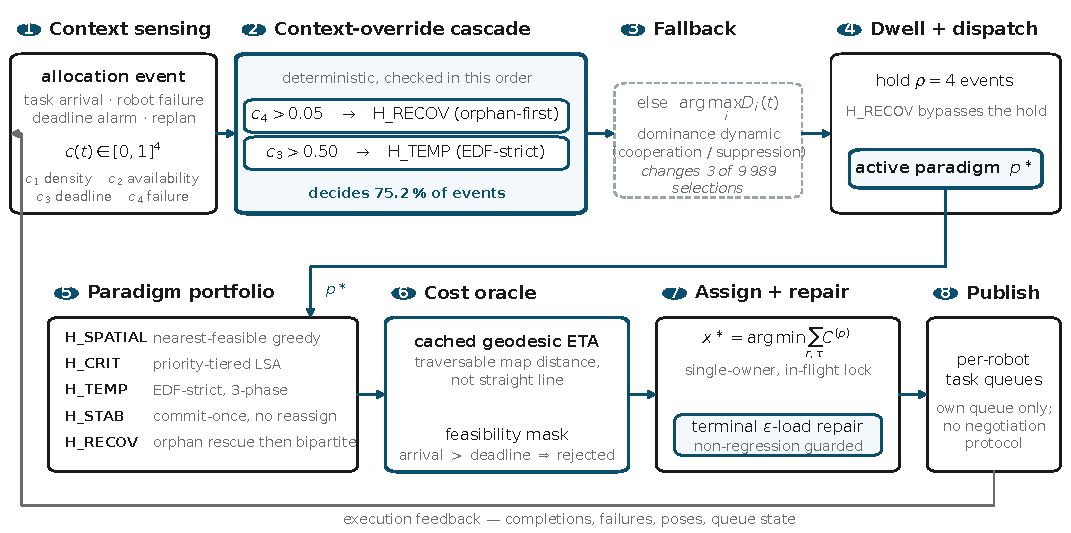
\includegraphics[width=\textwidth]{fig1.pdf}
  \caption{Tek bir tahsis olayındaki bilgi akışı. \textbf{Satır A} etkin
  politikayı belirler. Sistem durumu bağlam vektörüne dönüştürülür (1), arıza
  ve son teslim kuralları öncelik sırasıyla denetlenir (2), bu kurallar
  tetiklenmezse baskınlık puanları kullanılır (3) ve bekleme kuralından sonra
  etkin politika $p^\ast$ yayımlanır (4). \textbf{Satır B} seçilen politikayı robot kuyruklarına
  dönüştürür. Portföy görev sırasını belirler (5), geodezik seyahat kestirimi
  robot--görev çiftlerini maliyetlendirir ve uygun olmayan çiftleri eler (6),
  atama tek sahiplik ve yürütülen görev kilitleri altında yapılır (7), son yük
  dengeleme adımından sonra robot kuyrukları yayımlanır (8). Yürütme geri
  bildirimi yeni bağlam hesabına aktarılır. Sabit katsayılar
  Bölüm~\ref{sec:method-config}'de verilmiştir.}
  \label{fig:mechanism}
\end{figure}

\subsection{Algoritma ve Hesaplama Karmaşıklığı}
\label{sec:ahe-loop}

Algoritma~\ref{alg:ahe}, seçicinin bir atama çevrimindeki yürütme sırasını
gösterir. Yeni veya henüz atanmamış görevler, robot ya da navigasyon durumu
güncellemeleri ve periyodik denetim çevrimi tetikleyebilir. Çevrim sonunda yalnız
robot kuyrukları yayımlanır. $D_k$, $A$, $S$, $V$ ve tam maliyet matrisi
merkezi yönetici düğümünde tutulur.

\begin{algorithm}[t]
\caption{AHE-MRTA Olay Çevrimi}
\label{alg:ahe}
\begin{algorithmic}[1]
\REQUIRE $\mathcal R$, $\mathcal T(t_k)$, önceki kuyruklar, $D_k$,
         $p_{k-1}$, bekleme sayacı $h_k$ ve sabit $A,S,V,M$
\STATE $c_k\gets\textsc{BağlamVektörü}(\mathcal R,\mathcal T(t_k))$
\STATE Uygunluk maskesini, sahipsiz görev havuzunu ve yürütme kilitlerini güncelle
\STATE $\mathbf v_k\gets(\cos(V_i,c_k))_{i=1}^{5}$ ve
       $\mathbf p_k,\mathbf b_k\gets\textsc{GeriBeslemeVeArızaDesteği}()$
\STATE $D_{k+1}\gets\textsc{BaskınlıkGüncelle}(D_k,\mathbf v_k,
       \mathbf p_k,\mathbf b_k,A,S)$ \hfill \COMMENT{Denk.~\eqref{eq:dominance}}
\STATE $w_k\gets\textsc{AğırlıkÜret}(D_{k+1},c_k,M)$
       \hfill \COMMENT{Denk.~\eqref{eq:weights}}
\STATE $\tilde p_k\gets\textsc{HamSeçim}(c_k,D_{k+1})$
       \hfill \COMMENT{Denk.~\eqref{eq:dispatch}}
\STATE $(p_k,h_{k+1})\gets\textsc{BeklemeUygula}(\tilde p_k,p_{k-1},h_k)$
\STATE $x_k\gets\textsc{Politika}_{p_k}(\mathcal R,\mathcal T(t_k),w_k)$
       \hfill \COMMENT{Tablo~\ref{tab:hormones}}
\IF{son yük dengeleme evresindeyse}
  \STATE $x_k\gets\textsc{EpsilonYükDengele}(x_k,d_G,\epsilon)$
\ENDIF
\STATE $x_k\gets\textsc{TekSahipVeYürütmeKilidi}(x_k)$
\STATE Robot kuyruklarını yayınla ve $(D_{k+1},p_k,h_{k+1})$ durumunu sakla
\end{algorithmic}
\end{algorithm}

\label{sec:method-config}

Algoritmanın yapılandırması bütün senaryo ve filo ölçeklerinde sabittir:
$\alpha=0.65$, $\beta=0.40$, $\gamma=0.20$,
$\eta=\lambda=0.12$, $\delta=0.20$, $T_w=0.3$ ve $K_{\rm dwell}=4$.
Temel maliyet ve toparlanma profilleri sırasıyla
\[
w_0=(0.34,0.10,0.04,0.16,0.10,0.22,0.04)
\]
ve
\[
w_{\rm rec}=(0.55,0.04,0.03,0.22,0.09,0.05,0.02)
\]
olarak tanımlanır. Kanal sırası, Denklem~\eqref{eq:weight-map} öncesindeki
açıklamayla aynıdır. Bu değerler olay veya senaryo temelinde yeniden öğrenilmez
ya da ayarlanmaz.

Bağlam, baskınlık, geçersiz kılma ve bekleme güncellemeleri sabit boyutlu
olduğundan $O(1)$ karmaşıklığa sahiptir. Hesaplama yükünün baskın bölümü,
politika içindeki doğrusal toplam atama işlemidir. Tek bir kare atama geçişinin
en kötü durum karmaşıklığı
$O\!\left(\max(n,m_k)^3\right)$'tür. Geodezik sorguların
önbelleğe alınması yinelenen hedef sorgularını azaltır. Yük dengeleme ise sabit
sayıda yerel görev aktarımıyla sınırlandırılır. Bu nedenle toplam hesaplama
yükünü seçiciden çok, etkin politika ile isteğe bağlı rota ve yük dengeleme
bileşenleri belirler.

%==============================================================================
\section{Deneysel Yöntem}
\label{sec:setup}

\subsection{Araştırma Soruları ve Değerlendirme Düzeyleri}
\label{sec:planes}

Deneysel değerlendirme üç araştırma sorusuna göre düzenlenmiştir. AS1, tam
yöntemin robot
arızası ve son teslim baskısı altında tahsis kalitesini artırıp artırmadığını
inceler. AS2, gözlenen başarımın navigasyon belirsizliği ve kapalı çevrim
yürütme eklendiğinde korunup korunmadığını araştırır. AS3, etkinin politika
portföyü, çevrim içi seçici, seyahat kestirimi ve yük dengeleme bileşenleri
arasında nasıl dağıldığını inceler.

Bu soruları birbirinden ayırmak için üç değerlendirme düzeyi kullanılmıştır.
Navigasyondan bağımsız benzetim yalnızca tahsis kararlarını ve kuyruk sırasını
değerlendirir. Stokastik navigasyon modeli, hedefe ulaşamama ve yeniden deneme
durumlarını ekler. Kapalı çevrim Gazebo/ROS\,2 değerlendirmesi ise fiziksel
benzetimi ve Nav2 yürütmesini uçtan uca çalıştırır. Üç düzeyin sonuçları ayrı
raporlanır ve Tartışma bölümünde birlikte yorumlanır.

\subsection{Deney Platformu ve Test Koşulları}
\label{sec:hardware}
Tüm deneyler Intel Core i7-11800H iş istasyonunda çalıştırıldı. Makine
sekiz fiziksel çekirdeğe, 16 iş parçacığına, 2.30~GHz temel saate, 16~GiB
DDR4 belleğe, Ubuntu\,24.04~LTS işletim sistemine ve Linux\,6.17 çekirdeğine
sahiptir. Sistemde NVIDIA RTX\,3050\,Mobile grafik işlemcisi bulunmasına rağmen
tescilli sürücü kurulu değildir. Bu nedenle Gazebo ve RViz, Mesa llvmpipe
yazılımsal görüntülemesini kullanır
(\nolinkurl{LIBGL_ALWAYS_SOFTWARE=1}, \nolinkurl{GALLIUM_DRIVER=llvmpipe}).
Deneylerde grafik işlemci hızlandırması kullanılmamış ve hesaplama yükü
merkezi işlemci tarafından karşılanmıştır.

\textbf{Gazebo Harmonic} (gz-sim\,8.x)~\cite{koenig2004design},
\textbf{ROS\,2 Jazzy}~\cite{macenski2022ros2} ve \textbf{Nav2}
\cite{macenski2023nav2} kullanıldı. Robotlar \textbf{TurtleBot3 Waffle Pi}
modelidir \cite{robotis2023turtlebot3}. Her robotta 360-ışınlı iki boyutlu
lidar (5~Hz, 8~m menzil), 200~Hz IMU ve diferansiyel-tahrik denetleyicisi
vardır ($v_{\max}{=}0.26$~m/s, $\omega_{\max}{=}1.82$~rad/s).

Her robot, kendi ROS\,2 ad uzayında bağımsız bir Nav2 yaşam döngüsü çalıştırır.
Yazılım yığını, 0.40~m şişirme yarıçapına sahip küresel ve yerel maliyet
haritalarını, Regulated Pure Pursuit denetleyicisini ve davranış ağacı
gezginini içerir. Referans konum, her robotun başlangıç konumuna sabitlenen
statik \texttt{map}$\to$\texttt{odom} dönüşümüyle sağlanır. Bu deneysel tercih,
tahsis politikasının etkisini yerelleştirme hatasından ayırır
(Bölüm~\ref{sec:limitations}). \texttt{ros\_gz\_bridge}, her robot için
\texttt{/scan}, \texttt{/odom}, \texttt{/cmd\_vel}, \texttt{/joint\_states}
ve dönüşüm çerçevelerini aktarır. Ayrı bir aktarıcı, görüntüleme için robotların
ad uzaylarındaki dönüşüm ağaçlarını birleştirir. Bütün yöntemler aynı Nav2
parametrelerini kullanır. Şekil~\ref{fig:system}, merkezi yönetici ile her
robota ait Nav2 yaşam döngüsünün bağlantısını gösterir.

AHE-MRTA*, geodezik seyahat kestirimi ve son yük dengeleme etkin durumdayken
değerlendirilmiştir. Bu iki bileşen başlatma sırasında açıkça etkinleştirilir.
Tahsis edicinin yerleşik ayarları ise ablasyonda kullanılan Öklid mesafeli ve
yük dengelemesiz başvuru yapılandırmasını üretir. Dolayısıyla yürütülen sistemi
yöntem adından çok yapılandırma anahtarları belirler. Etkin anahtarlar hem her
koşunun üstverisine hem de kampanya dizinine kaydedilir. Böylece aynı yöntem
adını taşıyan farklı yapılandırmalar birbirinden ayrılır. Tahsis edici,
kampanya betikleri ve tablo ile şekilleri ham kayıtlardan üreten çözümleme
betikleri makaleyle birlikte sunulmaktadır.

Deney arenası, $20{\times}20$~m boyutlarında duvarlarla çevrili kapalı bir
ortamdır. Ortasında 1.5~m genişliğinde bir geçit bulunan iki yatay duvar, üst
ve alt koridorları oluşturur. Yan duvarlarda iki sıra kare sütun
($0.5{\times}0.5$~m), koridorlarda ise dört silindirik engel ($r{=}0.35$~m)
bulunur. Engellerin dışında ve birbirinden en az 1~m uzakta 42 sabit denetim
noktası tanımlanmıştır. Her koşudaki görev kümesi, bu noktalardan ilgili
rastgelelik tohumu kullanılarak belirlenimci biçimde örneklenir.
Şekil~\ref{fig:scenario-maps} arena düzenini, robotların başlangıç konumlarını
ve örnek görev kümelerini gösterir.

\begin{figure}[t]
  \centering
  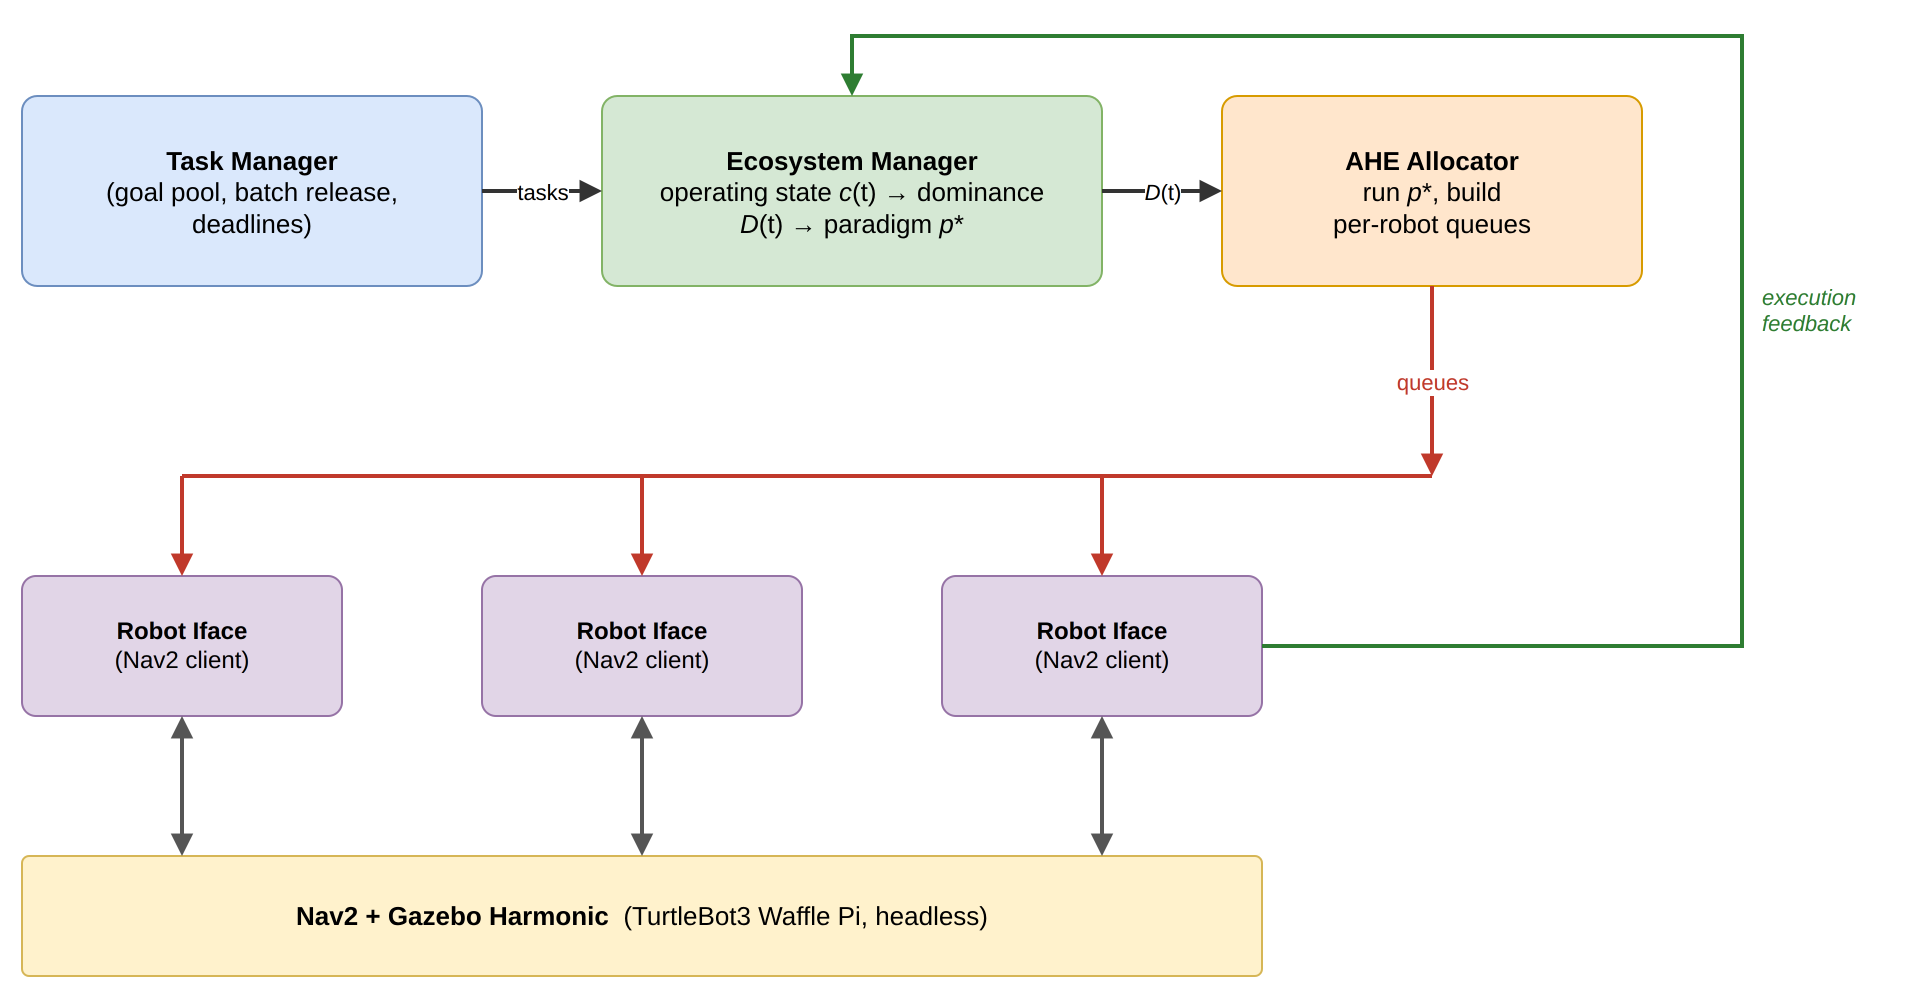
\includegraphics[width=0.85\textwidth]{fig2.drawio.png}
  \caption{Sistem mimarisi. Merkezi yönetici seçici durumunu günceller,
  etkin politikayı belirler ve ROS\,2 konuları üzerinden her robot için görev
  kuyruğu yayımlar. Her robot kendi Nav2 yaşam döngüsünü çalıştırır ve
  tamamlama, arıza ve gecikme geri bildirimini yöneticiye gönderir.}
  \label{fig:system}
\end{figure}

\begin{figure}[t]
  \centering
  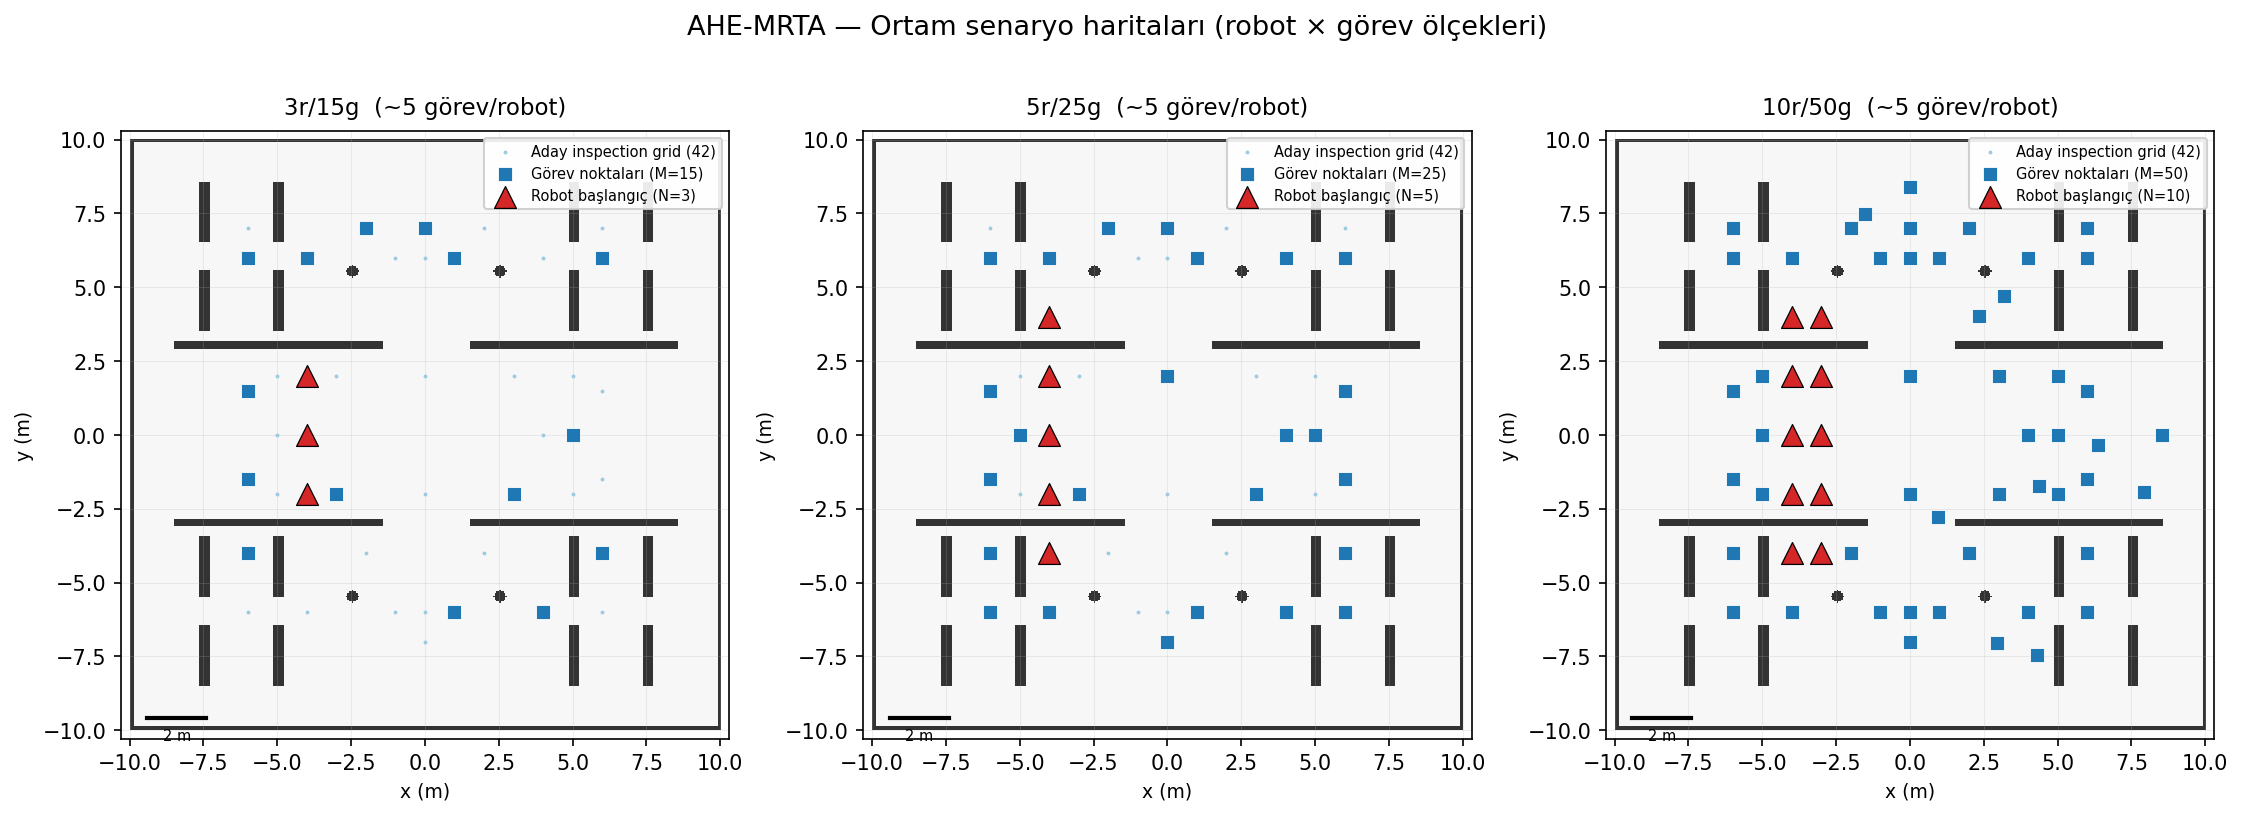
\includegraphics[width=0.85\textwidth]{scenario_maps_panel.png}
  \caption{Filo ölçeğine göre arena düzenleri. \textbf{Sol:}
  3 robot ve 15 görev için robotlar tek merkez sütunundadır. \textbf{Orta:}
  5 robot ve 25 görev için iki başlangıç sütunu vardır. \textbf{Sağ:} 10 robot
  ve 50 görev için beş sütunun tamamı kullanılır.
  Mavi yıldızlar tohum\,1 için görev hedeflerini, renkli üçgenler robot
  başlangıç konumlarını gösterir. Tüm ara noktalar engelsizdir.}
  \label{fig:scenario-maps}
\end{figure}

\label{sec:scales}
Üç Gazebo filo ölçeği değerlendirilmiştir (Tablo~\ref{tab:scales}). Her
ölçek--yoğunluk hücresinde 60 koşu vardır ($4$ yöntem $\times$ $3$ senaryo
$\times$ $5$ tohum). Birincil 5 robotlu hücrede ise yöntem ve senaryo başına
20 tohum kullanılmış ve toplam 240 koşu yürütülmüştür.

\begin{table}[h]
\centering
\caption{Kapalı çevrim Gazebo değerlendirmesinde kullanılan filo ölçekleri.}
\label{tab:scales}
\renewcommand{\arraystretch}{1.15}
\begin{tabular}{@{}ccccc@{}}
\toprule
Ölçek & Robot & Görev & Yoğunluk & Toplam deney \\
\midrule
3r-az    & 3 & 9  & 3.0 g/r & 60 \\
3r-orta  & 3 & 15 & 5.0 g/r & 60 \\
3r-yüksek& 3 & 24 & 8.0 g/r & 60 \\
5r-orta  & 5 & 25 & 5.0 g/r & 240 \\
10r-orta & 10 & 50 & 5.0 g/r & 60 \\
\midrule
\multicolumn{4}{l}{\textbf{Toplam Gazebo deneyi}} & \textbf{480} \\
\bottomrule
\end{tabular}
\end{table}


$N{>}3$ olduğunda bazı robotların
\texttt{odom}$\!\rightarrow\!$\texttt{base\_link} dönüşümü, maliyet haritası
etkinleştirildikten sonra hazır olmuştur. Bu başlatma sırası sorununu gidermek
için $i$. robotun etkinleştirilmesi 3 ve 5 robotlu koşullarda $6i$~s, 10
robotlu koşulda ise $20i$~s geciktirilmiştir. Ayrıca düğüm başlatılırken birim
dönüşüm yayımlanmıştır. Bütün ölçeklerde aynı arena, engel haritası ve Nav2
parametreleri kullanılmıştır.

\label{sec:scenarios}
Üç senaryo, farklı tahsis gereksinimlerini değerlendirmek üzere
tanımlanmıştır.

Her koşunun süresi $T_{\max}=900$~s ile sınırlandırılmıştır. Bu sürenin sonunda
açık kalan görevler tamamlanmamış sayılır (Bölüm~\ref{sec:metrics}). Her görev
için bağımsız olarak $\pi_\tau\sim\mathcal U\{1,2,3\}$ önceliği,
$\mathcal U[2,8]$~s hizmet süresi ve $d_\tau=t_0+\Delta_\tau$ son teslim
zamanı üretilir. Senaryolar, $\Delta_\tau$ zaman bütçesi, görevlerin geliş
takvimi ve robot arızasının varlığı bakımından farklılaşır.

\begin{itemize}
  \item \textbf{Robot arızası (\texttt{robot\_failure}):} Bütün görevler
        $t_0$ anında etkinleştirilir ve
        $\Delta_\tau\sim\mathcal U[90,300]$~s kullanılır. Önceden belirlenen
        bir robot, her tohum için düzgün dağılımdan seçilen sapmayla
        $t=45\pm5$~s'de devre dışı bırakılır. Bu zaman aralığı, robotun görev
        üstlenmiş olmasını sağlayacak kadar geç seçilmiştir. Robotun
        tamamlanmamış görevleri sahipsiz kalır ve yeniden atanır. Senaryo,
        arıza sonrası toparlanmayı değerlendirir.

  \item \textbf{Birleşik stres (\texttt{mixed\_stress}):} Aynı arıza olayı,
        kademeli görev gelişi ve daha dar bir zaman bütçesiyle birleştirilir.
        Görevler $t=0$, $30$ ve $60$~s'de üç dalga
        hâlinde gelir ($\lfloor M/3\rfloor$, $\lfloor M/3\rfloor$ ve kalan)
        ve bütçe yarıya iner ($\Delta_\tau\sim\mathcal U[45,150]$~s).
        Son teslim zamanları $t_0$ anından itibaren hesaplandığı için sonraki
        dalgalardaki görevlerin kullanılabilir süresi daha kısadır. Tahsis
        edici, görev gelişlerini, öncelikleri ve robot arızasını birlikte ele
        almalıdır.

  \item \textbf{Son teslim baskısı (\texttt{deadline\_pressure}):} Robot
        arızası yoktur ve bütün görevler $t_0$ anında etkinleştirilir. Son
        teslim bütçesi nominal değerin $\%40$'ına indirilir
        ($\Delta_\tau\sim\mathcal U[36,120]$~s). Bu aralığın alt ucu,
        $v_{\max}$'da en uzak ara noktaya Nav2 seyahat süresinin altındadır.
        Dolayısıyla bazı görevlerin zamanında tamamlanması fiziksel olarak
        mümkün değildir. Bu senaryo, aciliyet temelli tahsis ile en erken son
        teslim zamanı önce (EDF) sıralamasını diğer politikalardan ayırır.
\end{itemize}

Arıza, rastgele seçilen bir robot yerine sabit bir robot indeksine uygulanır.
Bu sayede aynı tohum için toparlanma yükü bütün yöntemlerde aynıdır. Görev
konumları, öncelikler, hizmet süreleri, son teslim zamanları ve arıza anı
rastgelelik tohumu ile belirlenir ve dört yöntemin tamamında ortak tutulur.

\subsection{Karşılaştırma ve Ablasyon Yapılandırmaları}
\label{sec:baselines}
AHE-MRTA, portföyünde yer alan çevrim içi MRTA ailelerini temsil eden üç yöntem
uyarlamasıyla karşılaştırılmıştır. Bütün yöntemler aynı olay döngüsünü, ROS\,2
konu arayüzünü, Nav2 istemcisini ve varış süresi, aciliyet, öncelik ile yükten
oluşan maliyet girdilerini kullanır. Yöntemler yalnızca tahsis politikası
bakımından farklıdır. Denklem~\eqref{eq:queue-cap}'deki robot başına kuyruk
sınırı $Q$, ortak bir sabit değil, her politikanın yapılandırma öğesidir.
BiG-MRTA ve Consensus-DBTA için $Q{=}5$ kullanılır. RoSTAM-EA'da olay içindeki
kuyruk uzunluğu sınırlandırılmaz. AHE-MRTA'da ise arıza sonrası yeniden atamayı
kolaylaştırmak için $Q{=}2$ alınır ve son yük dengeleme aşamasında bu değer bir
artırılır. Kaynak çalışmada verilen parametreler korunmuş, belirtilmeyen
seçimler bu kıyaslama için sabitlenmiş ve raporlanmıştır. Dolayısıyla yöntem
adları, kaynak sistemlerin bağımsız ve eksiksiz yeniden uygulamalarını değil,
bu çalışmada kullanılan uyarlamaları ifade eder.

BiG-MRTA uyarlaması~\cite{ghassemi2022bigmrta}, sabit çok ölçütlü kenar
faydalarına sahip iki parçalı bir robot--görev grafiği kurar ve her olayda en
büyük ağırlıklı eşlemeyi çözer. Bir kez yapılan atama daha sonra yeniden ele
alınmaz. Bu yöntem, belirlenimci ve düşük karar gecikmeli sabit politika
karşılaştırmasını temsil eder. Yeniden planlamayı önler, ancak görev atanan
robot arızalandığında veya zaman bütçesi tükendiğinde görevi geri kazanmaz.

RoSTAM-EA uyarlaması~\cite{rostam2024selfadaptive}, aday atama vektörlerini her
tahsis olayında turnuva seçimi, çaprazlama ve mutasyon yoluyla geliştirir ve en
iyi bireyi uygular. Yöntem, öz-uyarlanır stokastik arama ailesini temsil eder.
Tek geçişli eşlemeye göre daha geniş bir atama uzayını araştırır, ancak karar
gecikmesi iki ile üç büyüklük mertebesi daha yüksektir. Ayrıca yeniden
eniyileme işlemi bağlam değişiminin nedenini açık biçimde temsil etmez.

Consensus-DBTA uyarlamasında~\cite{mahato2023consensus} her robot, en yüksek
değere sahip iki görev için teklifini paylaşır. Benzetilen ağ genelindeki
uzlaşma, her görevin kazananını belirler. Öncelik turları ise aynı robotun
birbiriyle çelişen görevleri kazanmasını önler. Bu yapı atamaları büyük ölçüde
kararlı tutar ve arıza sonrası görevlerin yeniden gönderilmesini sağlar.
Dağıtık açık artırma ve uzlaşma ailesini temsil eden yöntem, bu çalışmada temel
yöntemler arasındaki en yüksek tamamlama oranını vermiştir. Bununla birlikte
yinelenen teklif turları, arızalara veya son teslim baskısındaki hızlı artışlara
verilen tepkiyi geciktirebilir.

Bu üç yöntem, AHE-MRTA'dan yalnızca politika seçimi bakımından değil, tahsis
mantığı bakımından da ayrılır. Bu nedenle dış yöntemlerle yapılan karşılaştırma,
seçicinin bağımsız etkisini belirleyen bir ablasyon değildir. Bu etki, biri
stokastik navigasyon modelinde (Bölüm~\ref{sec:ablation}), diğeri önceden
belirlenmiş ve eşleşmiş kapalı çevrim deneyinde
(Bölüm~\ref{sec:gazebo-ablation}) olmak üzere iki ayrı ablasyonla incelenmiştir.

Karşılaştırılan yöntemler aynı olay döngüsünü, arayüzleri ve maliyet girdilerini
paylaşsa da kaynak sistemlerin eksiksiz yeniden üretimleri değildir. Bu nedenle
dört yöntemli karşılaştırma, ortak yürütme yığınındaki uyarlamaları değerlendirir
ve atıf verilen algoritmalar için genel bir üstünlük sıralaması oluşturmaz.
Seçicinin kapalı çevrim etkisini ayırmak amacıyla sabit politikaları içeren
kontrollü Gazebo ablasyonu kullanılmıştır. Bu deneyin desteklediği çıkarımların
sınırı Bölüm~\ref{sec:gazebo-ablation}'da açıklanmaktadır.

Stokastik navigasyon modeli üzerindeki ablasyonda seçici, portföydeki her sabit
politika ile ayrı ayrı değiştirilmiştir. Bağlam geçersiz kılmaları ve
toparlanma desteği de diğer bileşenler sabit tutularak ayrı ayrı devre dışı
bırakılmıştır. Eşleşmiş kapalı çevrim ablasyonu, tam yöntemi geçersiz kılma
kuralı olmayan yapılandırma, sabit EDF politikası ve sabit sahipsiz görev önce
politikasıyla aynı tohumlar üzerinde karşılaştırmıştır. Sabit uzamsal açgözlü
yapılandırma, önceden belirlenen dört yapılandırmaya sonradan eklenen keşifsel
bir karşılaştırma olarak ayrı değerlendirilmiştir.

\subsection{Değerlendirme Ölçütleri ve İstatistiksel Analiz}
\label{sec:metrics}

Tamamlanan görevler $\mathcal T^{\rm done}$ ve istenen bütün görevler
$\mathcal T^{\rm req}$ kullanılarak birincil sonuçlar
\begin{equation}
  \max\ \mathrm{CR}=
  \frac{|\mathcal{T}^{\rm done}|}{|\mathcal{T}^{\rm req}|},
  \qquad
  \min\ \mathrm{DVR}=
  \frac{|\{\tau:d_\tau<\infty\ \wedge
  (t_\tau^{\rm c}>d_\tau\ \vee\ \tau\notin\mathcal{T}^{\rm done})\}|}
  {\max\!\bigl(1,|\{\tau:d_\tau<\infty\}|\bigr)}
  \label{eq:primary-outcomes}
\end{equation}
biçiminde tanımlanır. Ayrıca toplam tamamlanma süresi, bütün görevlerdeki
ortalama gecikme, arıza sonrası toparlanma süresi, iş yükü dengesi (Jain), görev
yeniden gönderim oranı, yürütme kesintileri, karar gecikmesi ve mesaj sayısı
raporlanır. Gerektiğinde toplam seyahat mesafesi de verilir. CR ve DVR
birincil sonuç ölçütleridir. Diğer ölçütler verimliliği ve ödünleşimleri
gösterir. Tahsis olayı başına karar süresi hedefi 50~ms'dir.

Gecikme yalnızca tamamlanan görevler üzerinden hesaplandığında, tamamlanmadan
bırakılan zor görevler değerlendirme dışında kalır. Bu sağkalım yanlılığını
önlemek için gecikme ve DVR, istenen görevlerin \emph{tamamı} üzerinden
hesaplanmıştır.
$\mathcal{T}$ istenen görev kümesi, $t^{\mathrm{a}}_\tau$ etkinleşme zamanı,
$t^{\mathrm{c}}_\tau$ tamamlama zamanı ve $T_{\max}$ çalışma ufku olsun.
Bitmeyen görevin gecikmesi ufukta sağdan sansürlenir:
\begin{equation}
  \delta_\tau =
  \begin{cases}
    t^{\mathrm{c}}_\tau - t^{\mathrm{a}}_\tau, & \tau \text{ tamamlandı},\\[2pt]
    T_{\max} - t^{\mathrm{a}}_\tau,             & \tau \text{ bitmedi},
  \end{cases}
  \qquad
  \overline{\delta} = \frac{1}{|\mathcal{T}|}\sum_{\tau\in\mathcal{T}}\delta_\tau ,
  \label{eq:fairdelay}
\end{equation}
Son teslim zamanı bulunan bir görev geç tamamlandığında veya hiç
tamamlanmadığında Denklem~\eqref{eq:primary-outcomes} uyarınca ihlal sayılır.
Bu kural bütün yöntemlere ve filo ölçeklerine aynı biçimde uygulanır. Ek olarak,
yalnızca tamamlanan görevleri kullanan geleneksel gecikme ve DVR değerleri de
kaydedilmiştir. CR${=}1$ olduğunda iki hesaplama aynı sonucu verir. Yöntem bazı
görevleri tamamlamadığında sonuçlar birbirinden ayrılır.

İstatistiksel analizde her senaryo için Bonferroni düzeltmeli, ikili ve iki
yönlü Mann--Whitney U testleri kullanılmıştır. Üç temel yöntem ve yedi ölçüt
için senaryo başına 21 test yapılmıştır. Birincil 5 robotlu ölçekte her hücre
$n{=}20$ koşu içerir ve tek yoğunlukta 25 görev kullanılır. Üç robotlu ölçekte
üç yoğunluk birleştirilerek $n{=}15$ elde edilmiştir. On robotlu ölçekte ise
$n{=}5$ koşu vardır. Özellikle küçük örneklemli hücrelerde farkın büyüklüğünü
göstermek için Cliff $\delta$ etki büyüklüğü de raporlanmıştır. On robotlu
Gazebo hücreleri $n{=}5$ olduğu için yalnızca betimleyici olarak
yorumlanmıştır. İstatistiksel olarak anlamlı olmayan veya çoklu karşılaştırma
düzeltmesini geçmeyen sonuçlardan yöntem üstünlüğü çıkarılmamıştır.
Navigasyondan bağımsız değerlendirmede hücre başına 100, birincil stokastik
navigasyon değerlendirmesinde ise 500 tohum kullanılmıştır. Bu iki kampanya
ayrı kontrollü deneylerdir. Gazebo sonuçları genel konuşlandırma başarımını
değil, değerlendirilen fizik ve navigasyon yığınındaki davranışı gösterir.

%==============================================================================
\section{Bulgular}
\label{sec:results}

\subsection{Navigasyondan Bağımsız Değerlendirme}
\label{sec:results-sim}

Navigasyondan bağımsız ortamda (Böl.~\ref{sec:planes}) tahsis edici ve yürütme
modeli, aynı şişirilmiş doluluk haritası üzerinde geodezik mesafeyi kullanır.
Bu deney, yerel planlayıcıdan kaynaklanan değişkenliği dışlayarak tahsis
kararlarını, kuyruk sıralamasını ve arıza sonrası toparlanmayı değerlendirir.

\begin{table}[t]
\centering
\caption{AHE-MRTA navigasyon-ba\u{g}\i ms\i z allocation-only sonu\c{c}lar\i (h\"ucre ba\c{s}\i na 100 tohum). Navigasyon belirlenimci olarak ba\c{s}ar\i l\i d\i r; mesafe, payla\c{s}\i lan \c{s}i\c{s}irilmi\c{s} doluluk haritas\i \"uzerindeki geodezik yol uzunlu\u{g}udur.}
\label{tab:allocation}
\small
\setlength{\tabcolsep}{3.5pt}
\resizebox{\textwidth}{!}{%
\begin{tabular}{llrrrrrrrr}
\toprule
\textbf{\"Ol\c{c}ek} & \textbf{Senaryo} & \textbf{Uyg.} & \textbf{CR} & \textbf{DVR} & \textbf{Jain$_{aktif}$} & \textbf{Jain$_{mesafe}$} & \textbf{Gecikme (s)} & \textbf{Mesafe} & \textbf{Karar (ms)} \\
\midrule
3r/15t & Robot arızası & 0.968 & 1.000 & 0.036 & 0.994 & 0.841 & 84.3 & 148.6 & 0.066 \\
3r/15t & Karışık stres & 0.647 & 1.000 & 0.353 & 0.992 & 0.828 & 55.5 & 142.7 & 0.068 \\
3r/15t & Deadline baskısı & 0.774 & 1.000 & 0.232 & 0.986 & 0.965 & 62.3 & 119.3 & 0.070 \\
\midrule
5r/25t & Robot arızası & 0.994 & 1.000 & 0.005 & 0.988 & 0.900 & 71.5 & 222.4 & 0.082 \\
5r/25t & Karışık stres & 0.727 & 1.000 & 0.271 & 0.983 & 0.886 & 40.7 & 201.6 & 0.088 \\
5r/25t & Deadline baskısı & 0.835 & 1.000 & 0.164 & 0.985 & 0.960 & 57.0 & 172.8 & 0.090 \\
\midrule
10r/50t & Robot arızası & 1.000 & 1.000 & 0.000 & 0.988 & 0.923 & 64.8 & 408.4 & 0.140 \\
10r/50t & Karışık stres & 0.782 & 1.000 & 0.215 & 0.986 & 0.905 & 31.7 & 333.1 & 0.215 \\
10r/50t & Deadline baskısı & 0.888 & 1.000 & 0.116 & 0.987 & 0.945 & 53.5 & 303.6 & 0.169 \\
\bottomrule
\end{tabular}}
\end{table}


Tablo~\ref{tab:allocation}, AHE-MRTA sonuçlarını üç filo ölçeğinde ve hücre
başına 100 tohumla raporlar. Dokuz ölçek--senaryo hücresinin tamamında
CR${=}1.000$'dır. Buna karşılık, son teslim süresinden sonra tamamlanan görevler
puan almadığı için öncelik ağırlıklı zamanında tamamlama $0.647$ ile $1.000$
arasında değişir. Son teslim ihlal oranı robot arızasında $0.000$--$0.036$,
son teslim baskısında $0.116$--$0.232$ ve karışık streste $0.215$--$0.353$
aralığındadır. Aktif robotlar için Jain indeksi bütün ölçeklerde
$0.983$--$0.994$ arasında kalır. En yüksek karar gecikmesi, 10r/50g karışık
stres hücresinde ölçülen $0.215$~ms'dir.

Sahiplik denetimi sırasında, altı 10-robot tohumunda aynı görevin iki robot
tarafından eş zamanlı yürütülebildiği ve CR'nin 1.02'ye çıktığı belirlenmiştir.
Uçuş sırasındaki görevlere sahiplik kilidi uygulanmasının ardından bu tohumlar
ve 10-robot kampanyasının tamamı yeniden yürütülmüştür. Raporlanan sonuçlarda
bütün hücreler için CR tam olarak 1.000'dır.

Uygunluk, 3 robottan 10 robota geçildiğinde son teslim baskısında
$0.774\to0.888$, karışık streste ise $0.647\to0.782$ düzeyinde artar. Bu artış,
görev başına zaman bütçesi sabitken robot sayısının yükselmesinden kaynaklanır.
Navigasyondan bağımsız deney aynı zamanda politikaları birbirinden ayırır.
Birincil ölçekte AHE-MRTA'nın robot arızası, karışık stres ve son teslim
baskısındaki değerleri sırasıyla $0.994$, $0.727$ ve $0.840$'tır. En güçlü
temel yöntem olan BiG-MRTA'nın karşılık gelen değerleri $0.980$, $0.668$ ve
$0.733$'tür (Tablo~\ref{tab:fitness}, sol). Böylece yöntemler arasındaki fark,
navigasyon arızasından bağımsız olarak tahsis ve kuyruk sıralaması üzerinden
gözlenmektedir.

\subsection{Stokastik Navigasyon Vekili ve Ölçeklenebilirlik}
\label{sec:scalability}

Stokastik navigasyon vekilinde seyahat maliyeti, robot--görev grafiğinde sabit
süreli bir kenarla temsil edilir. Navigasyon sonucu ise konuma bağlı ve
stokastiktir. Başarısız olan bir hedef yeniden denenebilir. Bu nedenle
uygunluk, son teslim süresinden önce tamamlanan görevlerin öncelik ağırlıklı
oranının yanı sıra navigasyon arızasından sonra toparlanma başarımını da
içerir. Senaryo başına 500 tohum kullanıldığında AHE-MRTA, her iki deney
düzeyinde ve üç senaryonun tamamında en yüksek ortalamaya ulaşır
(Tablo~\ref{tab:fitness}). Temel yöntemlerle yapılan dokuz eşli
karşılaştırmanın sekizi anlamlıdır ve bu karşılaştırmalarda $p$ değerleri
$10^{-9}$ ile $10^{-76}$ arasındadır. Tek istisna, robot arızası altında
BiG-MRTA ile karşılaştırmadır ($+0.004$, $p{=}0.14$).

% GENERATED by scripts/make_proxy_tables.py -- do not edit by hand.
\begin{table}[t]
\centering
\caption{Tahsis uygunluğu (öncelik-ağırlıklı zamanında tamamlama), 500 tohum, 5 robot / 25 görev. \textbf{Sol:} mükemmel-navigasyon düzlemi, tahsis kalitesini yalıtır. \textbf{Sağ:} stokastik navigasyon vekili; burada Nav2 hedef arızası da bir göreve mal olabilir. AHE-MRTA her iki düzlemde ve her senaryoda öndedir; temel yöntemlere karşı eşli Wilcoxon karşılaştırmalarının biri dışında hepsi anlamlıdır (arıza senaryosunda AHE--BiG beraberedir). \textbf{Kalın} sütun en iyisidir.}
\label{tab:fitness}
\small
\setlength{\tabcolsep}{4pt}
\begin{tabular}{l ccc ccc}
\toprule
& \multicolumn{3}{c}{\textbf{Mükemmel nav (tahsis kalitesi)}} & \multicolumn{3}{c}{\textbf{Stokastik nav (dayanıklılık)}} \\
\cmidrule(lr){2-4}\cmidrule(lr){5-7}
\textbf{Yöntem} & RF & MS & DP & RF & MS & DP \\
\midrule
\textbf{AHE-MRTA*} & \textbf{0.994} & \textbf{0.727} & \textbf{0.840} & \textbf{0.384} & \textbf{0.263} & \textbf{0.349} \\
BiG-MRTA & 0.980 & 0.668 & 0.733 & 0.380 & 0.229 & 0.284 \\
RoSTAM-EA & 0.935 & 0.643 & 0.679 & 0.333 & 0.225 & 0.227 \\
Cons-DBTA & 0.978 & 0.642 & 0.729 & 0.364 & 0.217 & 0.258 \\
\bottomrule
\end{tabular}
\end{table}


Birincil ölçekte hiçbir yöntem üst sınıra ulaşmaz (25 görev ve 5 robot,
Tablo~\ref{tab:fitness}, sol). Navigasyon arızası bulunmadığında AHE-MRTA'nın
robot arızası, karışık stres ve son teslim baskısındaki değerleri sırasıyla
$0.994$, $0.727$ ve $0.840$'tır. En güçlü temel yöntemin değerleri $0.980$,
$0.668$ ve $0.733$'tür. Stokastik navigasyonda yöntemlerin değerleri düşmekle
birlikte sıralama korunur (Tablo~\ref{tab:fitness}, sağ). AHE-MRTA için
$0.384$, $0.263$ ve $0.349$ olan değerler, en güçlü temel yöntemde $0.380$,
$0.229$ ve $0.284$'tür. Robot arızasında BiG-MRTA ile fark anlamlı değildir.
En büyük fark son teslim baskısı altında gözlenir.

Yapılandırma tutarlılığı denetiminde, simülatörün önceki sürümündeki senaryo
parametrelerinin tanımlanan değerlerden saptığı belirlenmiştir
(Bölüm~\ref{sec:scenarios}). Son teslim baskısı için öngörülen
$\mathcal U[36,120]$~s yerine
$\mathcal U[200,400]$~s kullanılmış, karışık stres için yarıya indirilmiş zaman
bütçesi ve kademeli görev gelişleri uygulanmamıştır. Bu yapılandırma, yöntemler
arasındaki ayrımı azaltmıştır. Raporlanan deneylerde iki düzey de senaryo
tanımlarını Gazebo yürütücüsüyle ortak modülden okumaktadır. Otomatik tutarlılık
testi, iki tanım ayrıştığında başarısız olacak biçimde yapılandırılmıştır.
Stokastik vekil tıkanıklığı, yeniden planlama gecikmesini ve kapalı çevrim
toparlanma süresini modellemez. Bu nedenle kapalı çevrim sonuçlarının yerine
geçmez ve seçici mekanizmanın katkısını tek başına belirlemez. İlgili Gazebo
sonuçları Bölüm~\ref{sec:results-gazebo}'da, eşleşmiş mekanizma karşılaştırması
ise Bölüm~\ref{sec:gazebo-ablation}'da sunulmaktadır. Vekil sonuçları
Şekil~\ref{fig:fitness}'te özetlenmiştir.

\begin{figure}[t]
  \centering
  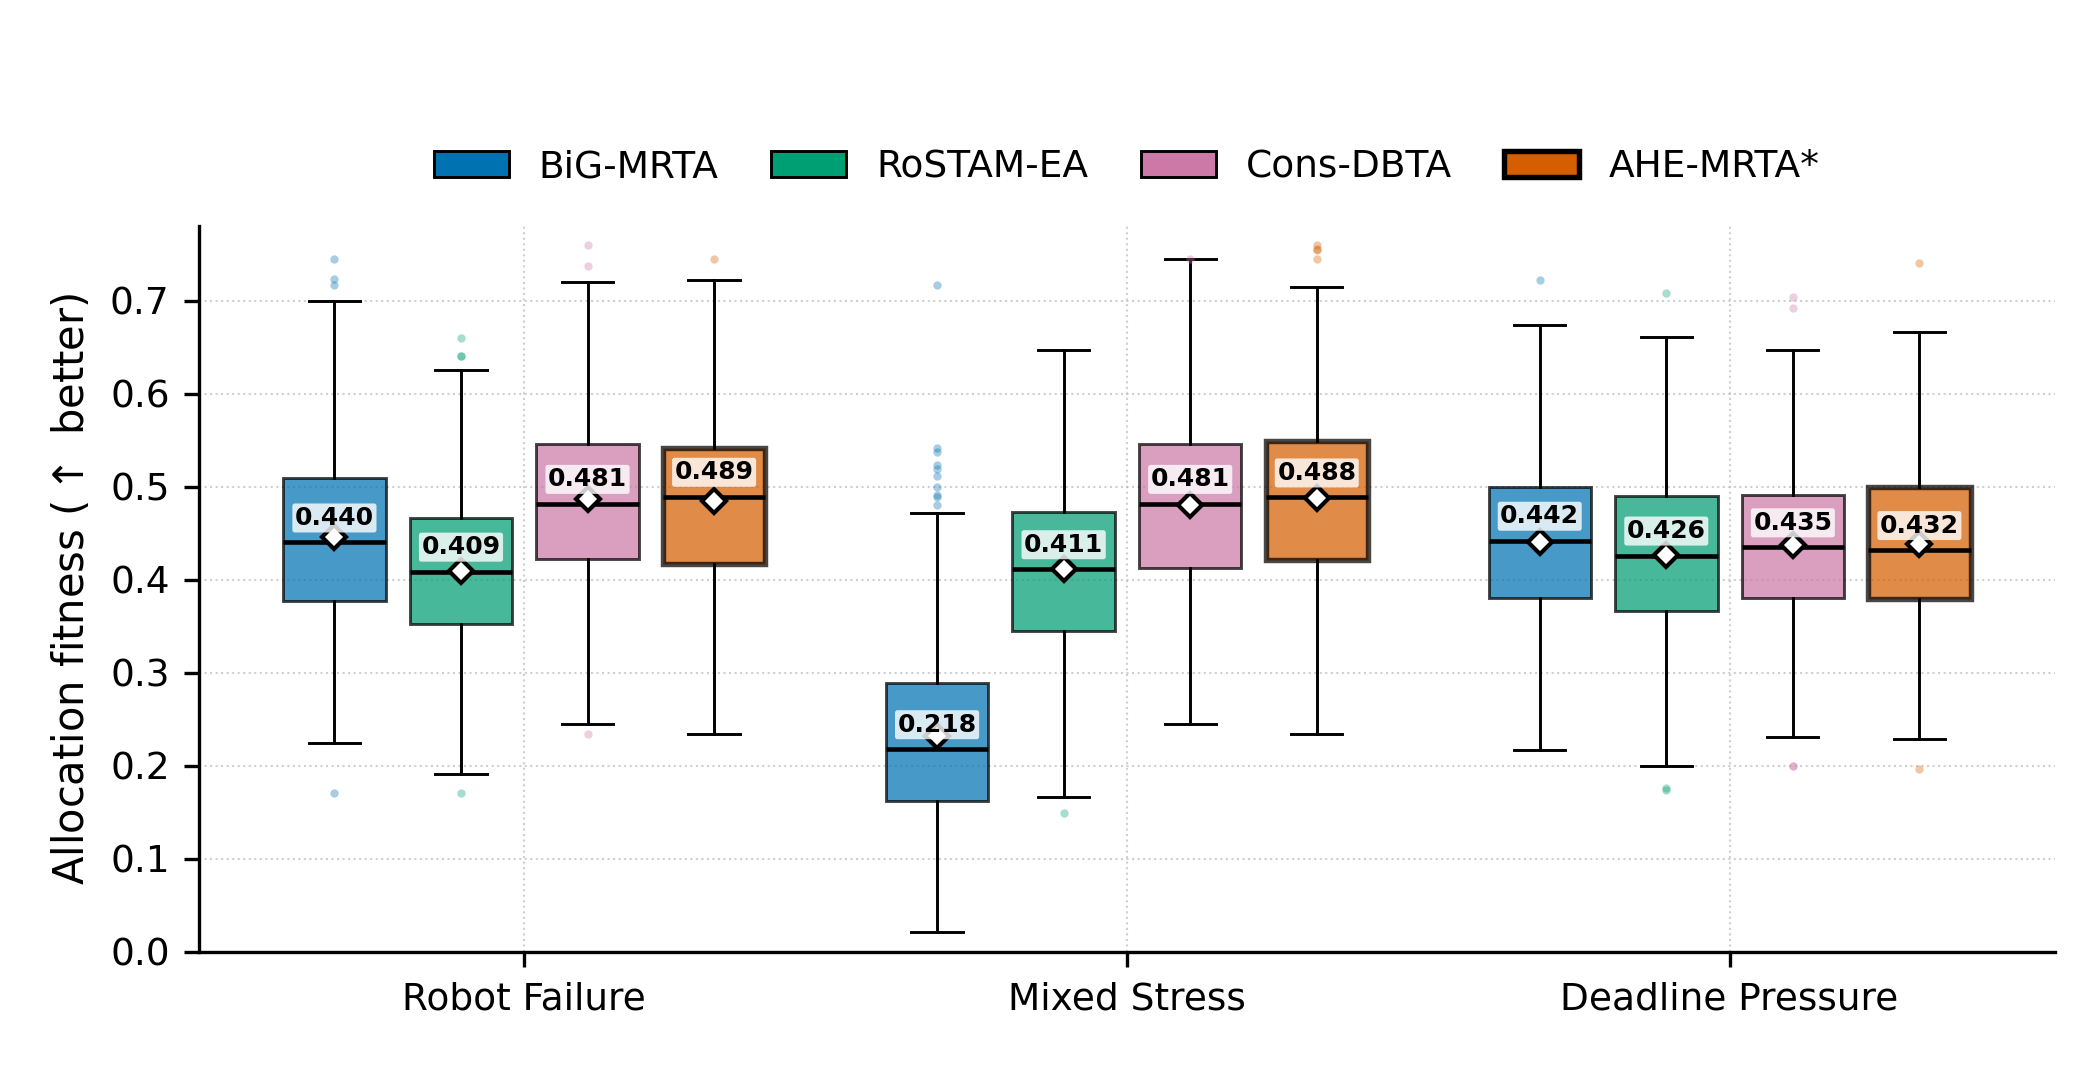
\includegraphics[width=0.80\textwidth]{fitness_comparison.png}
  \caption{Birincil 5-robot/25-görev ölçeğinde stokastik navigasyon vekili
  uygunluğu (hücre başına 500 tohum). Kutular çeyrekler arası aralığı, orta
  çizgiler medyanı (değeri her kutunun üzerinde yazılıdır), eşkenar dörtgenler
  ortalamayı, bıyıklar $1{,}5$ çeyrekler arası aralığı ve noktalar aykırı
  değerleri gösterir. AHE-MRTA her senaryoda öndedir. Her temel yönteme karşı
  yapılan eşli Wilcoxon karşılaştırmalarının dokuzdan sekizi anlamlıdır,
  istisna robot arızasında BiG-MRTA ile eşitliktir ($p{=}0.14$).}
  \label{fig:fitness}
\end{figure}

Vekil düzeyindeki ölçeklenebilirlik deneyinde dört yöntem
$N\in\{3,5,10\}$ robotla, robot başına beş görev ($M=5N$), hücre başına 100
tohum ve üç senaryo kullanılarak değerlendirilmiştir. Toplam 3.600 koşu
gerçekleştirilmiştir. Kapalı çevrim Gazebo deneyleri de 3, 5 ve 10 robot
ölçeklerini kapsamaktadır. Tablo~\ref{tab:scalability} ve
Şekil~\ref{fig:scalability}, vekil sonuçlarının senaryolar üzerindeki
ortalamalarını göstermektedir.

% GENERATED by scripts/make_proxy_tables.py -- do not edit by hand.
\begin{table}[t]
\centering
\caption{Ölçeklenebilirlik (stokastik navigasyon vekili, geodezik yürütme
modeli, 100 tohum ve sabit yoğunluk 5 görev/robot). Değerler senaryoların
ortalamasıdır. Uygunluk $\uparrow$, gecikme (ms) $\downarrow$. Her ölçekte en
iyi değer \textbf{kalın} gösterilmiştir. Kapalı çevrim Gazebo deneyleri 3, 5 ve
10 robotlu filoları kapsamaktadır.}
\label{tab:scalability}
\small
\setlength{\tabcolsep}{4pt}
\begin{tabular}{l cc cc cc }
\toprule
& \multicolumn{2}{c}{\textbf{3 robot}} & \multicolumn{2}{c}{\textbf{5 robot}} & \multicolumn{2}{c}{\textbf{10 robot}} \\
\cmidrule(lr){2-3}\cmidrule(lr){4-5}\cmidrule(lr){6-7}
\textbf{Yöntem} & Uyg. & Gec. & Uyg. & Gec. & Uyg. & Gec. \\
\midrule
\textbf{AHE-MRTA*} & \textbf{0.300} & 0.12 & \textbf{0.329} & 0.20 & \textbf{0.326} & 0.54 \\
BiG-MRTA & 0.267 & 0.02 & 0.293 & 0.05 & 0.298 & 0.17 \\
RoSTAM-EA & 0.249 & 1.93 & 0.261 & 3.48 & 0.245 & 7.00 \\
Cons-DBTA & 0.257 & \textbf{0.02} & 0.276 & \textbf{0.03} & 0.290 & \textbf{0.05} \\
\bottomrule
\end{tabular}
\end{table}


AHE-MRTA, her filo ölçeğinde en yüksek vekil uygunluğunu elde eder
(Tablo~\ref{tab:scalability}). $N=3$, $5$ ve $10$ için en güçlü temel yönteme
göre fark sırasıyla $3.3$, $3.6$ ve $2.7$ yüzde puanıdır. Her üç ölçekte de
ikinci sırada BiG-MRTA yer alır. Fark filo büyüklüğüyle artmadığından, bulgu
ölçekleme üstünlüğü yerine incelenen ölçeklerde korunan bir başarım farkını
gösterir. AHE-MRTA'nın vekil düzeyindeki karar gecikmesi 10 robotta yaklaşık
$0.54$~ms'dir. Bu değer 5~s'lik yeniden planlama döneminden çok küçüktür ve
RoSTAM-EA'nın 7.0~ms değerinin yaklaşık on üçte biridir. Geodezik kestirimci
başlangıçta oluşturulduğunda kapalı çevrim Nav2 yığınındaki karar gecikmesi
0.5--3.4~ms'dir (Bölüm~\ref{sec:results-gazebo}). Gazebo kampanyası 5 robotta
240, 10 robotta 60 koşu içerir. Gürültü modelleri ve tohum sayıları farklı
olduğundan Gazebo deneyleri vekil sonuçlarının doğrudan doğrulaması değildir.

\begin{figure}[t]
  \centering
  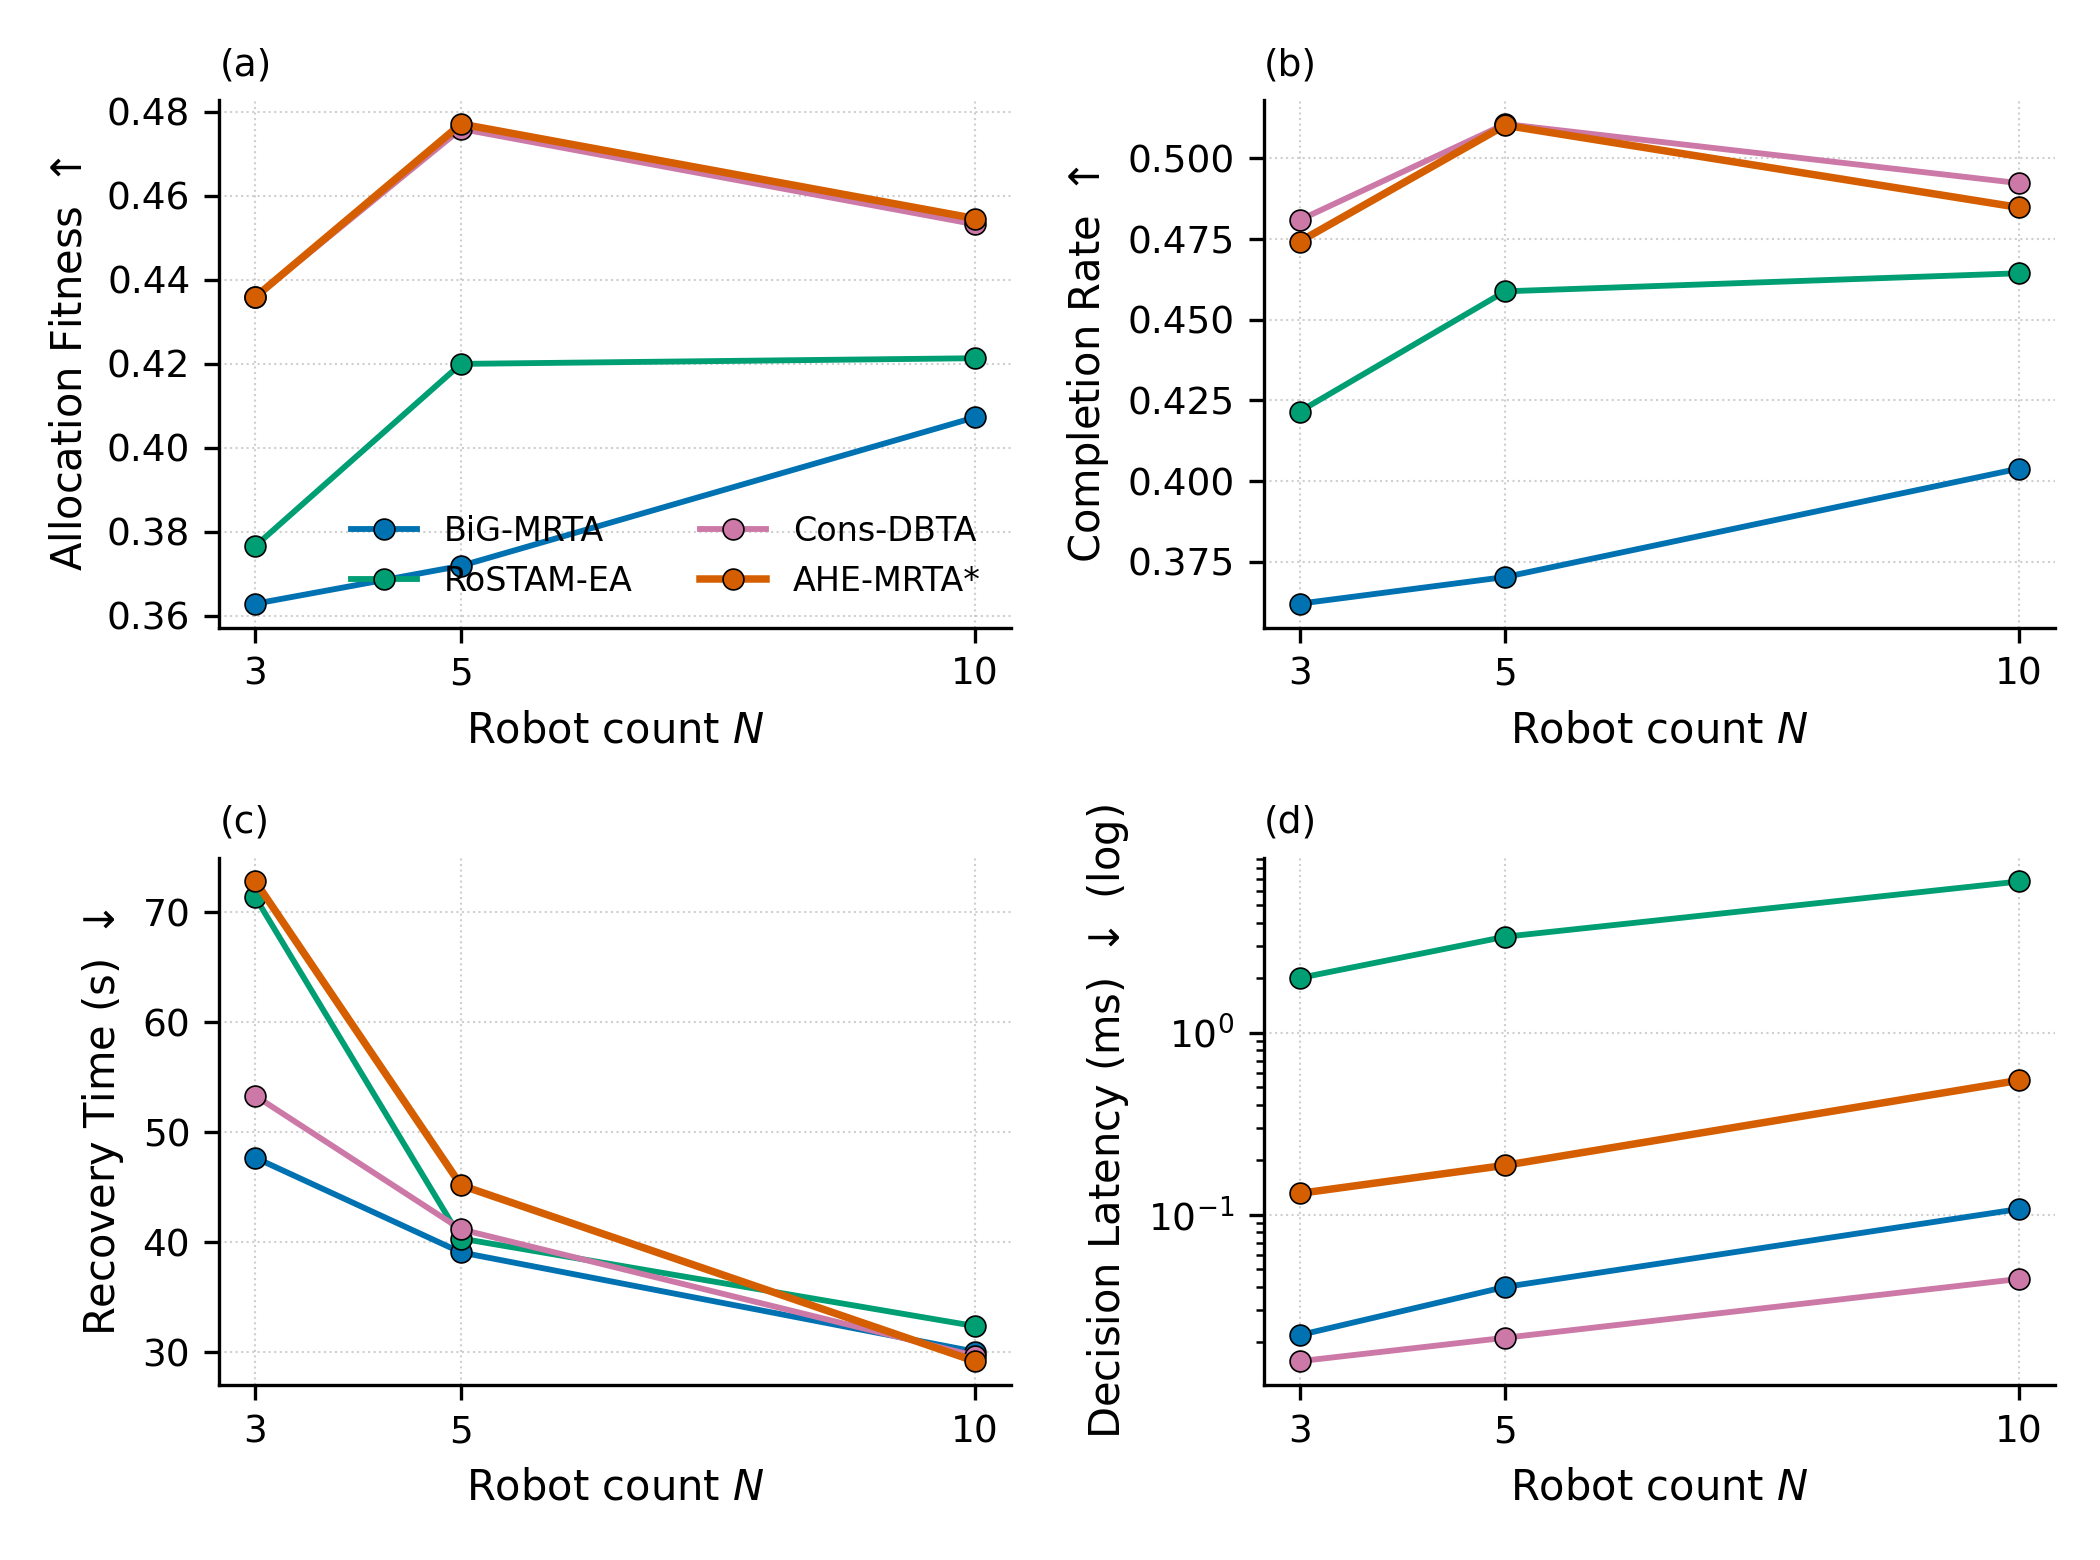
\includegraphics[width=0.92\textwidth]{scalability_panel.png}
  \caption{Stokastik navigasyon vekilinde robot sayısına göre
  ölçeklenebilirlik. Değerler üç senaryoda hücre başına 100 tohumun
  ortalamasıdır: (a) uygunluk, (b) tamamlama oranı, (c) toparlanma süresi ve
  (d) karar gecikmesi. AHE-MRTA her ölçekte uygunlukta en yüksektir. $N=3$, $5$
  ve $10$'da ikinci sıradaki BiG-MRTA'nın sırasıyla $3.3$, $3.6$ ve $2.7$ yüzde
  puanı önündedir ve fark filo büyüdükçe artmaz.}
  \label{fig:scalability}
\end{figure}

\subsection{Kapalı Çevrim Gazebo Değerlendirmesi}
\label{sec:results-gazebo}

Kapalı çevrim Gazebo karşılaştırmasında bütün yöntemler aynı Nav2
parametrelerini, ortamı ve zaman bütçelerini kullanır. Yöntemler yalnızca
tahsis politikası bakımından farklıdır.\footnote{Tablo ve şekillerde,
geodezik ETA kestirimi ile terminal yük onarımı etkin olan yapılandırma
AHE-MRTA* olarak gösterilir (Böl.~\ref{sec:geodesic-repair}).} Kampanya, 3
robot için üç görev yoğunluğu (9/15/24 görev), beş tohum ve toplam 180 deney
içerir. Beş robotlu ölçekte yöntem--senaryo başına 20 tohumla 240, 10 robotlu
ölçekte ise 60 deney yürütülmüştür. Toplam deney sayısı 480'dir. Bütün
yöntemler arası karşılaştırmalarda Bonferroni düzeltmeli Mann--Whitney U testi
uygulanmıştır.

Şekil~\ref{fig:setup-paths}, dört yöntemin aynı \textit{mixed\_stress}
koşusundaki yörüngelerini göstermektedir (5 robot, 25 görev ve tohum 1).
Yörüngeler zemin gerçeği konumlarından yeniden oluşturulmuş ve örneklenen
denetim noktalarıyla birlikte işgal haritasına aktarılmıştır. Bu örnekte
AHE-MRTA ve Consensus-DBTA robotları denetim noktalarına daha geniş biçimde
dağıtırken, tek-atamalı BiG-MRTA daha sınırlı bir alanı kapsamaktadır.

Şekil~\ref{fig:deployment}, üç kıyaslama senaryosunun dışında yürütülen
10-robot/50-görev örnek koşusunun eş zamanlı Gazebo ve RViz görüntülerini
sunmaktadır. Bu koşulda görevler kademeli olarak etkinleşmiş ve arıza
uygulanmamıştır. Gazebo görünümü on TurtleBot3 robotun arenadaki dağılımını,
RViz görünümü ise ortak işgal haritası üzerinde robot konumlarını ve robot
başına Nav2 küresel planlarını göstermektedir. İki panel, filonun tek bir
koridorda yoğunlaşmak yerine her iki şeride dağıldığını göstermektedir.

\begin{figure*}[t]
  \centering
  \begin{minipage}[b]{0.30\textwidth}
    \centering
    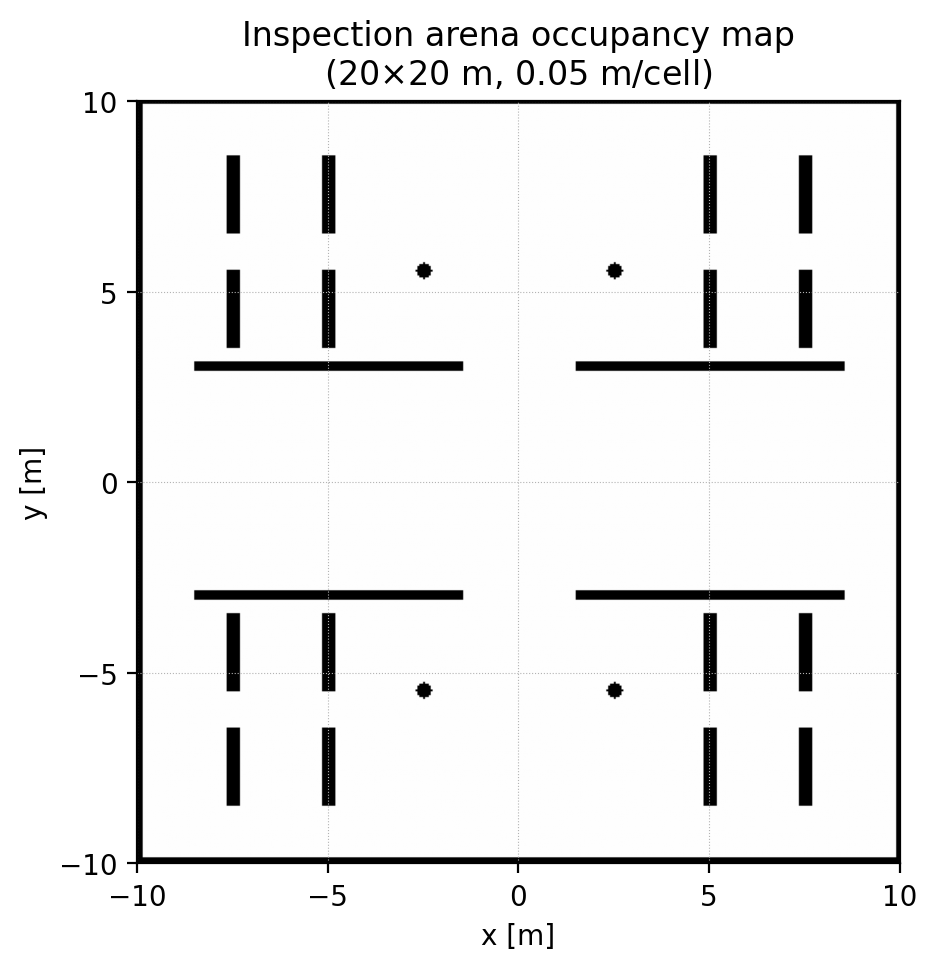
\includegraphics[width=\linewidth]{arena_occupancy_map.png}\\[2pt]
    {\small (a) Nav2 işgal haritası}
  \end{minipage}\hfill
  \begin{minipage}[b]{0.66\textwidth}
    \centering
    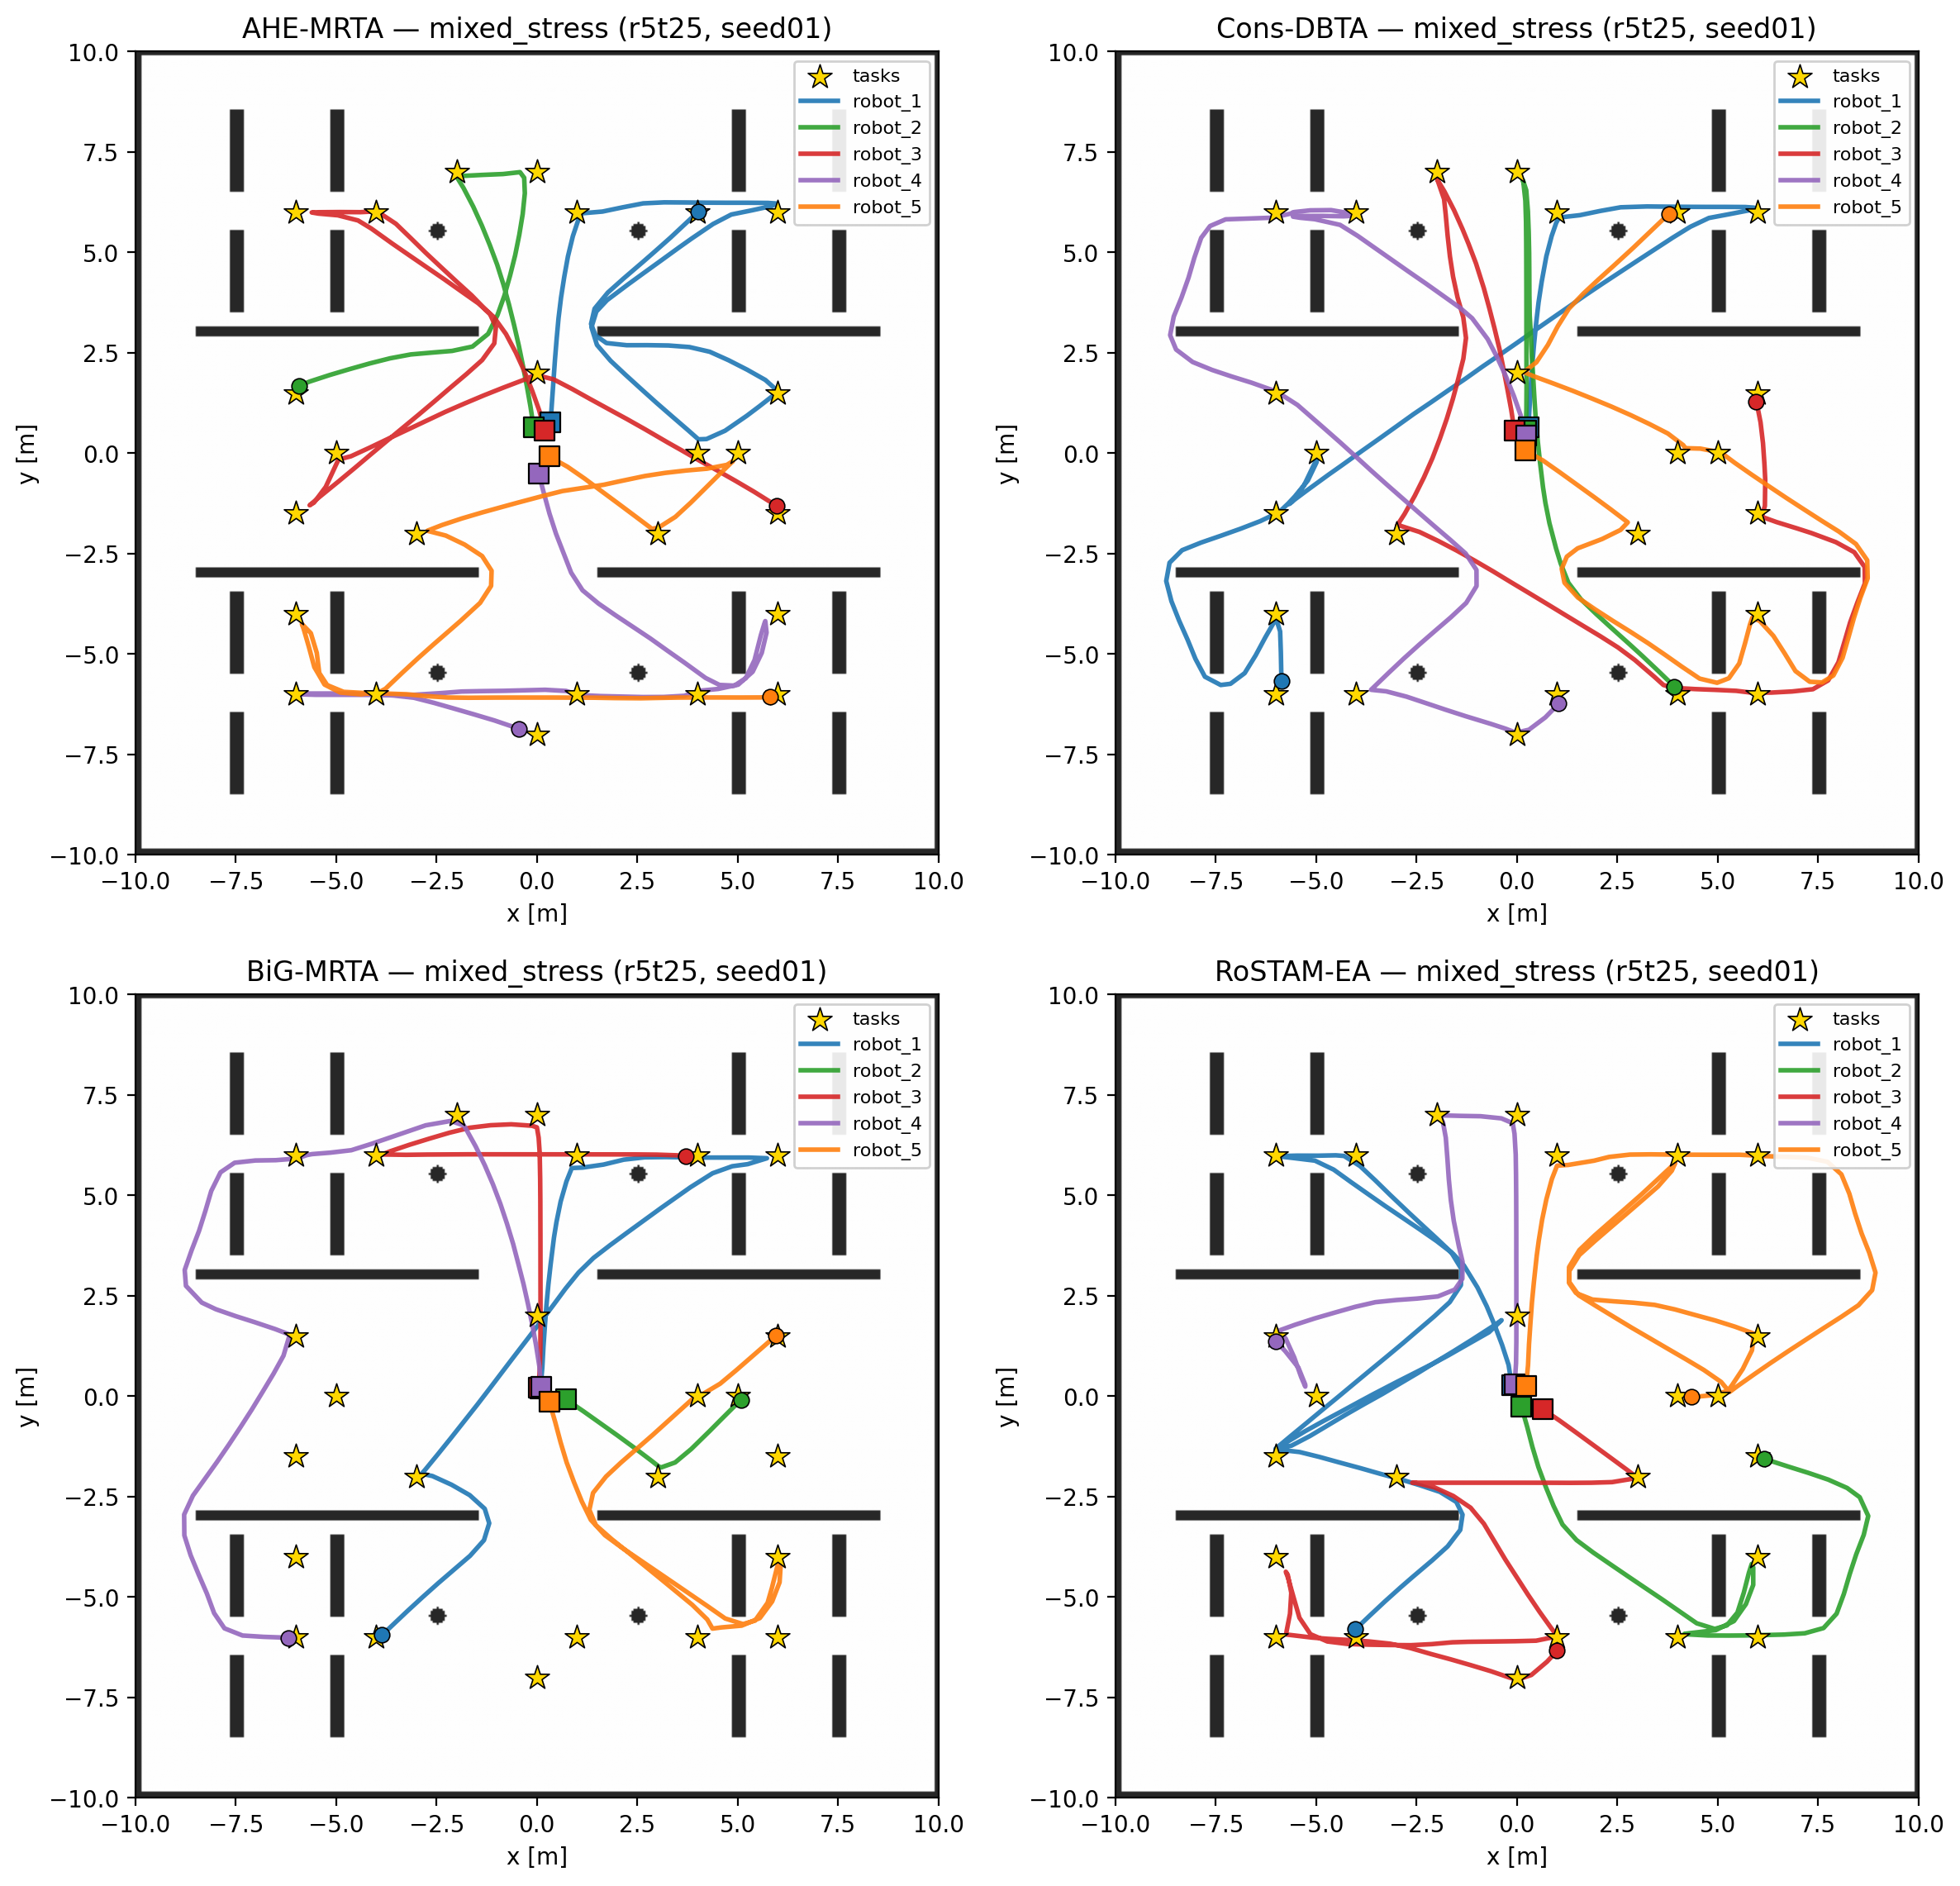
\includegraphics[width=\linewidth]{grid_r5t25_mixed_stress.png}\\[2pt]
    {\small (b) Yürütülen robot yörüngeleri}
  \end{minipage}
  \caption{Deney haritası ve örnek yörüngeler.
  \textbf{(a)} Statik Nav2 işgal haritası (\texttt{obstacle\_map})
  $20\times20$~m boyutunda, 0.05~m hücre çözünürlüğünde ve $[-10,-10]$
  başlangıç noktasındadır. Harita ayırıcı duvarlar, kare sütunlar ve dört
  silindirik engel içerir.
  \textbf{(b)} Tek bir \textit{mixed\_stress} koşusundan (5 robot, 25 görev,
  tohum 1) AHE-MRTA, Consensus-DBTA, BiG-MRTA ve RoSTAM-EA yörüngeleri, sol
  üstten başlayarak okuma sırasıyla verilmiştir. Bunlar,
  Tablo~\ref{tab:main_comparison}'daki 5r/25g
  \textit{mixed\_stress} hücrelerinde kullanılan dört koşudur. Kareler
  başlangıç konumlarını, altın yıldızlar örneklenmiş görev noktalarını, renkli
  eğriler ise zemin gerçeği konumlarından yeniden oluşturulan yolları gösterir.
  Zaman serisi her konumu
  robotun kendi odom çerçevesinde kaydettiği için her yörünge o robotun
  başlangıç konumu kadar ötelenmiştir. Eğrisiz bir kare, başlangıç konumundan
  hiç ayrılmamış
  bir robottur. Burada Consensus-DBTA'nın robot~1'i böyledir. Bu tek koşuluk
  şekil yalnızca niteliksel bir örnektir ve yöntemlerin genel sıralamasını
  göstermez.}
  \label{fig:setup-paths}
\end{figure*}

\begin{figure}[t]
  \centering
  \begin{minipage}[b]{0.495\linewidth}
    \centering
    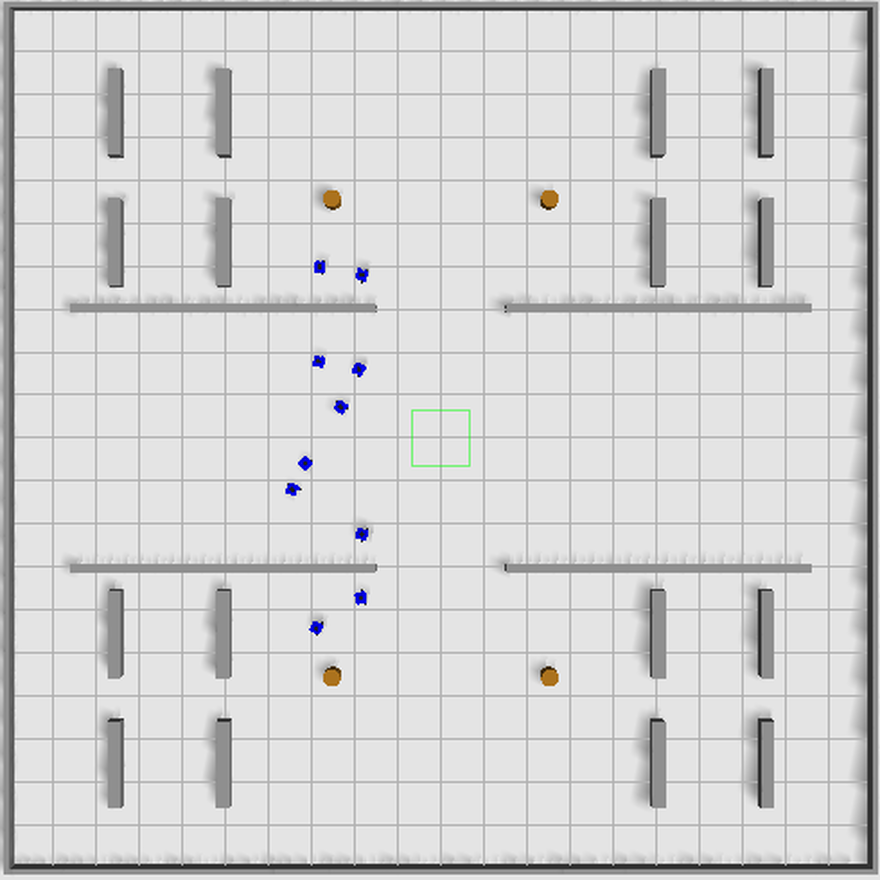
\includegraphics[width=\linewidth]{gazebo_10r_example.png}\\[2pt]
    {\small (a) Gazebo Harmonic --- 3B fizik}
  \end{minipage}\hfill
  \begin{minipage}[b]{0.495\linewidth}
    \centering
    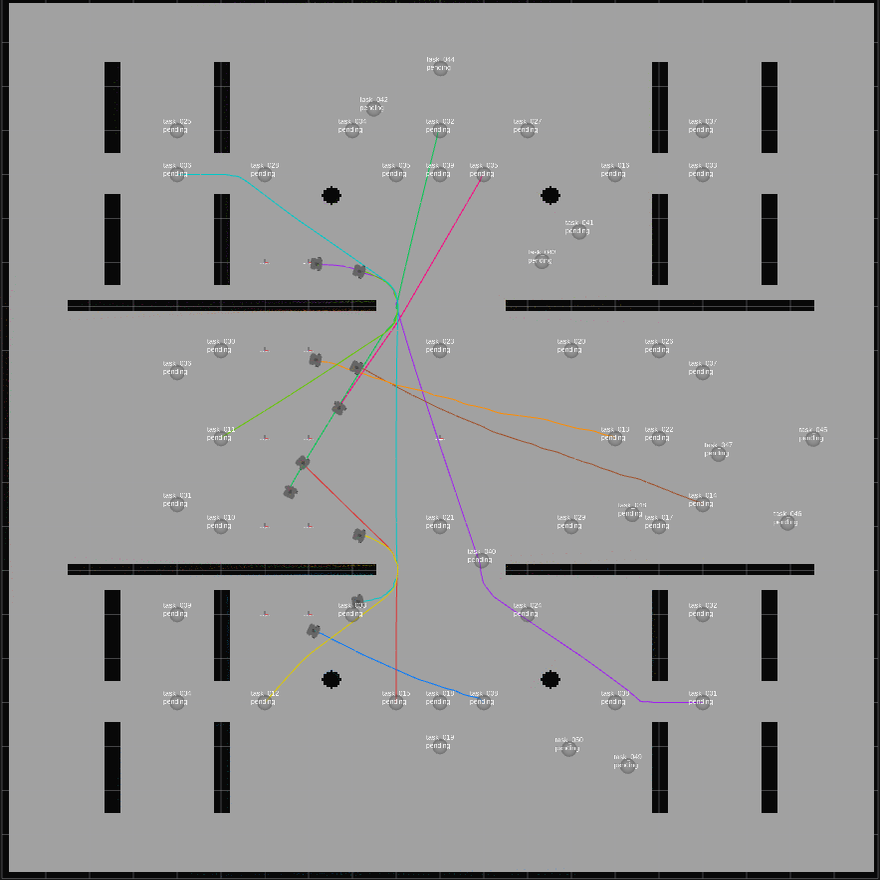
\includegraphics[width=\linewidth]{rviz_10r_example.png}\\[2pt]
    {\small (b) RViz --- harita + canlı Nav2 planları}
  \end{minipage}
  \caption{Üç kıyaslama senaryosunun dışında yürütülen temsilî bir
  10-robot/50-görev AHE-MRTA koşusu. İki panel aynı koşunun aynı durdurulmuş
  simülasyon anını gösterir ve robot konumları iki görünümde örtüşür.
  \textbf{(a)} Gazebo Harmonic (tepeden görünüm): on TurtleBot3
  Waffle\,Pi robotu (mavi) $20{\times}20$~m denetim arenasında---bölme
  duvarları, kare sütunlar ve silindir engeller (turuncu)---atanmış
  denetim noktalarına ilerliyor.
  \textbf{(b)} Eşzamanlı RViz görünümü (paylaşılan harita çerçevesinde):
  önceden oluşturulmuş işgal haritasını, her robotun güncel Nav2 küresel
  planını ve zemin gerçeğine dayalı konumları gösterir. Renk kodlu planlar
  filonun her iki şeride dağıldığını göstermektedir.}
  \label{fig:deployment}
\end{figure}

\begin{table*}[t]
\centering
\caption{Birincil 5-robot/25-görev ölçeğindeki ana karşılaştırma. Her hücre
$n{=}20$ koşu içerir. Senaryo içindeki her sütunun en iyi değeri
\textbf{kalın} gösterilmiştir. AHE-MRTA* ile karşılaştırmada anlamlılık
düzeyleri $^{*}p{<}0.05$, $^{**}p{<}0.01$ ve $^{***}p{<}0.001$'dir.
Mann--Whitney U testlerine her senaryodaki 21 karşılaştırma için Bonferroni
düzeltmesi uygulanmıştır. RecT toparlanma süresini, Kesinti yürütme
kesintisini ve Yen.at. görev başına uygulanan yeniden atama sayısını gösterir.}
\label{tab:main_comparison}
\small
\setlength{\tabcolsep}{3pt}
\begin{tabular}{lrrrrr}
\toprule
\textbf{Yöntem} & \textbf{CR$\uparrow$} & \textbf{Gecikme$\downarrow$(s)} & \textbf{RecT$\downarrow$(s)} & \textbf{Kesinti$\downarrow$} & \textbf{Yen.at.$\downarrow$} \\
\midrule
\multicolumn{6}{l}{\textit{Senaryo: robot\_failure}} \\
\textbf{AHE-MRTA*} & \textbf{1.000 $\pm$ 0.000} & 99.7 $\pm$ 7.6 & 83.7 $\pm$ 43.8 & 0.00 $\pm$ 0.00 & 0.006 $\pm$ 0.015 \\
BiG-MRTA & 0.956$^{***}$ $\pm$ 0.036 & 104.4 $\pm$ 30.1 & \textbf{73.1 $\pm$ 33.9} & 0.00 $\pm$ 0.00 & \textbf{0.004 $\pm$ 0.013} \\
RoSTAM-EA & \textbf{1.000 $\pm$ 0.000} & 92.6 $\pm$ 10.8 & 74.5 $\pm$ 35.8 & 0.00 $\pm$ 0.00 & 0.012 $\pm$ 0.019 \\
Cons-DBTA & \textbf{1.000 $\pm$ 0.000} & \textbf{86.0$^{**}$ $\pm$ 11.2} & 117.9 $\pm$ 29.4 & 0.00 $\pm$ 0.00 & 0.006 $\pm$ 0.015 \\
\midrule
\multicolumn{6}{l}{\textit{Senaryo: mixed\_stress}} \\
\textbf{AHE-MRTA*} & \textbf{1.000 $\pm$ 0.000} & 65.3 $\pm$ 9.1 & 41.9 $\pm$ 17.6 & 0.00 $\pm$ 0.00 & 0.014 $\pm$ 0.020 \\
BiG-MRTA & 0.656$^{***}$ $\pm$ 0.060 & 311.2$^{***}$ $\pm$ 46.1 & \textbf{22.8 $\pm$ 23.7} & 0.00 $\pm$ 0.00 & 0.018 $\pm$ 0.029 \\
RoSTAM-EA & \textbf{1.000 $\pm$ 0.000} & \textbf{61.9 $\pm$ 10.1} & 85.3 $\pm$ 56.0 & 0.00 $\pm$ 0.00 & \textbf{0.002 $\pm$ 0.009} \\
Cons-DBTA & 0.998 $\pm$ 0.009 & 72.8 $\pm$ 16.4 & 81.5 $\pm$ 82.3 & 0.00 $\pm$ 0.00 & 0.032 $\pm$ 0.098 \\
\bottomrule
\end{tabular}
\end{table*}


\begin{table*}[t]
\centering
\caption{Birincil 5-robot/25-görev ölçeğindeki son teslim baskısı
(\textit{deadline\_pressure}) sonuçları. Her hücre $n{=}20$ koşu içerir. DVR,
son teslim ihlal oranını gösterir. Her sütunun en iyi değeri \textbf{kalın}
verilmiştir. AHE-MRTA* ile karşılaştırmada Bonferroni düzeltmeli
Mann--Whitney U testi kullanılmıştır.}
\label{tab:deadline}
\small
\setlength{\tabcolsep}{3pt}
\begin{tabular}{lrrrr}
\toprule
\textbf{Yöntem} & \textbf{CR$\uparrow$} & \textbf{Gecikme$\downarrow$(s)} & \textbf{DVR$\downarrow$} & \textbf{Kesinti$\downarrow$} \\
\midrule
\textbf{AHE-MRTA*} & \textbf{1.000 $\pm$ 0.000} & 78.5 $\pm$ 7.7 & \textbf{0.350 $\pm$ 0.090} & 0.00 $\pm$ 0.00 \\
BiG-MRTA & 0.664$^{***}$ $\pm$ 0.059 & 327.0$^{***}$ $\pm$ 46.5 & 0.402 $\pm$ 0.073 & 0.00 $\pm$ 0.00 \\
RoSTAM-EA & \textbf{1.000 $\pm$ 0.000} & 77.8 $\pm$ 7.3 & 0.498$^{***}$ $\pm$ 0.073 & 0.00 $\pm$ 0.00 \\
Cons-DBTA & \textbf{1.000 $\pm$ 0.000} & \textbf{72.6 $\pm$ 9.3} & 0.422 $\pm$ 0.107 & 0.00 $\pm$ 0.00 \\
\bottomrule
\end{tabular}
\end{table*}


Kapalı çevrimde yöntemler arasındaki en belirgin fark
\textit{deadline\_pressure} senaryosunda ortaya çıkar. Zamanında etkin
tamamlama $\mathrm{CR}{\times}(1{-}\mathrm{DVR})$, AHE-MRTA* için 5 robotta
$0.650$, en güçlü temel yöntem için $0.578$'dir. On robotta karşılık gelen
değerler $0.764$ ve $0.524$'tür. Beş robotlu ölçekte dört yöntemin üçü
görevlerin neredeyse tamamını bitirdiği için fark esas olarak son teslim
ihlal oranından kaynaklanır. AHE-MRTA* için DVR $0.350$, Consensus-DBTA için
$0.422$'dir. Bu fark \%$17$ göreli azalmaya karşılık gelir. On robotta DVR
$0.220$ ve $0.428$ olup göreli azalma \%$49$'dur. Bu sonuçlar, son teslim
baskısı geçersiz kılmasının ve geodezik ETA kestiriminin zaman kısıtının
belirleyici olduğu koşullardaki ortak etkisini yansıtır.

Birincil ölçekte hücre başına $n{=}20$ koşu kullanılmıştır. Yöntemler arası
63 karşılaştırmanın 20'si Bonferroni düzeltmesinden sonra anlamlıdır ve
bunların 15'i AHE-MRTA lehinedir. AHE-MRTA aleyhindeki beş sonuç, üç
senaryonun tamamında tek-atamalı BiG-MRTA'ya ve karışık streste
Consensus-DBTA'ya karşı karar gecikmesi ile robot arızasında Consensus-DBTA'ya
karşı ortalama görev gecikmesidir. On robotlu hücreler $n{=}5$ olduğundan
yalnızca betimleyici olarak yorumlanmıştır.

Tablo~\ref{tab:main_comparison}, birincil ölçekteki \textit{robot\_failure}
ve \textit{mixed\_stress} sonuçlarını göstermektedir. Tablo~\ref{tab:deadline}
ise \textit{deadline\_pressure} sonuçlarını sunmaktadır.
Şekil~\ref{fig:gazebo-multi} aynı ölçeği altı birincil ölçüt üzerinden
özetlemektedir. AHE-MRTA, 5 robotlu ölçekte üç senaryonun tamamında
CR\,=\,1.000'a ulaşır. On robotta CR $0.976$--$0.988$ aralığındadır.
BiG-MRTA'nın son teslim baskısı ve karışık stres koşullarındaki nokta
tahminleri sırasıyla 0.664 ve 0.656'dır. Bununla birlikte dört yöntemli
karşılaştırmada birden çok bileşen aynı anda değiştiği için gözlenen farklar
tek başına seçiciye atfedilemez. Seçicinin etkisi,
Bölüm~\ref{sec:gazebo-ablation}'daki sabit paradigma ve \emph{no-override}
yapılandırmalarını içeren eşleşmiş ablasyonla incelenmiştir.

Kapalı çevrim sonuçları başarım kazanımlarının yürütme maliyetleriyle birlikte
değerlendirilmesi gerektiğini göstermektedir (Bölüm~\ref{sec:discussion}).
\textit{robot\_failure} altında AHE-MRTA'nın ortalama görev gecikmesi 99.7~s,
Consensus-DBTA'nın gecikmesi 86.0~s'dir. Bu karşılaştırma AHE-MRTA aleyhinedir
ve düzeltmeden sonra anlamlı kalır ($p_{\mathrm{adj}}{=}0.002$,
$\delta{=}0.72$). RoSTAM-EA ve tek-atamalı BiG-MRTA için değerler sırasıyla
92.6~s ve 104.4~s'dir. Bu karşılaştırmalar anlamlı değildir. AHE-MRTA'nın
83.7~s'lik arıza toparlanma süresi, Consensus-DBTA'nın 117.9~s değerinden
düşüktür. Ancak RoSTAM-EA'nın 74.5~s ve BiG-MRTA'nın 73.1~s değerlerinden
yüksektir.
Toparlanma süresi karşılaştırmalarının hiçbiri anlamlı değildir
(Şekil~\ref{fig:recovery}). \textit{mixed\_stress} ve
\textit{deadline\_pressure} altında BiG-MRTA 311--327~s ile en yüksek
gecikmeleri gösterir. Ancak bu yöntem daha az görev tamamladığından gecikme
değerleri doğrudan karşılaştırılabilir değildir.

AHE-MRTA'da yürütülen yeniden atama sayısı görev başına ${\leq}0.014$ ve
yürütme kesintisi sıfırdır. Bu ölçüt yalnızca uygulanan yeniden atamaları
saymaktadır. Buna karşılık \texttt{allocation\_instability} sayacı tahsis
edicinin çağrılarını sayar ve bu hücrede AHE-MRTA için 1.02, BiG-MRTA için
5.29 gibi yaklaşık bir mertebe daha büyük değerler üretir. Bu nedenle iki
ölçüt doğrudan karşılaştırılmamalıdır.

Geodezik ETA kestirimcisi yalnızca statik haritaya ve önceden bilinen görev
havuzuna bağlı olduğundan başlangıçta bir kez oluşturulur. Bu yapılandırmada
AHE-MRTA'nın karar gecikmesi 5 robotta 0.81--1.33~ms, 10 robotta
1.9--3.4~ms'dir. Beş robotlu ölçekte tek-atamalı BiG-MRTA'nın gecikmesi
0.14--0.24~ms'dir ve fark üç senaryoda da düzeltmeden sonra anlamlıdır.
AHE-MRTA, \textit{mixed\_stress} altında Consensus-DBTA'dan daha yavaş, diğer
iki senaryoda Consensus-DBTA'dan ve bütün senaryolarda RoSTAM-EA'dan bir veya
iki mertebe daha hızlıdır. AHE-MRTA, BiG-MRTA ve Consensus-DBTA 50~ms karar
bütçesinin içinde kalırken RoSTAM-EA 49--95~ms aralığıyla bu bütçeyi bazı
koşullarda aşmaktadır.

Tablo~\ref{tab:efficiency}, 3-robot ölçeğindeki ikincil verimlilik ölçütlerini
üç yoğunluğun birleştirildiği $n{=}15$ hücreler için raporlar. Karar başına
gecikme AHE-MRTA için 0.47--0.72~ms, BiG-MRTA için 0.08--0.13~ms,
Consensus-DBTA için 0.17--0.51~ms ve RoSTAM-EA için 30.8--48.9~ms'dir.
Birincil 5-robot ölçeğinde karşılık gelen aralıklar sırasıyla 0.81--1.33~ms,
0.14--0.24~ms, 0.45--2.43~ms ve 49--95~ms'dir. AHE-MRTA bütün ölçeklerde
50~ms karar bütçesinin içinde kalırken RoSTAM-EA bazı koşullarda bu bütçeyi
aşar. Birincil ölçekte 60 AHE-MRTA koşusunda kaydedilen 1{,}628 kararın en
yavaşı 4.35~ms sürmüş ve hiçbir karar zaman bütçesini aşmamıştır.
\footnote{Birincil 5-robot kampanyası geodezik kestirimci başlangıçta
oluşturularak yürütüldüğünden raporlanan AHE-MRTA gecikmesi doğrudan kampanya
verisidir. Üç ve 10 robotlu AHE-MRTA gecikmeleri, özgün hücrelerle bire bir
eşleşen 60 koşuluk yeniden ölçümden elde edilmiştir (dört ölçek--yoğunluk
hücresi $\times$ üç senaryo $\times$ beş tohum). Diğer AHE-MRTA ölçütleri ile
temel yöntemlerin bütün ölçütleri özgün kampanyadan alınmıştır. Haritadan
türetilen kurulumun zamanlanan karar yolundan çıkarılması, tahsis kararlarını
bit düzeyinde değiştirmemiştir. 5r/25t eşlenik kontrolünde değiştirilmemiş
yapılandırma önceki kampanya gecikmesini yeniden üretmiştir (15.4 ve 15.9~ms).
Gecikme dışındaki farklar olağan Gazebo koşuları arası değişim içinde
kalmıştır.}
Tek-atamalı uzlaşma yöntemleri yüksek iş yükü dengesi ve düşük mesaj sayısı
sağlamaktadır. Üç robotta bütün robotlar için Jain dengesi AHE-MRTA'da
0.85--0.99, BiG-MRTA'da 0.93--0.96 ve Consensus-DBTA'da 0.88--1.00
aralığındadır. AHE-MRTA'nın toplam yol uzunluğu da 44--104~m yerine
99--113~m'dir. Bu artış, yeniden atanan görevlere farklı robotların yönelmesiyle
ilişkilidir.

\begin{table}[t]
\centering
\caption{Verimlilik metrikleri (Gazebo, 3 robot, 15 g\"orev, 5 tohum). WLBal: Jain i\c{s} y\"uk\"u dengesi; Lat: ortalama karar gecikmesi; Msgs: tahsis mesajlar\i; Dist: toplam yol mesafesi.}
\label{tab:efficiency}
\small
\begin{tabular}{lrrrr}
\toprule
\textbf{Method} & \textbf{WLBal$\uparrow$} & \textbf{Lat$\downarrow$(ms)} & \textbf{Msgs$\downarrow$} & \textbf{Dist$\downarrow$(m)} \\
\midrule
\multicolumn{5}{l}{\textit{Senaryo: robot\_failure}} \\
\textbf{AHE-MRTA*} & 0.281 & 0.18 & 38 & 122.5 \\
BiG-MRTA & 0.481 & \textbf{0.12} & 121 & \textbf{71.3} \\
RoSTAM-EA & \textbf{0.550} & 31.05 & \textbf{2} & 83.3 \\
Cons-DBTA & 0.465 & 0.23 & 11 & 89.1 \\
\midrule
\multicolumn{5}{l}{\textit{Senaryo: mixed\_stress}} \\
\textbf{AHE-MRTA*} & 0.268 & 0.21 & 33 & 110.1 \\
BiG-MRTA & \textbf{0.629} & \textbf{0.08} & 177 & \textbf{59.5} \\
RoSTAM-EA & 0.479 & 25.64 & \textbf{4} & 92.9 \\
Cons-DBTA & 0.309 & 0.13 & 10 & 103.0 \\
\midrule
\multicolumn{5}{l}{\textit{Senaryo: deadline\_pressure}} \\
\textbf{AHE-MRTA*} & 0.733 & 0.23 & 26 & 103.0 \\
BiG-MRTA & 0.719 & \textbf{0.08} & 181 & \textbf{42.2} \\
RoSTAM-EA & 0.666 & 42.46 & \textbf{1} & 78.4 \\
Cons-DBTA & \textbf{0.819} & 0.36 & 6 & 81.7 \\
\bottomrule
\end{tabular}
\end{table}


Tablo~\ref{tab:effectsize}, düzeltilmiş testlerle birlikte Cliff $\delta$
etki büyüklüklerini verir. İşaretler $\delta{>}0$ AHE-MRTA lehine olacak
biçimde düzenlenmiştir. BiG-MRTA'ya karşı tamamlama etkisi
\textit{mixed\_stress} ve \textit{deadline\_pressure} için
$\delta{=}{+}1.00$, \textit{robot\_failure} için ${+}0.70$'tir. Robot arızası
altında son teslim uyumu etkileri üç temel yönteme karşı ${+}0.83$--${+}0.86$
aralığındadır ve düzeltmeden sonra anlamlıdır. Son teslim baskısında yalnızca
RoSTAM-EA karşılaştırması hem büyük hem anlamlıdır (${+}0.81$). BiG-MRTA ve
Consensus-DBTA karşılaştırmaları sırasıyla ${+}0.34$ ve ${+}0.39$'dur.
En büyük AHE-MRTA aleyhine etki, karışık streste tek-atamalı BiG-MRTA'ya karşı
toparlanma süresinde gözlenir (${-}0.50$), ancak düzeltmeden sonra anlamlı
değildir. Robot arızasında Consensus-DBTA'ya karşı toparlanma etkisi ters
yöndedir (${+}0.45$). Düzeltilmiş yeniden atama ölçütünde hiçbir karşılaştırma
$|\delta|{=}0.30$'u aşmaz. Bu sonuçlar en belirgin farkın son teslim uyumunda
olduğunu, yürütme maliyetlerindeki farkların ise çoğunlukla küçük kaldığını
göstermektedir.

\begin{table}[t]
\centering
\caption{AHE-MRTA* ile her temel yöntem arasındaki birincil ölçütler için Cliff
$\delta$ etki büyüklükleri. Pozitif $\delta$, AHE-MRTA* lehine farkı gösterir.
Anlamlılık düzeyleri $^{*}p{<}0.05$, $^{**}p{<}0.01$ ve
$^{***}p{<}0.001$'dir. Değerler Bonferroni düzeltmeli Mann--Whitney U
testlerine dayanır.
CR tamamlama oranını, DVR son teslim ihlal oranını, RecT toparlanma süresini ve
Yen.at. görev başına uygulanan yeniden atama sayısını gösterir.}
\label{tab:effectsize}
\small
\begin{tabular}{llrrr}
\toprule
\textbf{Ölçüt} & \textbf{Etki} & \textbf{BiG} & \textbf{RoSTAM} & \textbf{Cons-DBTA} \\
\midrule
\multicolumn{5}{l}{\textit{Senaryo: robot\_failure}} \\
CR & $\delta$ & +0.70*** & +0.00 & +0.00 \\
DVR & $\delta$ & +0.83*** & +0.86*** & +0.85*** \\
RecT & $\delta$ & -0.08 & -0.09 & +0.45 \\
Yen.at. & $\delta$ & -0.04 & +0.15 & -0.00 \\
\midrule
\multicolumn{5}{l}{\textit{Senaryo: mixed\_stress}} \\
CR & $\delta$ & +1.00*** & +0.00 & +0.05 \\
DVR & $\delta$ & -0.03 & +0.47 & +0.65** \\
RecT & $\delta$ & -0.50 & +0.49 & +0.18 \\
Yen.at. & $\delta$ & +0.06 & -0.30 & -0.03 \\
\midrule
\multicolumn{5}{l}{\textit{Senaryo: deadline\_pressure}} \\
CR & $\delta$ & +1.00*** & +0.00 & +0.00 \\
DVR & $\delta$ & +0.34 & +0.81*** & +0.39 \\
RecT & $\delta$ & -0.00 & -0.00 & -0.00 \\
Yen.at. & $\delta$ & -0.00 & -0.00 & -0.00 \\
\bottomrule
\end{tabular}
\\[2pt]\footnotesize $|\delta|{>}0.47$ büyük etkiyi gösterir.
\end{table}


Birincil 5-robot ölçeğinde hücre başına $n{=}20$ koşuyla yapılan 63
karşılaştırmanın 20'si Bonferroni düzeltmesinden sonra anlamlıdır. Bunların
15'i AHE-MRTA lehine, 5'i aleyhinedir. Yirmi sekiz karşılaştırmada düzeltilmemiş
$p{<}0.05$ elde edilmiştir. AHE-MRTA lehindeki sonuçlar, ilgili temel
yöntemlere karşı tamamlama oranı ve son teslim ihlal oranı ile RoSTAM-EA ve
Consensus-DBTA'ya karşı karar gecikmesini içerir. Aleyhteki sonuçlar, üç
senaryoda tek-atamalı BiG-MRTA'ya karşı karar gecikmesi, karışık streste
Consensus-DBTA'ya karşı karar gecikmesi ve robot arızasında Consensus-DBTA'ya
karşı ortalama görev gecikmesidir. Üç robotlu ölçekte hücre başına $n{=}15$
koşuyla yapılan 63 karşılaştırmanın 14'ü anlamlıdır ve bunların 8'i AHE-MRTA
lehinedir. On robotlu ölçekte hücre başına beş tohum bulunmaktadır. Bu örneklem
büyüklüğünde ulaşılabilen en küçük iki yönlü Mann--Whitney değeri
${\approx}0.008$, düzeltilmiş eşik ise $0.05/21{\approx}0.0024$ olduğundan
hiçbir karşılaştırma anlamlılık eşiğini geçemez. Bu hücreler bu nedenle
betimleyicidir. En yüksek istatistiksel güce sahip yöntemler arası deney,
500-tohumlu navigasyon vekilidir (Bölüm~\ref{sec:results-sim}). Gazebo
karşılaştırması yalnızca birincil ölçekte düzeltilmiş çıkarımı destekler.

On robotlu Gazebo kampanyasındaki 60 deney eksiksiz tamamlanmıştır
(Şekil~\ref{fig:gazebo-10r}). AHE-MRTA her senaryoda en yüksek veya eşit en
yüksek tamamlama oranına ulaşır (CR\,=\,0.976--0.988). Son teslim baskısında
CR\,=\,0.980 ve DVR\,=\,0.220 ile zamanında etkin tamamlama yaklaşık
$0.76$'dır. Consensus-DBTA ve RoSTAM-EA için karşılık gelen değerler yaklaşık
$0.52$ ve $0.48$'dir. Bu yöntemler CR\,=\,0.916/0.964 ve
DVR\,=\,0.428/0.504 düzeyindedir. Karışık streste AHE-MRTA en yüksek
tamamlama oranını elde eder (CR\,=\,0.988), ancak Consensus-DBTA zamanında
etkin tamamlamada $0.650$ ile AHE-MRTA'nın $0.641$ değerini geçer. Her iki
yöntem de RoSTAM-EA'nın $0.529$ değerinin üzerindedir. Robot arızasında
AHE-MRTA ile tek-atamalı BiG-MRTA CR\,=\,0.976 ile eşittir. Zamanında etkin
tamamlamada BiG-MRTA $0.936$, AHE-MRTA $0.915$ elde eder. BiG-MRTA'nın diğer
iki senaryodaki düşük DVR değeri, daha düşük tamamlamayla birlikte
değerlendirilmelidir (CR\,=\,0.696--0.724).

Beş robotlu ölçekte AHE-MRTA üç senaryoda da CR\,=\,1.000'a ulaşır. Zamanında
etkin tamamlama robot arızasında $0.986$ (DVR\,=\,0.014) ve temel yöntemlerde
${\leq}0.890$'dır. Son teslim baskısında bu değer $0.650$ (DVR\,=\,0.350),
temel yöntemlerde ise en fazla $0.578$'dir. Karışık streste AHE-MRTA için
$0.616$, temel yöntemlerde ise en fazla $0.542$ elde edilmiştir. BiG-MRTA'nın
karışık stres ve son teslim baskısındaki
tamamlama oranları CR\,=\,0.656/0.664'tür. Karar gecikmesi 5 robotta
0.81--1.33~ms, 10 robotta 1.9--3.4~ms'dir. On robotta 48--107~ms gecikmeye
ulaşan RoSTAM-EA ile karşılaştırıldığında AHE-MRTA $20$--$82{\times}$ daha
hızlıdır ve iki ölçekte de gerçek zaman bütçesi içinde kalır.

Şekil~\ref{fig:dom-recovery}, 3-robot ölçeğinde \textit{robot\_failure}
altındaki baskınlık durumunu, tohum ortalamalı tamamlama eğrisini ve toparlanma
süresi ile gecikmenin koşular arası dağılımını göstermektedir. Yeniden atama
medyanı dört yöntemde de sıfırdır. Sıfırdan farklı değerler AHE-MRTA ve
Consensus-DBTA için 15 koşunun 2'sinde, BiG-MRTA için 4'ünde görülmüş,
RoSTAM-EA'da görülmemiştir. Tek bir koşudaki en yüksek değer AHE-MRTA için
görev başına $0.11$, Consensus-DBTA için $0.30$'dur. Şekil~\ref{fig:timeline},
\textit{robot\_failure} ve \textit{mixed\_stress} için kümülatif tamamlama
eğrilerini sunmaktadır.

\begin{figure}[t]
  \centering
  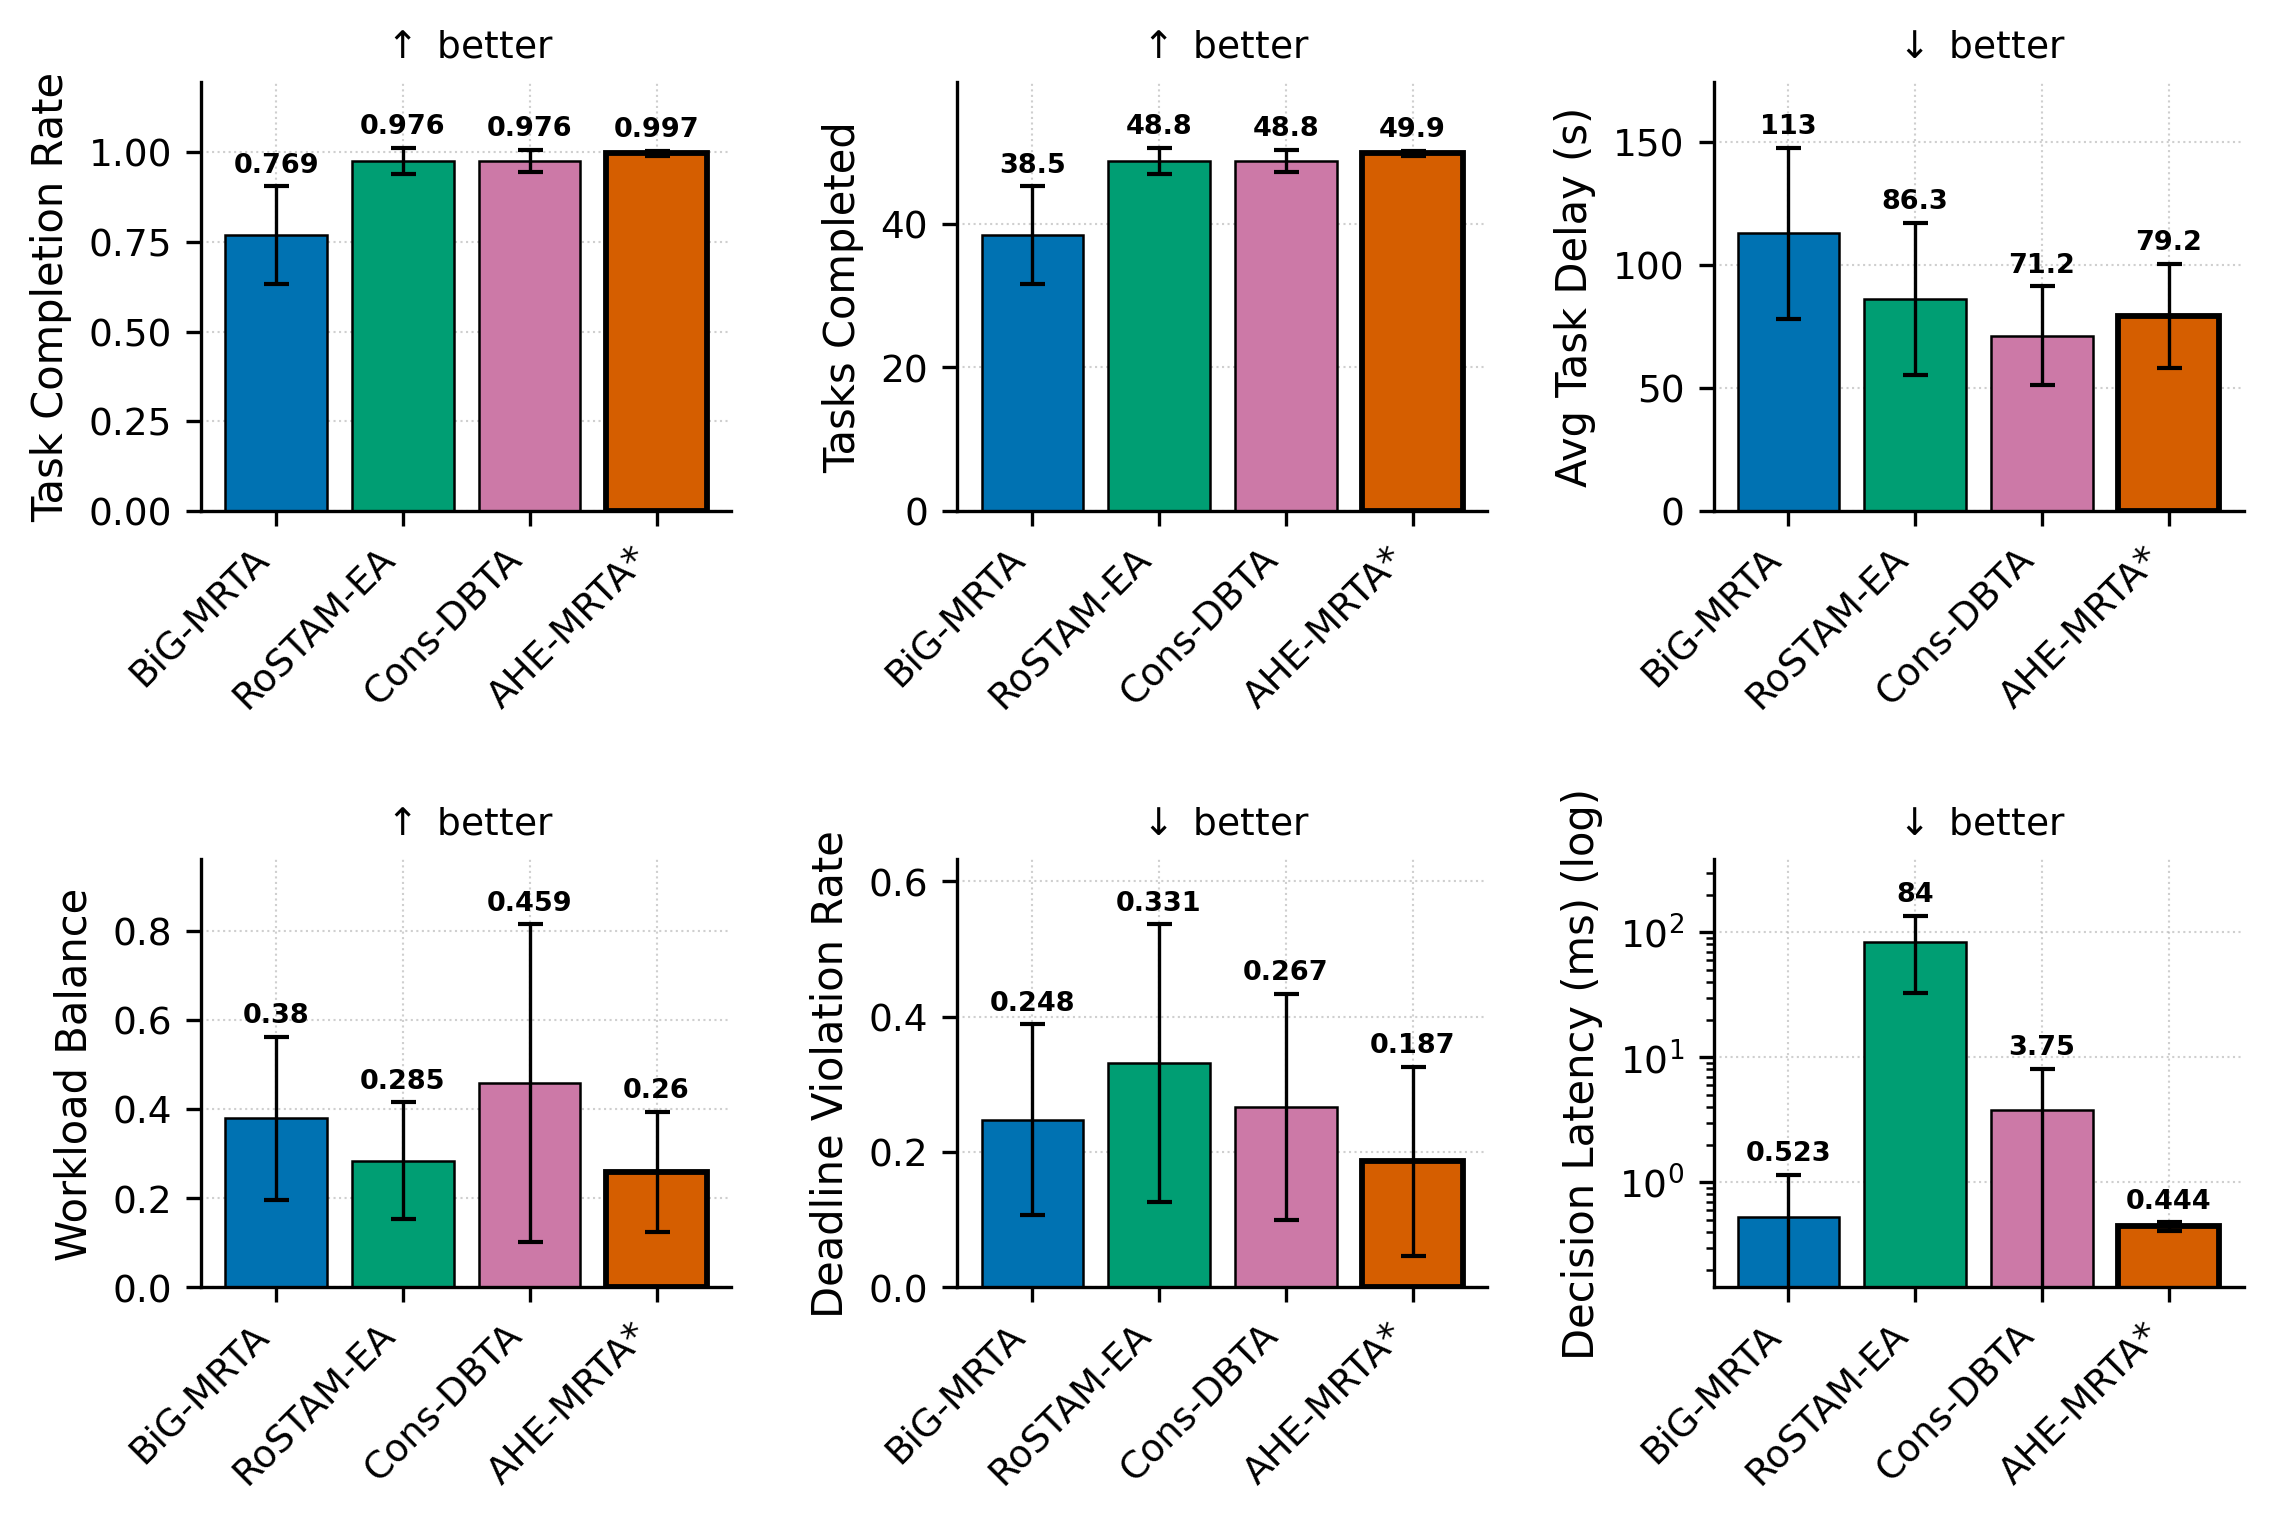
\includegraphics[width=\textwidth]{baseline_comparison_10r.png}
  \caption{10-robot ölçeğinde çok-metrikli karşılaştırma. Toplam 60 deney,
  4 yöntem $\times$ 3 senaryo $\times$ 5 tohum biçiminde yürütülmüştür.
  Üç senaryo havuzlandığı için her çubuk $n{=}15$ koşuyu ve ortalama $\pm$
  standart sapmayı gösterir. Karar gecikmesi logaritmik ölçektedir. Senaryolar
  üzerinden havuzlandığında AHE-MRTA tamamlamada
  (0.799--0.952'ye karşı 0.981) ve zamanında-etkin tamamlamada
  $\mathrm{CR}{\times}(1{-}\mathrm{DVR})$ (0.587--0.690'a karşı 0.773) öndedir,
  son teslim ihlalinde en düşüktür
  (0.224--0.367'ye karşı 0.212). Ortalama karar gecikmesi ise tek-atamalı
  BiG-MRTA'nın 0.6~ms'sine, Consensus-DBTA'nın 1.8~ms'sine ve RoSTAM-EA'nın
  69.1~ms'sine karşı 2.6~ms'dir. Havuzlanmış değerler, farkın esas olarak
  \textit{deadline\_pressure} senaryosunda oluştuğunu doğrudan göstermez.
  Bu senaryoda AHE-MRTA için DVR 0.220, diğer yöntemler için
  0.296--0.504'tür. Senaryo başına $n{=}5$ olan yöntemler arası hücreler
  betimleyicidir ve düzeltilmiş bir yöntem sıralamasını desteklemez.}
  \label{fig:gazebo-10r}
\end{figure}

\begin{figure}[t]
  \centering
  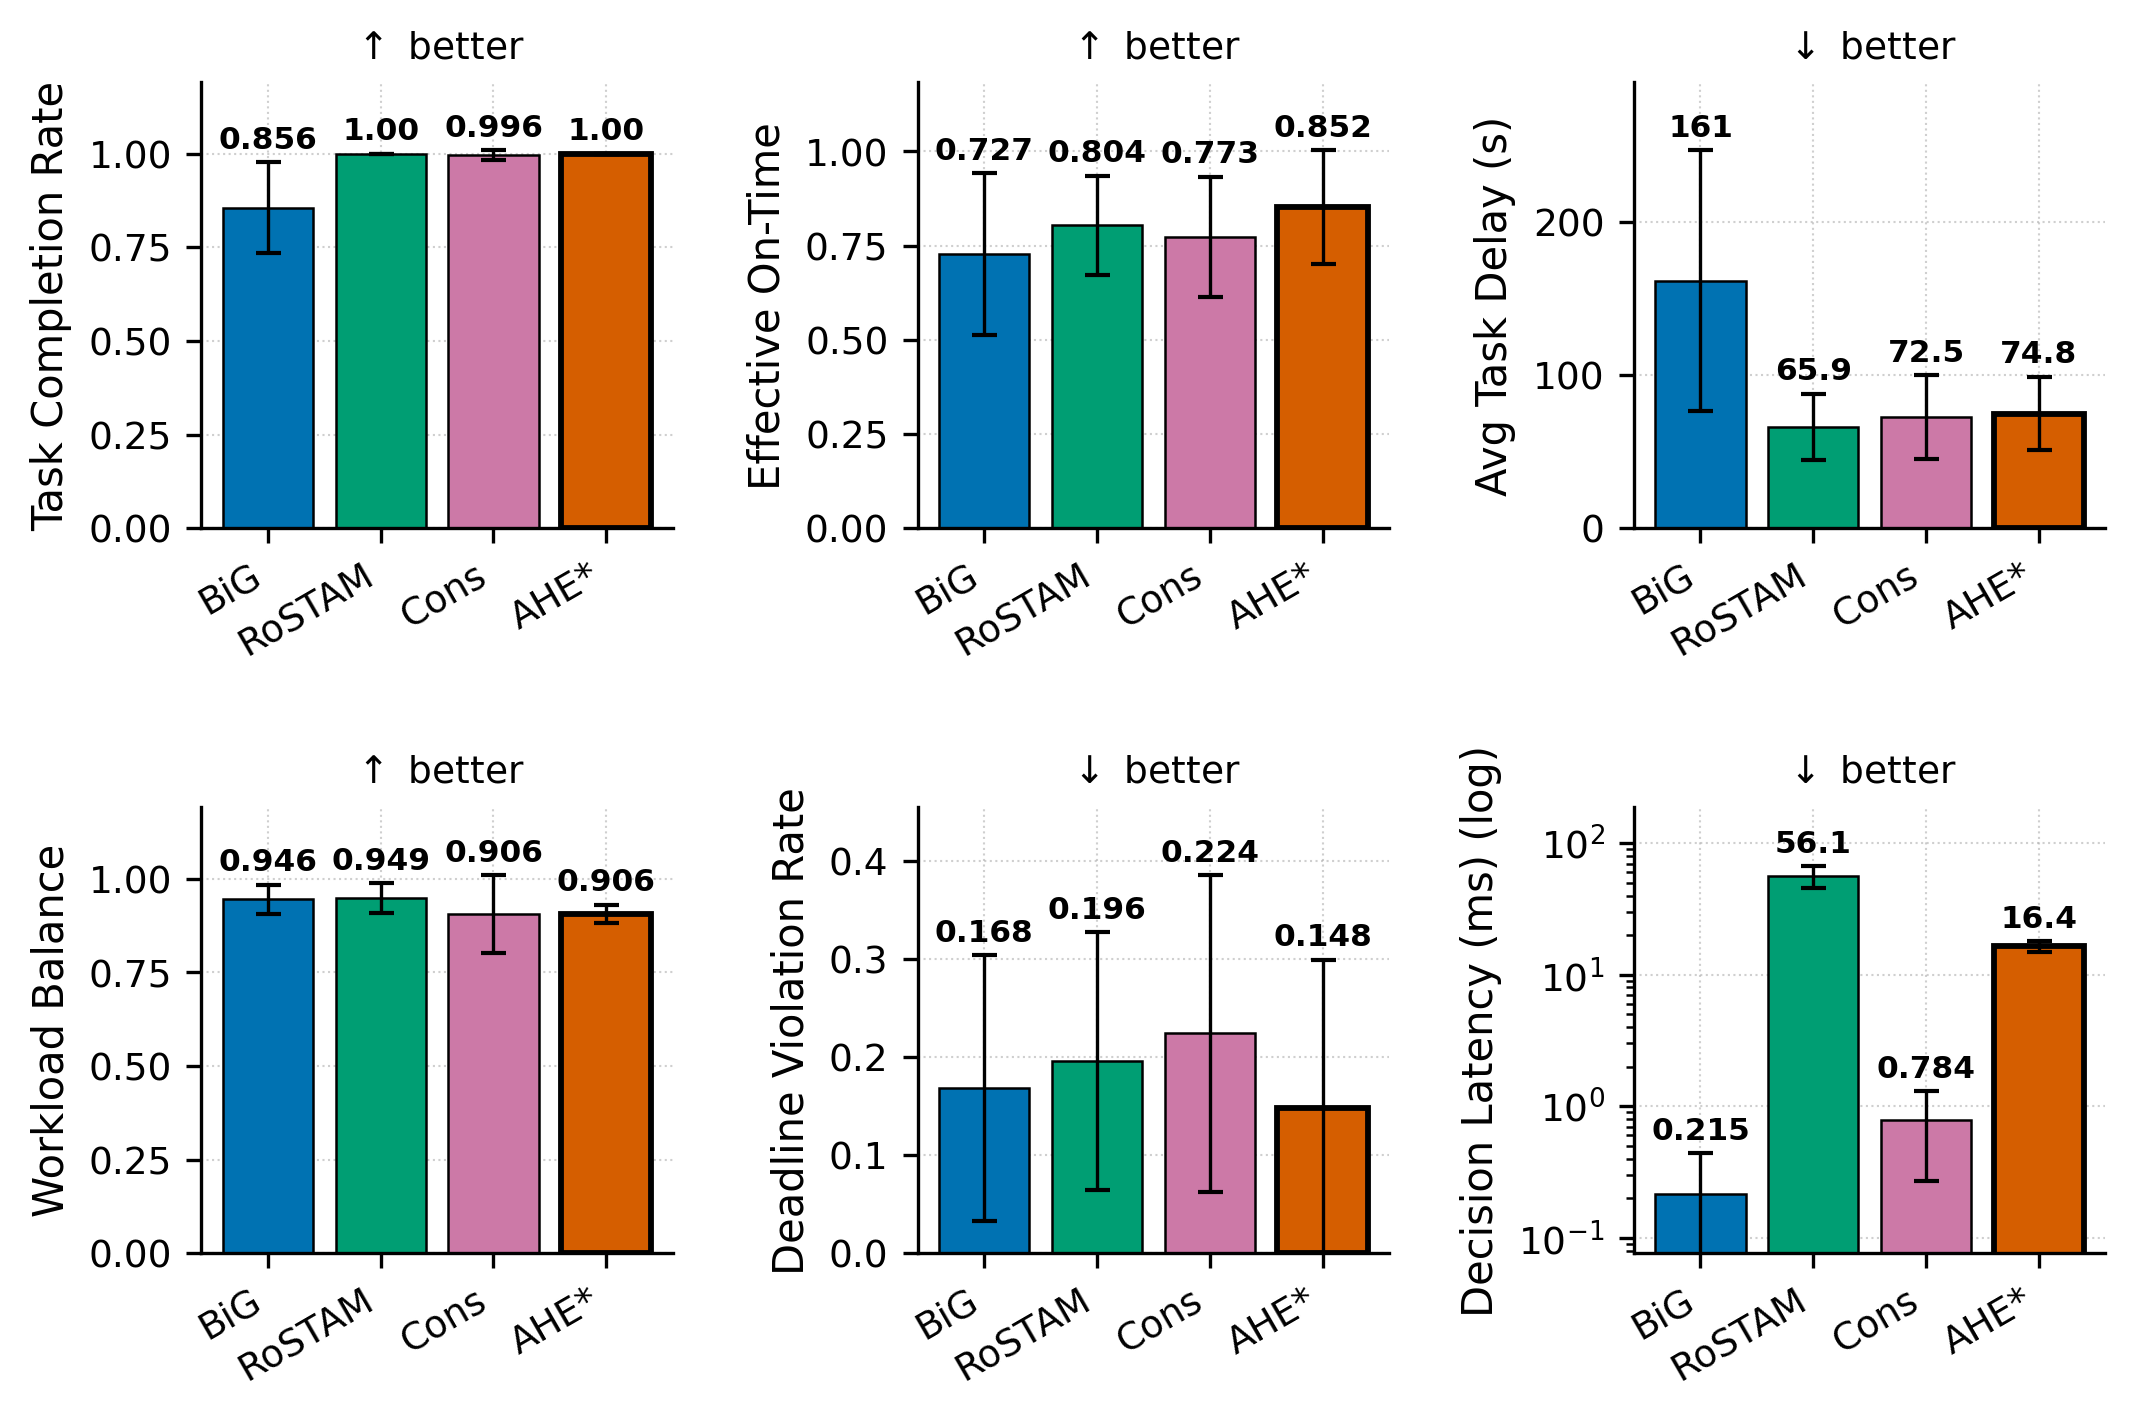
\includegraphics[width=\textwidth]{baseline_comparison_multi_metric.png}
  \caption{Birincil 5-robot/25-görev ölçeğinde çok ölçütlü karşılaştırma.
  \textit{robot\_failure} ve \textit{mixed\_stress} senaryoları gösterim
  amacıyla birleştirilmiştir. Her yöntem--senaryo hücresinde $n{=}20$ tohum
  bulunur ve çubuklar ortalama $\pm$ standart sapmayı gösterir. Ölçütler
  tamamlama oranı, zamanında etkin tamamlama
  $\mathrm{CR}{\times}(1{-}\mathrm{DVR})$, ortalama gecikme, Jain iş yükü
  dengesi, son teslim ihlal oranı ve logaritmik ölçekte karar gecikmesidir.
  AHE-MRTA CR\,=\,1.000 ve $0.801$ zamanında etkin tamamlama elde eder. Diğer
  yöntemlerde ikinci ölçüt $0.647$--$0.716$ aralığındadır. BiG-MRTA'nın düşük
  DVR değeri en düşük tamamlama oranıyla birlikte değerlendirilmelidir.
  AHE-MRTA'nın reaktif yeniden tahsisi daha yüksek gecikme ve rota maliyetiyle
  ilişkilidir. Düzeltilmiş testler her senaryoda ayrı yürütülmüş ve metinde
  raporlanmıştır.}
  \label{fig:gazebo-multi}
\end{figure}

\begin{figure}[t]
  \centering
  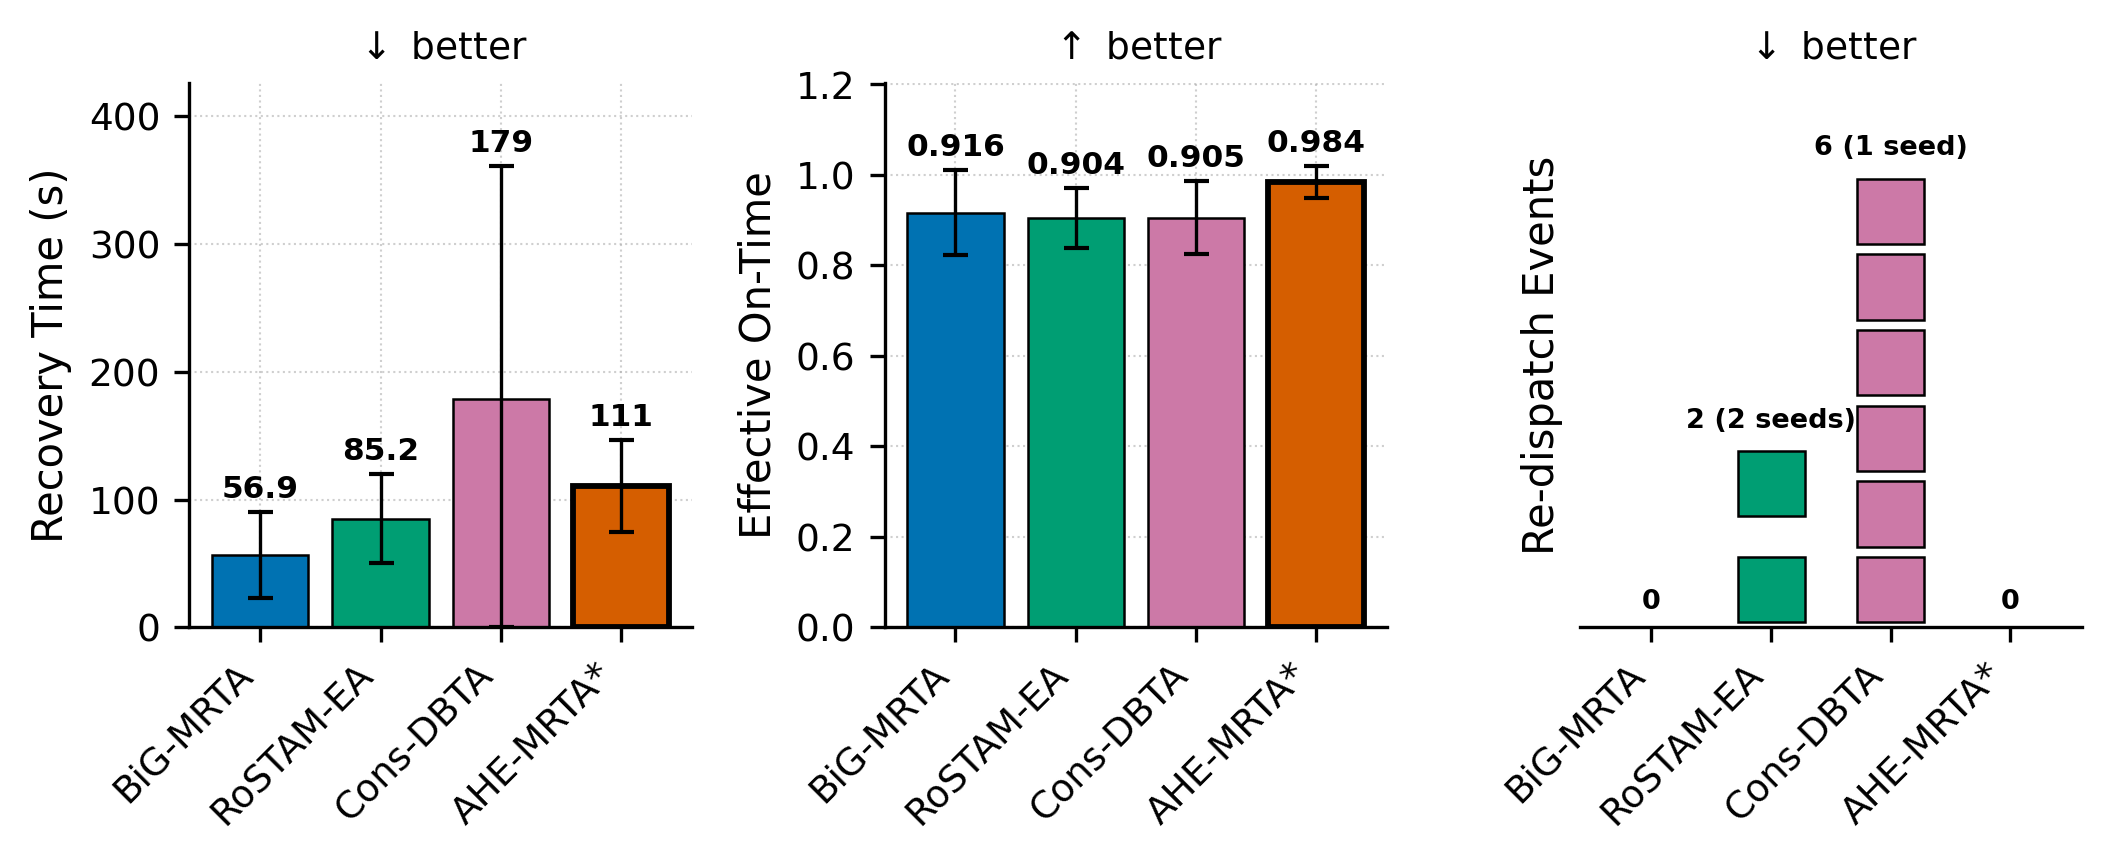
\includegraphics[width=\textwidth]{failure_recovery.png}
  \caption{Birincil 5-robot/25-görev ölçeğinde \textit{robot\_failure}
  altındaki toparlanma davranışı ($n{=}20$ tohum). Toparlanma süresi ve
  zamanında etkin tamamlama $\mathrm{CR}{\times}(1{-}\mathrm{DVR})$ için
  çubuklar ortalama $\pm$ standart sapmayı gösterir. Negatif değer mümkün
  olmadığından hata çubukları sıfırda sınırlandırılmıştır. Yeniden atamalar
  birim çubuklarla gösterilmiş ve farklı tohumlar boşlukla ayrılmıştır. Seksen
  koşunun 66'sında yeniden atama yoktur. Kalan 14 koşunun her birinde bir olay
  vardır. Bu olayların üçü AHE-MRTA, ikisi BiG-MRTA, üçü Consensus-DBTA ve
  altısı RoSTAM-EA koşularındadır. Bütün yöntemlerde yürütme kesintisi sıfır
  olduğundan gösterilmemiştir. Toparlanma süresi karşılaştırmalarının hiçbiri
  düzeltmeden sonra anlamlı değildir. En küçük ham değer Consensus-DBTA
  karşılaştırmasındadır. AHE-MRTA ve Consensus-DBTA için süreler 83.7~s ve
  117.9~s, ham $p{=}0.017$ ve düzeltilmiş $p{=}0.35$'tir. Ham tamamlama oranı
  AHE-MRTA, RoSTAM-EA ve Consensus-DBTA için $1.000$ olduğundan ayırt edici
  değildir. Zamanında etkin tamamlama AHE-MRTA için $0.986$, diğer iki yöntem
  için $0.884$--$0.890$'dır.}
  \label{fig:recovery}
\end{figure}

\begin{figure}[t]
  \centering
  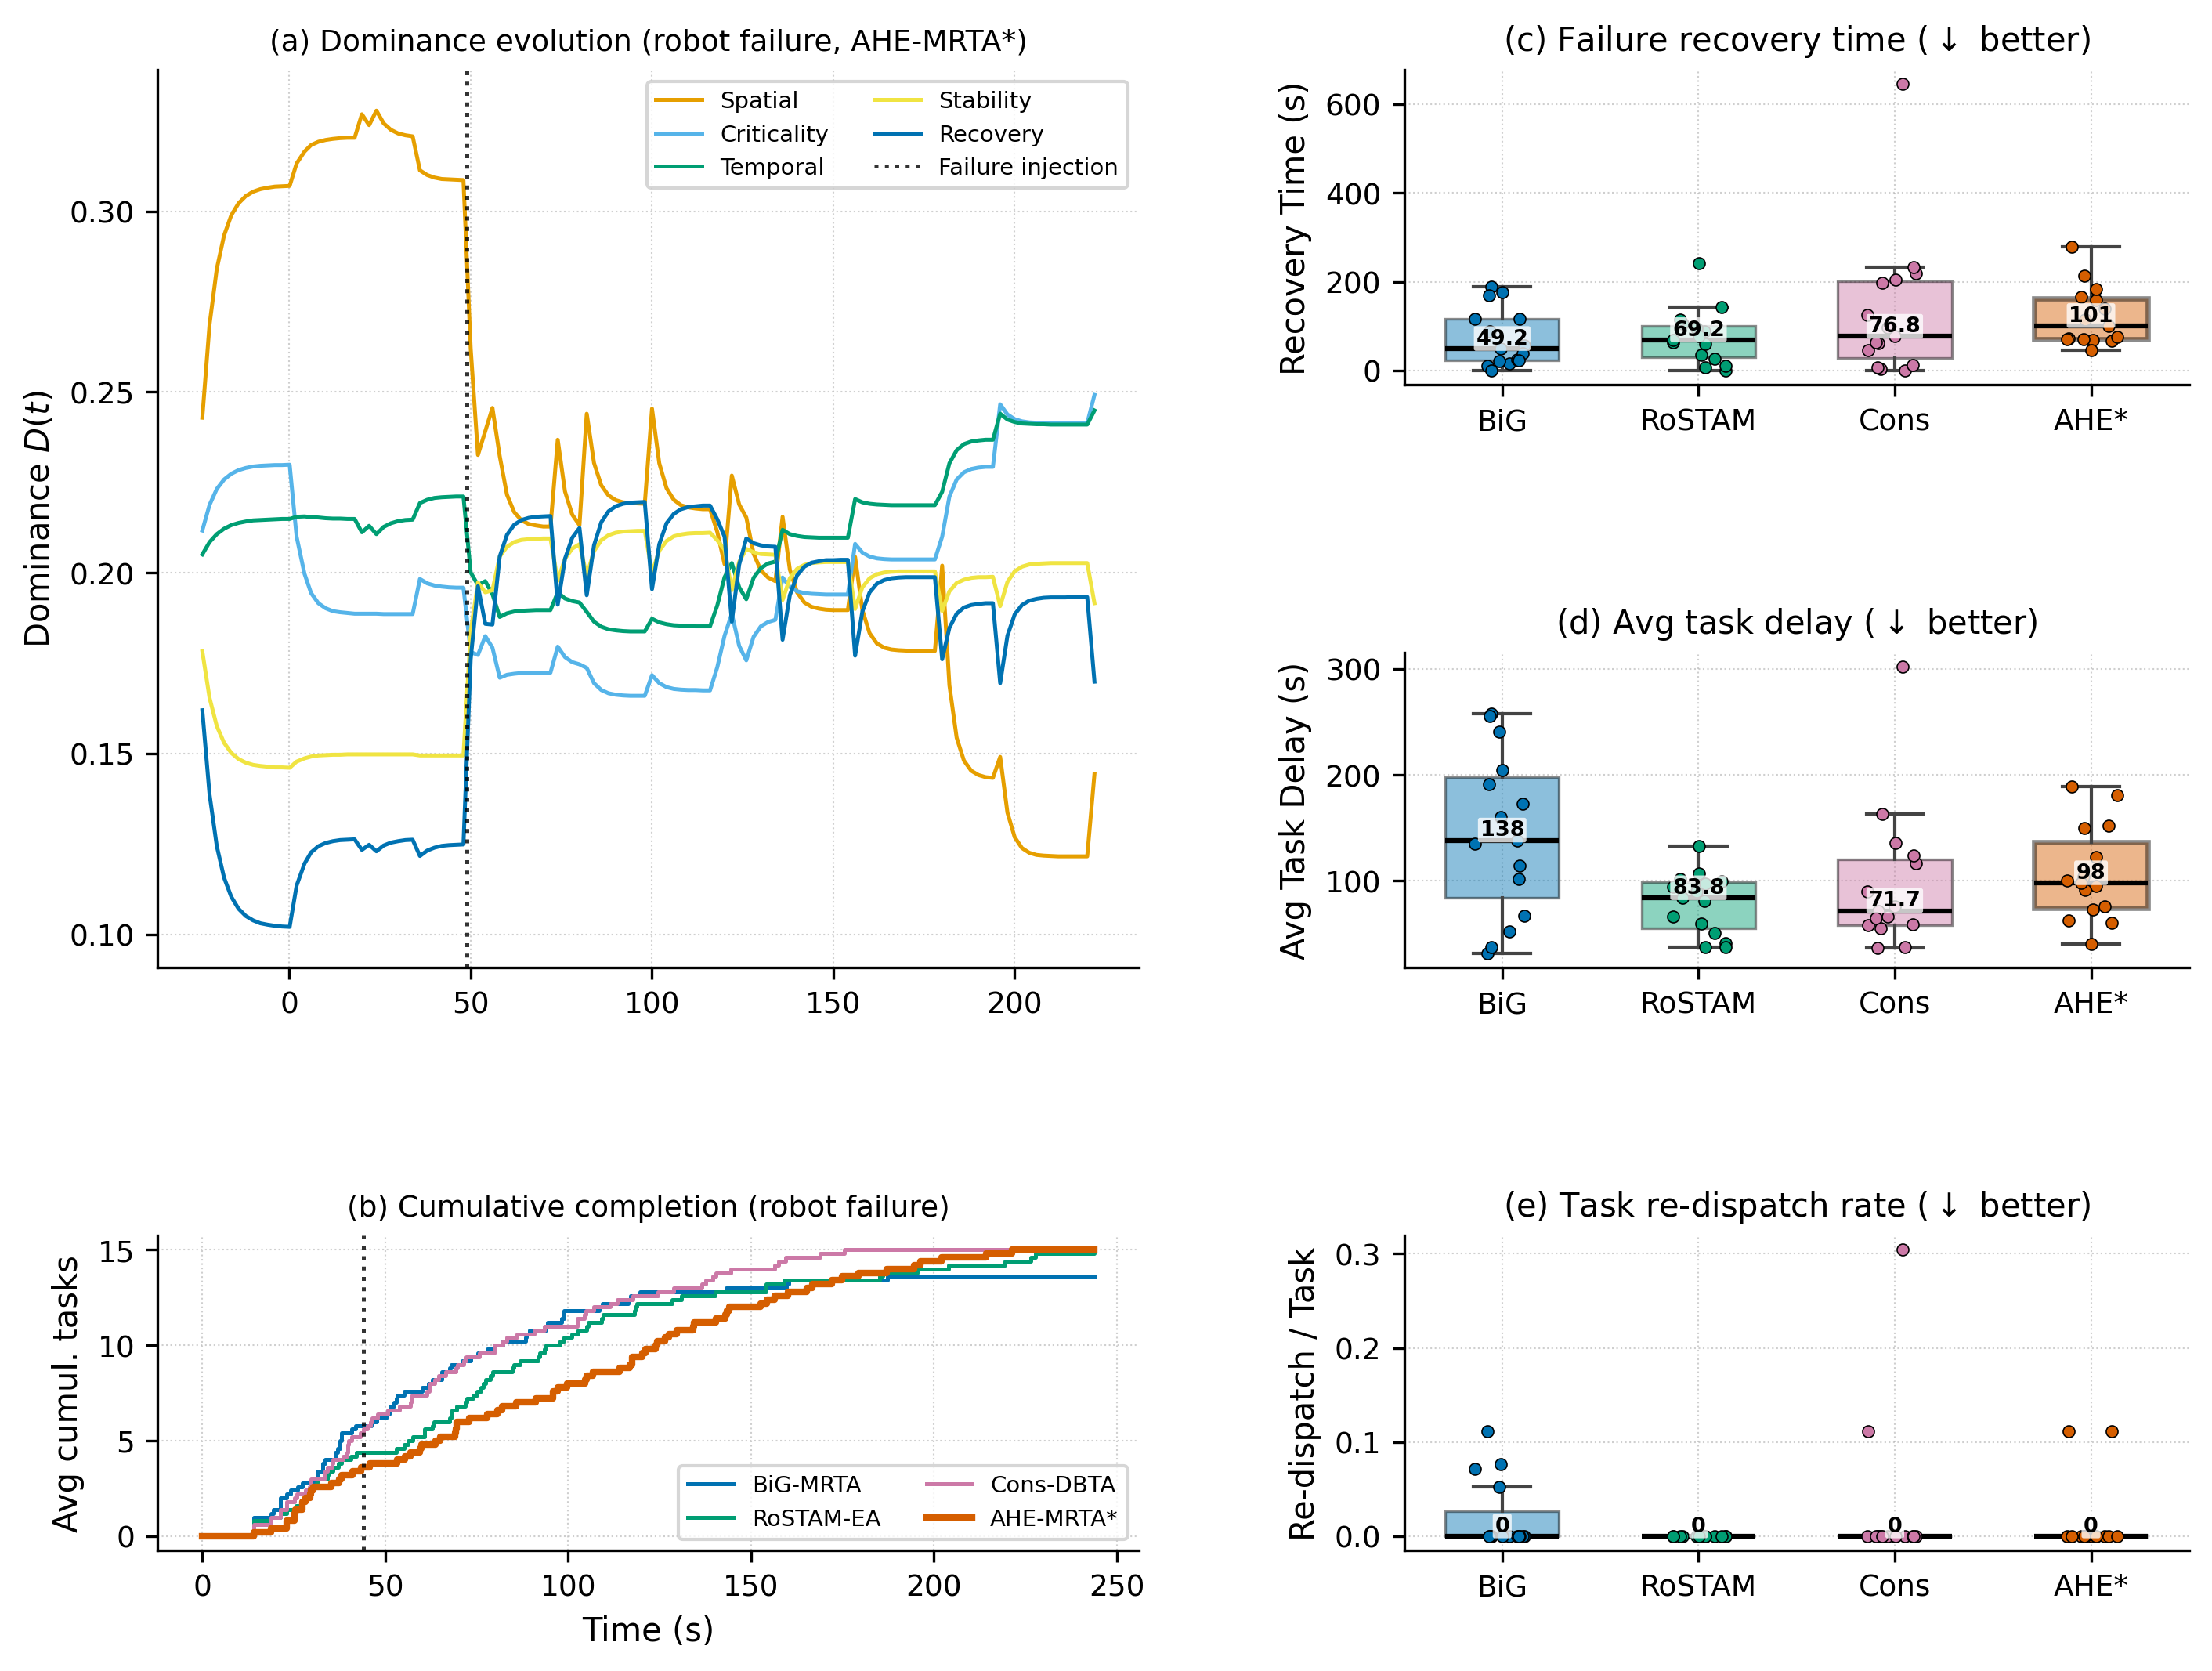
\includegraphics[width=\textwidth]{dominance_recovery_panel.png}
  \caption{\textit{robot\_failure} altında 3-robot ölçeğindeki uyum davranışı.
  (a)--(b) panelleri 15 görevli koşulları, (c)--(d) panelleri üç yoğunluğun
  birleştirilmiş sonuçlarını kullanır. Zaman her koşuldaki ilk görev
  etkinleşmesinden itibaren ölçülmüştür. Bu nedenle (a) ve (b)'deki arıza
  işaretleri senaryonun $45\pm5$~s zamanlamasıyla uyumludur.
  \textbf{(a)}~Temsilî bir AHE-MRTA koşusundaki hormon baskınlığı. Arıza
  öncesi evrede uzamsal hormon en yüksek değere sahiptir ($D{\approx}0.31$).
  Arıza enjeksiyonunda (noktalı çizgi, $t{\approx}49$~s) bu değer azalırken
  toparlanma ve kararlılık hormonları yükselir ($0.12{\to}0.20$ ve
  $0.15{\to}0.20$). Sonrasında hiçbir hormon arıza öncesi farkı geri
  kazanmaz. Uzamsal kanal yaklaşık bir dakika boyunca daha düşük bir farkla
  en yüksek değeri korur. Ardından zamansal ve kritiklik kanalları öne geçer
  ve gönderilen paradigma zamansal, uzamsal ve toparlanma politikaları
  arasında değişir.
  \textbf{(b)}~Tohum ortalamalı kümülatif görev tamamlama. Noktalı çizgi
  medyan arıza zamanını gösterir ($t{\approx}44$~s). AHE-MRTA arızadan sonra
  görevleri tamamlamayı sürdürür ve bütün görev kümesine ulaşır, ancak üç
  reaktif yöntem arasında bunu en geç tamamlayan yöntemdir.
  \textbf{(c--d)}~Toparlanma süresi ve ortalama görev gecikmesi kutu
  grafikleri. Kutu IQR'yi, çizgi medyanı, bıyıklar $1{,}5{\times}$IQR'yi ve
  noktalar tekil koşuları gösterir ($n{=}15$). AHE-MRTA'nın toparlanma süresi
  medyanı 101~s, diğer yöntemlerin medyanları 49--77~s'dir. AHE-MRTA'nın
  98~s'lik gecikme medyanı, uzlaşma yöntemlerinin 72--84~s değerleri ile
  görev terk eden BiG-MRTA'nın 138~s değeri arasındadır.}
  \label{fig:dom-recovery}
\end{figure}

\begin{figure}[t]
  \centering
  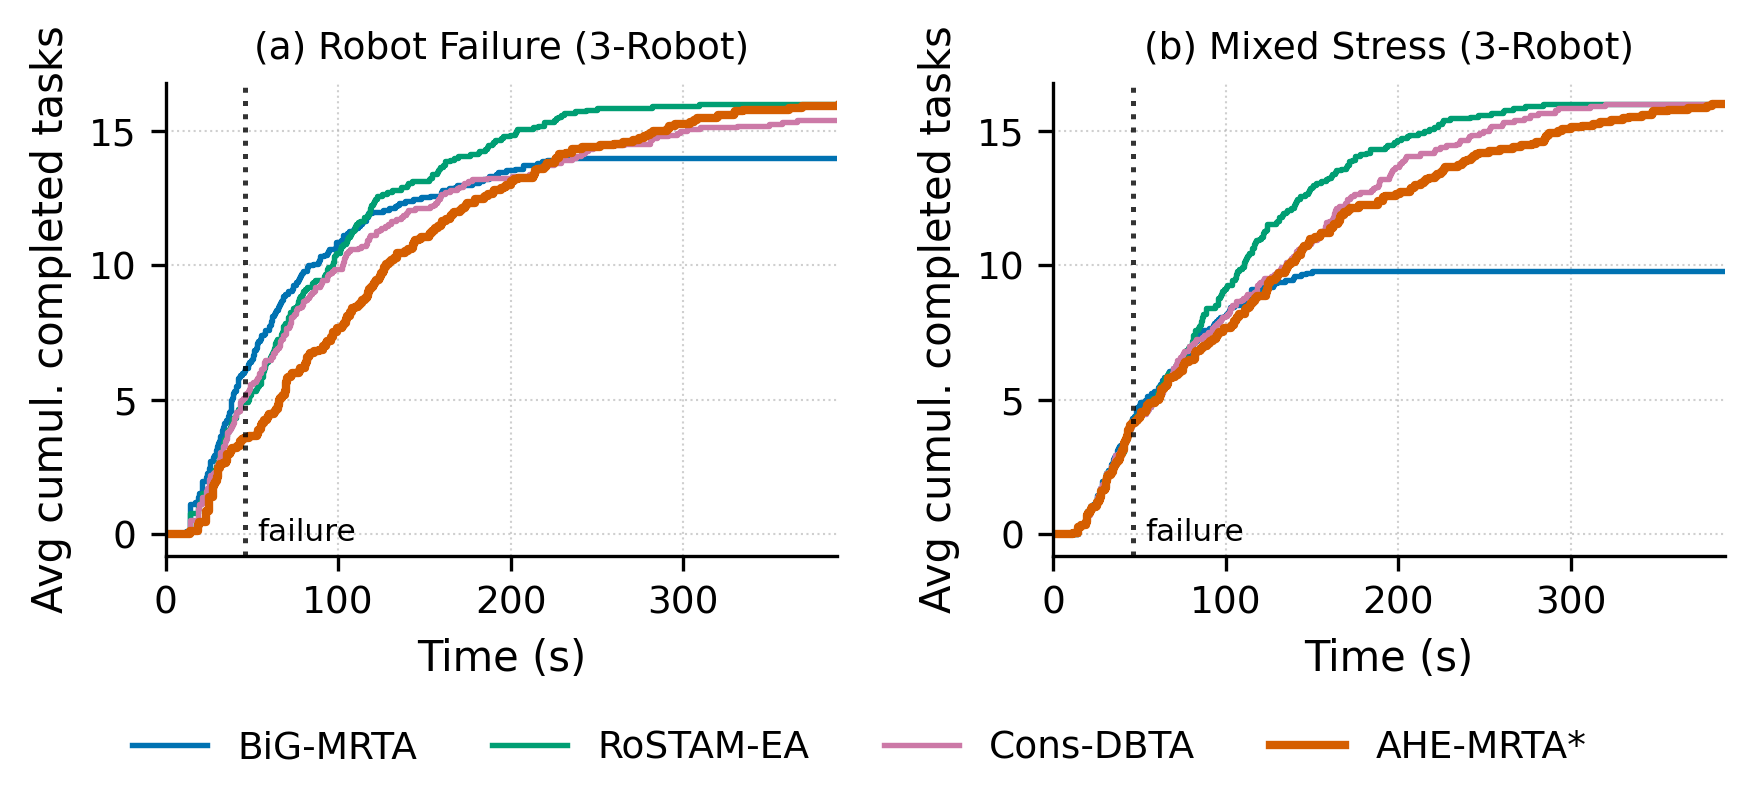
\includegraphics[width=0.85\textwidth]{task_completion_timeline.png}
  \caption{3-robot ölçeğinde zaman içinde kümülatif görev tamamlama,
  üç görev yoğunluğu üzerinden tohum-ortalamalı:
  \textbf{(a)}~\textit{robot\_failure}, \textbf{(b)}~\textit{mixed\_stress}.
  AHE-MRTA her iki senaryoda tam görev kümesini tamamlar. Toplam görev süresi
  \textit{robot\_failure}'da reaktif temel yöntemlerle aynı düzeydedir
  (AHE-MRTA 220~s, Cons-DBTA 224~s). \textit{mixed\_stress}'te ise yeniden
  atamayla ilişkili daha yüksek bir değere ulaşır (AHE-MRTA 243~s,
  Cons-DBTA 219~s,
  RoSTAM-EA 182~s).
  BiG-MRTA uygulanamaz olarak işaretlediği görevleri terk eder ve bütün görev
  kümesini tamamlamaz
  (Bölüm~\ref{sec:discussion}).}
  \label{fig:timeline}
\end{figure}

Navigasyondan bağımsız ve kapalı çevrim sonuçları arasındaki fark, iki deney
düzeyinin farklı etkileri içermesinden kaynaklanır. Hücre başına 100 tohumlu
belirlenimci yalnız-tahsis benzetimi, yerel planlayıcı duraklamaları, maliyet
haritası yeniden oluşturma işlemleri ve dar koridor manevraları gibi Nav2
kaynaklı değişkenliği içermez. Kabul edilen her rota ortak geodezik yürütme
modeliyle gerçekleştirilir. Gazebo'da ise iki ek etki bulunmaktadır:

\begin{enumerate}
  \item \textbf{Geçişler yürütme maliyeti oluşturur.} Bir paradigma değişimi,
    daha önce yönlendirilmiş bir görevin başka robota atanmasına neden olabilir.
    Bu durumda mevcut yol iptal edilir, Nav2 yeni bir plan üretir ve robot ek
    mesafe kat eder. Tek-atamalı temel yöntemler bu yeniden planlama maliyetini
    oluşturmaz.
  \item \textbf{Görev süresi fiziksel yürütmeden etkilenir.} Nav2 yürütmesi
    sırasında dünya geometrisi ve yerel hareket planı, görevin toplam süreye
    katkısını belirler. Ek yeniden planlama, en uzun yolun süresini artırabilir.
\end{enumerate}

Gazebo sonuçları bu etkilerle uyumludur. AHE-MRTA her hücrede tamamlama oranı
bakımından en yüksek veya eşit en yüksek değeri alır ve en güçlü temel yönteme
göre DVR'yi 5 robotta \%17, 10 robotta \%49 azaltır. Buna karşılık, 3 robotta
toplam yol 44--104~m yerine 99--113~m'dir. Karışık stres altındaki toplam görev
süresi, diğer iki reaktif yöntemde 182--219~s iken AHE-MRTA'da 243~s'dir.
Tek-atamalı BiG-MRTA bu hücrede 900~s deney ufkuna kadar çalışır. Beş robotta
uygulanan yeniden atama sayısı görev başına 0.014'ün altında kalır. On robotta
bu değer 0.06--0.08'e yükselir. Consensus-DBTA için 0.04--0.13, tek-atamalı
BiG-MRTA için 0.005--0.03'tür.

Aşağıdaki hücre düzeyindeki sonuçlar, değerlendirilen tam yapılandırmayı
betimler. Dört yöntemli karşılaştırmada birden çok bileşen aynı anda değiştiği
için bu sonuçlar paradigma değişiminin nedensel etkisini göstermez. Seçicinin
etkisi Bölüm~\ref{sec:gazebo-ablation}'daki eşleşmiş ablasyonla sınanmıştır.

\begin{itemize}
  \item \textbf{Son teslim uyumu.}
    \textit{deadline\_pressure}'da konsensüs ve evrimsel temel yöntemler,
    AHE-MRTA'ya benzer tamamlama oranlarına ulaşır. Ancak bu yöntemlerin son
    teslim ihlal oranları $1.2$--$2.3\times$ daha yüksektir. Beş robotta DVR,
    AHE-MRTA için 0.350, Consensus-DBTA için 0.422 ve RoSTAM-EA için 0.498'dir.
    On robotta karşılık gelen değerler 0.220, 0.428 ve 0.504'tür. AHE-MRTA'nın
    zamanında etkin tamamlaması iki ölçekte de en yüksektir (5r'de $0.650$,
    10r'de $0.764$). Dört yöntemli karşılaştırma bu işletim örüntüsünü
    destekler, ancak seçiciye özgü açıklamayı desteklemez.
  \item \textbf{Arıza sonrası toparlanma.}
    \textit{robot\_failure} altında AHE-MRTA, 5 robotta tam tamamlamayı
    (CR\,=\,1.000, DVR\,=\,0.014, zamanında etkin tamamlamada $0.986$ ve
    temel yöntemlerde ${\leq}0.890$) ve 10 robotta eşit en yüksek tamamlamayı
    (CR\,=\,0.976, zamanında etkin tamamlamada BiG-MRTA ile aynı
    seviyede) birlikte sağlar. Yöntem arıza sonrası sahipsiz görevleri yeniden
    atar. Mevcut dört yöntemli karşılaştırma bu davranışın marjinal nedensel
    etkisini tanımlamaz.
  \item \textbf{Küçük ölçekte tamamlama oranı.} Üç robotta tekdüze son teslim
    baskısı
    altında EDF temelli yöntemler Gazebo'da tam tamamlamaya ulaşır.
    RoSTAM-EA, Cons-DBTA ve AHE-MRTA için CR\,=\,1.000'dır. Yalnızca görevleri
    terk eden BiG-MRTA, 0.633'te kalır. Dolayısıyla bu ölçekte tamamlama oranı
    yöntemleri ayırmaz. Kalan fark son teslim uyumundadır
    (zamanında etkin tamamlama: AHE-MRTA 0.69, temel yöntemler 0.60--0.66).
    Bu farkla birlikte toplam görev süresi 146--159~s yerine 179~s, gecikme
    70--77~s yerine 80~s ve yol uzunluğu 77--86~m yerine 99~m olur. Aynı
    ölçekte navigasyon vekilinde zamanında uygunluk AHE-MRTA için 0.420,
    BiG-MRTA için 0.417'dir
    (Tablo~\ref{tab:scalability}).
    Ancak 10 robotta AHE-MRTA, temel yöntemlerin 0.428--0.504 aralığına karşı
    DVR'ı
    0.220'de tutar ve en yüksek zamanında-etkin tamamlamaya ulaşır
    (Bölüm~\ref{sec:results-gazebo}).
\end{itemize}

\phantomsection
\label{sec:deadline-tie}
Stokastik navigasyon vekilinde AHE-MRTA her senaryoda en yüksek öncelik
ağırlıklı zamanında tamamlama değerine ulaşır. Bununla birlikte, en güçlü
temel yönteme göre fark $0.004$--$0.065$ aralığındadır ve bütün yöntemler
navigasyon arızası bulunmayan düzeyin altında kalır
(Tablo~\ref{tab:fitness}). Aynı politikalar navigasyon arızası bulunmadığında
$0.642$--$0.994$, bulunduğunda $0.217$--$0.384$ elde eder. Bu düşüşün temel
kaynağı konuma bağlı stokastik navigasyon arızaları ve yeniden denemelerdir.
AHE-MRTA ile Consensus-DBTA başarısız ve sahipsiz görevleri yeniden atayarak
bu etkiyi sınırlar. Robot arızası altında tek-atamalı BiG-MRTA da koşula uygun
bir davranış gösterir ve AHE-MRTA ile fark $0.004$'tür. Bu karşılaştırma
anlamlı değildir. En güçlü temel yönteme göre fark karışık streste $+0.034$,
son teslim baskısında $+0.065$'e çıkar.

Vekil ölçütü yalnız son teslim süresinden önce tamamlanan görevleri
puanlandırır. Geç tamamlanan ve tamamlanmayan görevlerin ikisi de sıfır puan
alır. AHE-MRTA süresi geçmiş görevleri yeniden atamayı sürdürdüğü için ham
tamamlama oranını artırabilir, ancak geç tamamlanan görevler zamanında
tamamlama puanı üretmez. Tek-atamalı yöntemler ise bazı görevleri terk eder ve
yalnız tamamladıkları görevler üzerinden değerlendirilir. Bu fark, AHE-MRTA'nın
kapalı çevrimde tam tamamlama ve sahipsiz görev bırakmama davranışıyla
uyumludur (Bölüm~\ref{sec:results-gazebo}). Son teslim fizibilitesini dikkate
alan ek yürütme sıralaması tek başına uygunluğu yaklaşık ${\approx}1.3$~yüzde
puan artırmıştır. Bağlam sinyalleriyle etkinleştirildiğinde ise aynı kural,
tamamlama hızının belirleyici olduğu karışık koşullarda uygunluğu benzer
ölçüde azaltmıştır. Bu nedenle raporlanan yapılandırmada bütünlük odaklı
politika korunmuştur.

\subsection{Ablasyon Analizi}
\label{sec:ablation}
Çevrim içi paradigma değişiminin katkısı, seçicinin ayrı ayrı her sabit
paradigmayla değiştirilmesiyle incelenmiştir. Ek olarak, diğer bileşenler sabit
tutularak bağlam geçersiz kılmaları (\emph{no-override}: yalnız
$\arg\max_i D_i$) ve toparlanma artışı
(\emph{no-recovery-boost}: $\delta{=}0$) devre dışı bırakılmıştır. Deney,
5r/25g ölçeğinde 100 tohum ve geodezik yürütme modeli kullanan stokastik
navigasyon vekilinde yürütülmüştür.

% GENERATED by scripts/make_proxy_tables.py -- do not edit by hand.
\begin{table}[t]
\centering
\caption{Seçici ablasyonu (stokastik navigasyon vekili, geodezik yürütme kâhini, 5r/25g, 100 tohum). Düzeltilmiş senaryo parametreleriyle varyantlar ortalama uygunlukta 0.101 aralığa yayılır. Bağlam geçersiz kılmalarını kaldırmak seçiciyi neredeyse hiç değiştirmez ve bu düzlemde sabit spatial-greedy onun önündedir; her iki gözlem de kapalı-çevrim ablasyonunda (Bölüm~\ref{sec:gazebo-ablation}) sınanır.}
\label{tab:ablation}
\small
\setlength{\tabcolsep}{4pt}
\begin{tabular}{lcccc}
\toprule
\textbf{Varyant} & \textbf{Arıza} & \textbf{Deadline} & \textbf{Karışık} & \textbf{Ortalama} \\
\midrule
\textbf{Full EDPS} & 0.383 & 0.348 & 0.255 & 0.329 \\
fixed: spatial & 0.421 & 0.358 & 0.265 & \textbf{0.348} \\
fixed: priority & 0.357 & 0.298 & 0.274 & 0.310 \\
fixed: edf & 0.333 & 0.296 & 0.276 & 0.302 \\
fixed: commit & 0.344 & 0.186 & 0.210 & 0.247 \\
fixed: orphan & 0.318 & 0.259 & 0.254 & 0.277 \\
no-override & 0.384 & 0.331 & 0.254 & 0.323 \\
no-recovery-boost & 0.382 & 0.348 & 0.255 & 0.328 \\
\midrule
\multicolumn{5}{l}{\footnotesize Tam seçici ortalaması 0.329; en iyi varyant 0.348.} \\
\bottomrule
\end{tabular}
\end{table}


Yapılandırmaların ortalama uygunlukları $0.101$ aralığına yayılmıştır. Bağlam
geçersiz kılmalarının kaldırılması uygunluğu $0.329$'dan $0.323$'e, toparlanma
artışının kaldırılması ise $0.328$'e değiştirmiştir. Sabit uzamsal açgözlü
paradigma $0.348$ ile tam seçicinin $0.329$ değerinin üzerindedir. Diğer dört
sabit paradigma tam seçiciden $0.02$--$0.08$ daha düşük uygunluk göstermiştir.
Bu bulgular, vekil düzeyinde geçersiz kılma katmanının sınırlı etkisini ve
seçicinin en sık kullandığı sabit davranışın rekabetçi olduğunu gösterir.

Vekil düzeyi tıkanıklığı, yeniden planlama gecikmesini ve toparlanma süresini
modellemediğinden bu sonuçlar doğrudan kapalı çevrime aktarılamaz. Eşleşmiş
kapalı çevrim ablasyonu, geçersiz kılmaların sınırlı etkisini doğrularken
önceden belirlenen iki sabit paradigmanın daha düşük başarım verdiğini
göstermiştir. Sabit uzamsal açgözlü yapılandırma önceden belirlenen tasarımın
parçası değildir ve Bölüm~\ref{sec:gazebo-ablation}'da keşifsel bir
karşılaştırma olarak raporlanmaktadır.

Geodezik seyahat kestiriminin etkisi ikinci bir eşli A/B deneyiyle ayrı olarak
incelenmiştir. Beş yüz ortak tohum boyunca tahsis maliyeti geodezik ETA ile
Öklid uzaklığı arasında değiştirilmiş, yürütme modeli her iki durumda da
geodezik tutulmuştur. Böylece iki yapılandırma aynı zemin gerçeği üzerinde
değerlendirilmiştir. Temel yöntemler bu yapılandırma bayrağını kullanmadığı için
iki koşulda aynı sonuçları üretmiştir. Geodezik yapılandırma,
Tablo~\ref{tab:fitness}'teki kampanya sonuçlarını dokuz ondalık basamağa kadar
yeniden üretmiştir. Geodezik ETA robot arızasında $+2.13$~yüzde puan, karışık
streste $+1.83$~yüzde puan ve son teslim baskısında $+4.10$~yüzde puan katkı
sağlamıştır. Beş yüz eşleşmiş örnekte üç karşılaştırma için de $p<10^{-4}$'tür.
Cliff $\delta$ değerleri robot arızası ve karışık stres için sırasıyla $0.131$
ve $0.128$, son teslim baskısı için $0.275$'tir. Etki ilk iki senaryoda ihmal
edilebilir, son senaryoda küçüktür. Dolayısıyla geodezik ETA tutarlı fakat
sınırlı bir katkı sağlamaktadır ve ana başarım farkını tek başına açıklamaz.

Eşleşmiş kapalı çevrim ablasyonunda seçici dışındaki bütün bileşenler sabit
tutulmuştur.
\phantomsection
\label{sec:gazebo-ablation}
Önceden belirlenen dört yapılandırma \emph{full}, \emph{no-override} (yalnız
$\arg\max_i D_i$) ve seçicinin kullandığı iki sabit paradigmadan oluşur.
Deney, 5 robot/25 görev ölçeğinde üç senaryo ve 20 ortak tohumla toplam 240
koşu içerir. Hipotezler, yapılandırmalar, uç noktalar, istatistik planı ve
analiz yazılımı kampanya tamamlanmadan önce sabitlenmiş ve deney yapıtlarıyla
birlikte arşivlenmiştir. Kayıp tohum bulunmadığından 20 tohumun tamamı bütün
yapılandırmalarda eşleşmektedir.

% ÜRETİLEN dosya: scripts/analyze_ablation.py -- elle düzenleme.
% results/raw/gazebo_ablation/ değişince yeniden üret.
\begin{table}[t]
\centering
\caption{Birincil 5-robot/25-görev ölçeğindeki eşleşmiş kapalı çevrim
ablasyonu. Dört yapılandırma, senaryo başına 20 ortak tohumla değerlendirilmiş
ve deney tasarımı kampanya öncesinde kayıt altına alınmıştır. Birincil uç nokta,
\textit{deadline\_pressure} senaryosundaki zamanında etkin tamamlamadır
$\mathrm{CR}\times(1-\mathrm{DVR})$. $p$ değerleri, \emph{full}
yapılandırmasına karşı eşli Wilcoxon işaretli sıra testinden elde edilmiş ve
senaryo ailesi içinde Bonferroni yöntemiyle düzeltilmiştir. Cliff $\delta$ için
önyükleme tabanlı \%95 güven aralığı kullanılmıştır. Diğer iki senaryo
betimleyici olarak raporlanmıştır. Sütunlar sırasıyla \emph{full},
\emph{no-override}, \emph{fixed-EDF} ve \emph{fixed-orphan} uygulama
yapılandırmalarına karşılık gelir.}
\label{tab:gazebo-ablation}
\small
\setlength{\tabcolsep}{4pt}
\begin{tabular}{l cccc}
\toprule
& \textbf{Tam} & \textbf{Zincirsiz} & \textbf{Sabit EDF} & \textbf{Sabit sahipsiz} \\
\midrule

\multicolumn{5}{l}{\textit{deadline\_pressure} -- birincil uç nokta} \\
\quad zamanında-etkin tamamlama & 0.650 & 0.641 & 0.556 & 0.540 \\
\quad $p$ (Bonferroni) & -- & 1.000 & $<$0.005 & $<$0.005 \\
\quad Cliff $\delta$ (full'e karşı) & -- & +0.06 & +0.57 & +0.62 \\
\midrule
\multicolumn{5}{l}{\textit{robot\_failure} -- betimleyici} \\
\quad zamanında-etkin tamamlama & 0.986 & 0.998 & 0.846 & 0.850 \\
\quad tamamlama oranı & 1.000 & 1.000 & 0.998 & 1.000 \\
\quad toparlanma süresi (s) & 83.7 & 63.3 & 88.5 & 56.6 \\
\midrule
\multicolumn{5}{l}{\textit{mixed\_stress} -- betimleyici} \\
\quad zamanında-etkin tamamlama & 0.616 & 0.606 & 0.590 & 0.601 \\
\bottomrule
\end{tabular}
\end{table}


Tablo~\ref{tab:gazebo-ablation}, sabit paradigma kullanmanın ve belirli geçiş
mekanizmasının etkilerini ayrı karşılaştırmalarla göstermektedir. Tahsis
edicinin iki sabit paradigmadan birine sınırlandırılması, son teslim baskısı
altında zamanında etkin tamamlamayı $0.650$'den $0.556$ ve $0.540$'a düşürür.
Fark $9$--$11$ yüzde puanıdır. Etki büyüklükleri $\delta=0.57$ ve $0.62$ olup
Bonferroni düzeltmesinden sonra anlamlıdır ($p<0.005$). Robot arızasında
paradigma değiştiren yapılandırmalar yaklaşık $0.99$, sabit yapılandırmalar
yaklaşık $0.85$ elde eder. Navigasyon vekilinde de aynı iki sabit paradigma,
tam seçicinin $0.348$ değerine karşı $0.296$ ve $0.259$ elde eder
(Tablo~\ref{tab:ablation}). Sabit EDF için fark vekilde $5.2$, kapalı çevrimde
$9.4$ yüzde puanıdır. Nedensel çıkarım, ortak tohumlarla yürütülen ve çoklu
karşılaştırma için düzeltilen kapalı çevrim deneyiyle sınırlıdır.

Bağlama bağlı öncelikli seçim zincirinin kaldırılması birincil uç noktayı
$0.650$'den
$0.641$'e değiştirmiştir. Fark anlamlı değildir
($p_{\mathrm{adj}}=1.000$, $\delta=0.06$). Robot arızasında
\emph{no-override} yapılandırması $0.998$, tam yapılandırma $0.986$ elde
etmiştir. Toparlanma süreleri sırasıyla 63~s ve 84~s'dir. Bu farkların ikisi de
çoklu karşılaştırma düzeltmesinden sonra anlamlı değildir. Sonuç, bu
senaryolarda öncelikli seçim zinciri ile baskınlık tabanlı seçimin benzer
politikalara erişebildiğini, uygulanan zincirin ayrıca ölçülebilir bir katkı
sağlamadığını göstermektedir.

Önceden belirlenen iki sabit yapılandırma, geçersiz kılma kurallarının hedef
politikalarıdır. Buna karşılık baskınlık katmanı karar verdiği durumların
\%$99.9$'unda uzamsal açgözlü politikayı seçmektedir
(Bölüm~\ref{sec:limitations}). Vekil ablasyonunda bu sabit politika tam
seçiciden daha yüksek uygunluk sağlamıştır (Tablo~\ref{tab:ablation}). Bu
nedenle uzamsal açgözlü politika, aynı 20 tohumda eşleşmiş beşinci bir
yapılandırma olarak sonradan eklenmiştir. Bu karşılaştırma keşifseldir ve
birincil Bonferroni ailesine dahil değildir. Birincil uç noktada tam seçici
$0.650$, sabit uzamsal açgözlü $0.638$ elde etmiştir. Fark anlamlı değildir
($p=0.43$, $\delta=+0.09$). Sabit politika robot arızasında $0.998$ ile tam
seçicinin $0.986$ değerinin üzerinde (ham $p=0.014$, $\delta=-0.30$), karışık
streste ise $0.584$ ile $0.616$ değerinin altındadır (ham $p=0.038$). Bu iki
karşılaştırma, önceden belirlenen dört yapılandırmaya uygulanan düzeltme
eşiğini geçmezdi.

Bu sonuçlar iddiayı iki yönden sınırlar. Sabit EDF ve sabit sahipsiz-görev-önce
politikaları zamanında etkin tamamlamada $9$--$11$ yüzde puan kaybettirir.
Buna karşılık tam seçici, öncelikli seçim zinciri olmadan çalışan seçici ve
sabit uzamsal açgözlü politika sırasıyla $0.650$, $0.641$ ve $0.638$ ile benzer
başarım gösterir. Dolayısıyla
kanıt, portföyün koşula uygun bir politika içermesi ve tahsis edicinin uygun
olmayan bir politikaya sabitlenmemesi gerektiğini destekler. Uygulanan
seçicinin uzamsal açgözlü politikaya üstün olduğunu göstermez. Bu ayrımın
değerlendirilmesi, uzamsal açgözlü politikanın yetersiz kaldığı ve seçicinin
başka bir politikaya geçmesini gerektiren deney koşulları gerektirir. Mevcut
karışık stres sonucu bu gereksinimi tek başına karşılamaz.

Eşleşmiş ablasyonun iki ek sınırı vardır. Robot arızası için önceden belirlenen
ikincil uç nokta olan tamamlama oranı dört yapılandırmada da $\geq0.998$'dir ve
yapılandırmaları ayırmaz. Bu senaryodaki zamanında etkin tamamlama sonuçları,
yalnızca birincil senaryo için önceden tanımlandığından betimleyici olarak
raporlanmıştır. Ayrıca bütün kapalı çevrim ablasyonları tek bir arenada
yürütülmüştür. Deney seçici dışındaki bileşenleri denetim altında tutar, ancak
ortamlar arası genellenebilirliği göstermez.

Ablasyonlarla birlikte hesaplama ve haberleşme maliyetleri de incelenmiştir.
AHE-MRTA yalnızca robot başına optimize edilmiş görev kuyruklarını yayınlar.
Baskınlık vektörü, işbirliği ve baskılama matrisleri ile küresel maliyet matrisi
merkezi yöneticide kalır. Haberleşme yükü, her olayda iletilen alanların sayısı
ve boyutu üzerinden aynı yöntemle hesaplanmıştır. Bir kuyruk girdisi 4~baytlık
görev kimliği, her robot başlığı 8~bayt, bir teklif kaydı 16~bayt ve bir fayda
matrisi girdisi 4~bayttır. Şekil~\ref{fig:comm}, olay başına haberleşme yükünü
göstermektedir. Ölçekler birleştirildiğinde ortalama yük AHE-MRTA için 63~bayt,
tek-atamalı temel yöntemler için 134 ve 239~bayt, RoSTAM-EA için
$1{,}7{\times}10^{4}$~bayttır. Yöntemlerin ölçeklenme biçimleri farklı olduğu
için birleştirilmiş değerler tek başına yeterli değildir. AHE-MRTA'nın yükü 3,
5 ve 10 robotta sırasıyla 40, 71 ve 137~bayttır. Aynı aralıkta BiG-MRTA
71\,$\to$\,697, Consensus-DBTA 89\,$\to$\,684 ve RoSTAM-EA
$7{,}4{\times}10^{3}$\,$\to$\,$2{,}6{\times}10^{4}$~bayta yükselir. Bu deney
yalnızca mesaj yükünü ölçmektedir. Geçiş sıklığı değiştirilmediğinden, bu
sıklığa bağlı davranış hakkında nedensel bir sonuç desteklemez.

\begin{figure}[t]
  \centering
  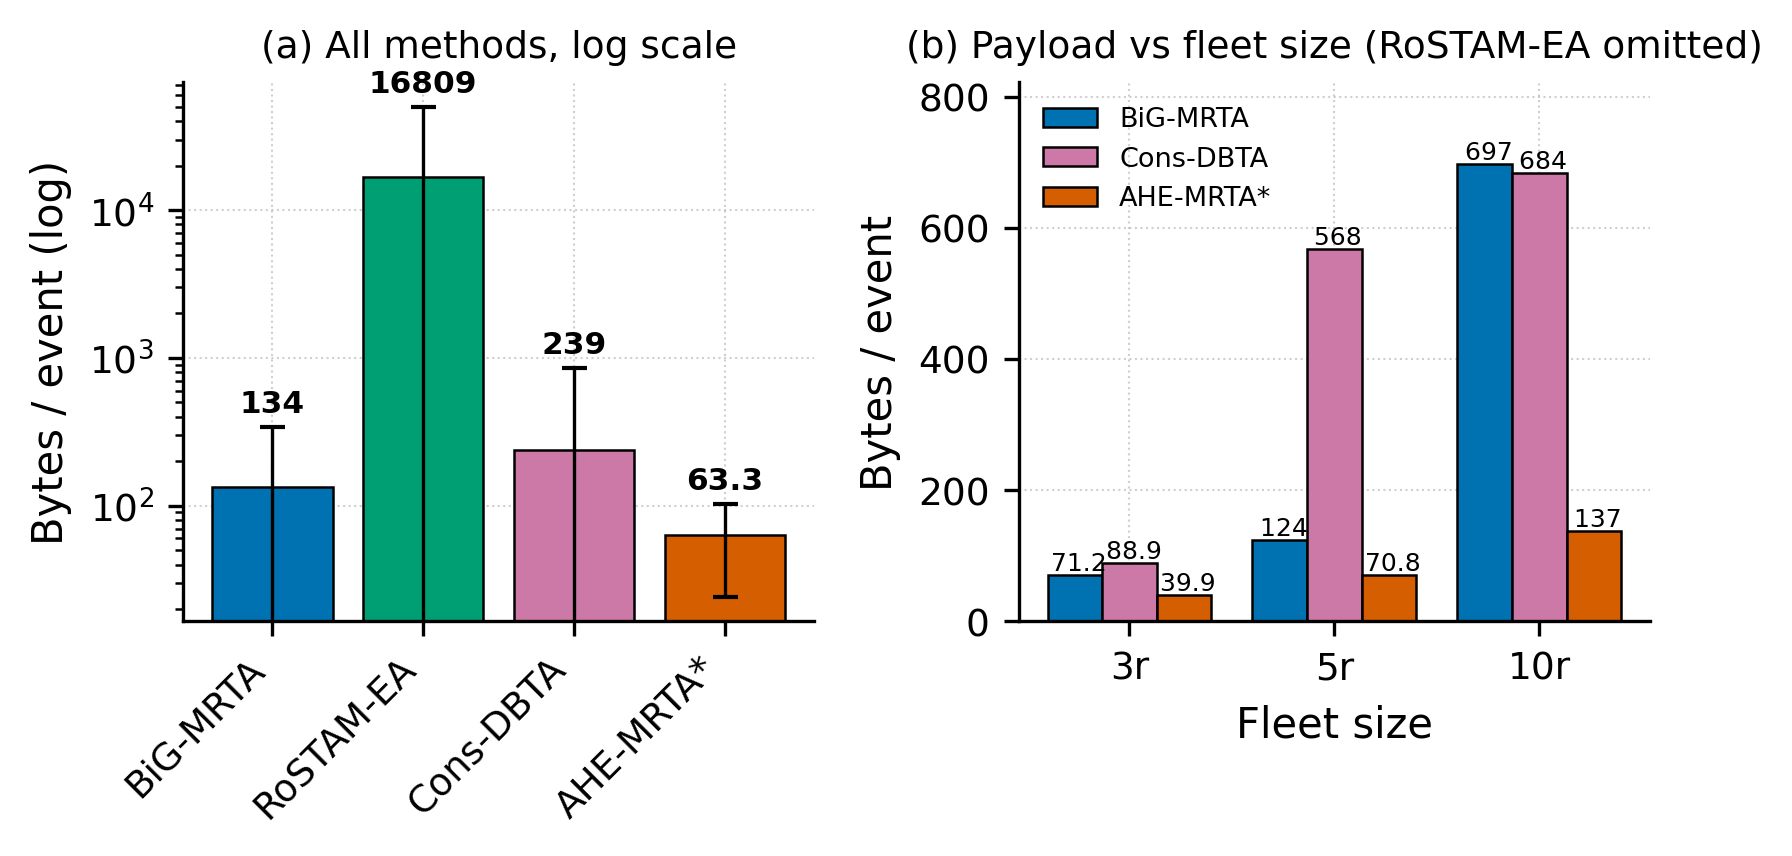
\includegraphics[width=0.80\textwidth]{communication_footprint.png}
  \caption{Tahsis olayı başına haberleşme yükü, her protokolde iletilen alanlar
  üzerinden hesaplanmıştır. \textbf{(a)}~Ölçekler birleştirilerek bütün
  yöntemlerin karşılaştırılması (logaritmik eksen). \textbf{(b)}~RoSTAM-EA
  dışındaki yöntemler için filo büyüklüğüne göre yük. AHE-MRTA yalnız robot
  başına kuyruk yayımladığı için yükü robot sayısıyla doğrusal artar. Teklif ve
  fayda matrisi alışverişleri ise robot ve görev sayılarının çarpımıyla artar.}
  \label{fig:comm}
\end{figure}

%==============================================================================
\section{Tartışma}
\label{sec:discussion}

\subsection{Temel Bulguların Yorumu}

Üç değerlendirme düzeyi birlikte değerlendirildiğinde, arıza ve son teslim
baskısı altında koşula uygun bir tahsis politikasına erişimin önemli olduğu
görülmektedir. Bununla birlikte eşleşmiş ablasyonlar, uygulanan çevrim içi
geçiş kuralının en güçlü sabit politikaya göre ayrıca ölçülebilir bir üstünlük
sağladığını göstermemektedir. Bulgular bu nedenle politika portföyünün
uygunluğunu destekler, belirli seçicinin genel olarak üstün olduğu sonucunu
desteklemez.

Deney düzeyleri farklı araştırma sorularını yanıtlamaktadır. Navigasyondan
bağımsız benzetim tahsis ve kuyruk sıralamasını, stokastik vekil navigasyon
arızasına karşı dayanıklılığı, Gazebo ise tahsis, hareket planlama, sıkışıklık
ve yeniden planlamanın birlikte etkisini ölçer. Kapalı çevrimde bu yürütme
etkileri yöntemler arasındaki farkın büyüklüğünü ve yönünü değiştirebilir.
Dolayısıyla benzetim sonuçları kapalı çevrim başarımının doğrudan kestirimi
olarak yorumlanmamalıdır.

AHE-MRTA son teslim uyumu ve görev tamamlama bakımından avantaj sağlarken daha
uzun yollar, bazı koşullarda daha yüksek görev gecikmesi ve tek-atamalı
yöntemlerden daha yüksek karar gecikmesi oluşturur. Bununla birlikte karar
süreleri belirlenen gerçek zaman bütçesi içinde kalmaktadır. Uygulama açısından
temel tercih, son teslim uyumu ve arıza sonrası görev bütünlüğü ile yol,
gecikme ve iş yükü dengesi arasındaki ödünleşime bağlıdır.

\subsection{Sınırlılıklar}
\label{sec:limitations}

Sınırlılıklar kanıtın gücü, deney kapsamı ve uygulanan model bakımından aşağıda
özetlenmiştir.

\begin{enumerate}
  \item \textbf{İstatistiksel güç filo ölçeğine göre değişmektedir.}
  Birincil 5-robot ölçeğinde hücre başına örneklem büyüklüğü $n{=}20$'dir ve
  düzeltilmiş çıkarımı desteklemektedir. Aynı hücrelerde $n{=}5$ kullanıldığında
  63 karşılaştırmanın hiçbiri düzeltme eşiğini geçmezken, $n{=}20$ ile 20
  karşılaştırma eşiği geçmiştir. Tohum sayısı artırıldığında dört yöntemin
  zamanında etkin tamamlama nokta tahminleri $0.08$--$0.16$ azalmış, yöntem
  sıralaması ise korunmuştur. Üç robotlu hücreler $n{=}15$, 10 robotlu hücreler
  $n{=}5$ içerir. Bu nedenle 10-robot sonuçları betimleyicidir. Beş yüz tohumlu
  vekil deneyleri yalnızca vekil düzeyinde yüksek güçlü karşılaştırmaları
  destekler.

  \item \textbf{Baskınlık dinamiğinin değerlendirilen senaryolardaki rolü
  sınırlıdır.} Robot arızası ve son teslim baskısı çoğunlukla belirlenimci
  bağlam geçersiz kılmalarıyla ele alınır (Bölüm~\ref{sec:method}). Yüz yirmi
  AHE-MRTA koşusunda kaydedilen $15{,}058$ durumun yeniden değerlendirilmesinde
  seçimlerin \%$49{,}2$'si arıza, \%$25{,}3$'ü son teslim geçersiz kılması ve
  \%$25{,}5$'i baskınlık katmanı tarafından belirlenmiştir. Baskınlık katmanı
  kendi kararlarının \%$99{,}9$'unda uzamsal açgözlü politikayı seçmiştir. Bu
  katmanın sabit bir seçimle değiştirilmesi, $15{,}058$ durumun yalnız 3'ünde
  (\%$0{,}02$) seçimi değiştirir. Tek-atamalı politika hiçbir durumda,
  öncelik-önce politikası ise yalnız bir durumda seçilmiştir. Dolayısıyla
  yöntem, yalnız dinamik bir seçici olarak değil, dinamik bir geri dönüş
  katmanı içeren bağlam güdümlü bir seçim yapısı olarak yorumlanmalıdır.
  Tablo~\ref{tab:ablation}'de bağlam geçersiz kılmalarını kaldırmak vekil
  uygunluğunu $0{,}6$ yüzde puan, toparlanma artışını kaldırmak $0{,}1$ yüzde
  puan azaltır. Sabit politikalar ise seçicinin $1{,}9$ yüzde puan üstünden
  $8{,}2$ yüzde puan altına kadar değişir (Bölüm~\ref{sec:ablation}).

  \item \textbf{Kapalı çevrim ablasyonu portföy ve geçiş mekanizması için
  farklı sonuçlar vermektedir.} Bölüm~\ref{sec:gazebo-ablation}'daki deney,
  seçici dışındaki bütün bileşenleri 20 ortak tohum boyunca sabit tutar. Sabit
  ve uygun olmayan bir politikaya sınırlandırma büyük ve düzeltilmiş bir fark
  oluştururken, uygulanan seçici daha basit $\arg\max_i D_i$ kuralından ayırt
  edilememiştir. Bu nedenle kanıt, uygun bir portföy üzerinde çevrim içi politika
  seçimini destekler. Bağlama bağlı öncelikli seçim zincirinin üstün bir geçiş
  kuralı olduğunu
  göstermez. Geçiş kuralları arasında genel bir sıralama için daha geniş bir
  kural taraması gereklidir. Deneyin tek arenayla sınırlı olması da ortamlar
  arası genellemeyi engeller.

  \item \textbf{Yöntemler eşit düzeyde ayarlanmamıştır.} AHE-MRTA raporlanan
  arena ve üç senaryoya göre geliştirilmiş ve sabitleri bu koşullarda
  belirlenmiştir. Temel yöntemler kaynak tanımlarından uygulanmış, ancak aynı
  kapsamda yeniden ayarlanmamıştır. Ayrıca onarım toleransı ve rezervasyon
  aralığı için kullanılan 401--420 tohumları, Bölüm~\ref{sec:results-sim}'deki
  1--500 raporlama aralığının içindedir. Dolayısıyla karşılaştırma, soyut
  algoritmaların eşit ayarlanmış sürümlerinden çok, ortak yürütme yığınındaki
  yapılandırılmış yöntemler için kanıt sağlar.

  \item \textbf{Kapalı çevrim ölçeği ana makine kaynaklarıyla sınırlıdır.}
  On beş robotlu yapılandırma, 16 iş parçacığı ve 16\,GiB belleğe sahip test
  sisteminde robot başına Nav2 süreçlerinin hazır olma denetimini geçememesi
  nedeniyle çalıştırılamamıştır. Bu nedenle doğrulanan en büyük kapalı çevrim
  filo 10 robottur. Navigasyondan bağımsız deneyde 10 robot/50 görev için
  CR${=}1.000$, en yüksek karar gecikmesi $0.215$~ms'dir ve uygunluk filo
  büyüklüğüyle azalmamıştır (Tablo~\ref{tab:allocation}). Bu bulgular ana
  makinedeki Nav2 ölçek sınırını bir tahsis algoritması sınırı olarak
  yorumlamaya izin vermez. Daha büyük kapalı çevrim filolar hakkında da kanıt
  sağlamaz.

  \item \textbf{Bütün fiziksel deneyler tek arena düzeninde yürütülmüştür.}
  Ortamlar arası genellenebilirlik değerlendirilmemiştir. Arena yerleştirme
  modülünde sabit tanımlıdır. İkinci bir düzenin denenmesi bu modülün
  parametreleştirilmesini gerektirir. İlgili deney bu çalışmada
  yürütülmemiştir.

  \item \textbf{Robot filosu homojendir.} Deneyler özdeş robotlardan oluşan
  ST--SR yapısıyla sınırlıdır ve heterojen yetenekli filolar incelenmemiştir.
  Maliyet işlevi yetenek terimi içerir ve kabul denetimi uygun olmayan
  eşleşmeleri reddeder. Bununla birlikte heterojen filo başarımı deneysel
  olarak doğrulanmadığından bu kapsam için sonuç çıkarılmamaktadır.

  \item \textbf{Yerelleştirme zemin gerçeğine dayanmaktadır.} Fiziksel
  karşılaştırmada konum, başlangıç konumuna sabitlenen statik
  \texttt{map}$\to$\texttt{odom} dönüşümünden elde edilir. Bu düzenleme tahsis
  başarımını yerelleştirme hatasından ayırır ve bütün yöntemlere aynı konumu
  sağlar. Gerçek sistemlerdeki yerelleştirme kayması ve AMCL gibi gürültülü
  kestirimciler altındaki dayanıklılık değerlendirilmemiştir.

  \item \textbf{Toparlanma süresi bazı koşullarda yüksek değişkenlik
  göstermektedir.} Üç robotlu karışık stres koşulunda AHE-MRTA toparlanma
  süresi 0--263~s aralığında ve $67\pm78$~s'dir. Bunun nedeni, 3 robotta 60
  koşunun 6'sında ve 5 robotta 80 koşunun 3'ünde değerlendirme penceresi içinde
  toparlanma olayı kaydedilmemesidir. \textit{robot\_failure} senaryosu aynı
  pencere içinde arızayı garanti ettiğinden toparlanma süresi için daha
  doğrudan bir ölçüm sağlar.

  \item \textbf{Hormon--politika eşlemesi tasarımcı tarafından
  belirlenmiştir.} $A$, $S$ ve $V$ matrisleri veriden öğrenilmemiştir. Bu
  matrislerin veri güdümlü olarak kestirilmesi gelecek çalışmaya bırakılmıştır.

  \item \textbf{Stokastik navigasyon vekili fiziksel Gazebo yürütmesinden daha
  yüksek arıza oranı kullanmaktadır.} Konuma bağlı arıza modeli tahsis
  dayanıklılığını zorlamak amacıyla tanımlanmıştır. Gazebo'daki Nav2 hedefleri
  ise çoğunlukla başarıyla tamamlanır. Bu nedenle vekil, mutlak fiziksel başarı
  oranını değil yöntemlerin göreli tahsis dayanıklılığını ölçer ve Gazebo
  sonuçlarının yerine kullanılmaz.

  \item \textbf{Öncelik bilgisi uygulanan maliyette iki kez yer almaktadır.}
  Toplamsal $w_pP_\tau$ terimi yüksek öncelikli görevlerin maliyetini azaltırken,
  Denklem~\eqref{eq:cost}'daki $\rho(\pi_\tau)$ çarpanı biçimlendirilmiş
  maliyetin tamamını yeniden ölçekler. $2{,}3{\times}10^{4}$ maliyet
  değerlendirmesinin yeniden hesaplanması, uygun bütün çiftlerde köşeli
  parantezin negatif olduğunu göstermiştir. Son teslim--yetenek katkısı
  ağırlıklı öznitelikleri bastırdığından $\rho$, toplamsal terimde yalnız
  $0{,}07$ avantajı bulunan öncelik-3 adayına yaklaşık $0{,}50$ ekler ve
  amaçlanan sıralamayı tersine çevirir. Çarpanın kaldırıldığı 500-tohumlu eşli
  A/B deneyinde öncelik ağırlıklı vekil uygunluğu hiçbir senaryoda $0{,}8$
  yüzde puandan fazla değişmemiştir. Değişimler robot arızasında
  $+0{,}47$ yüzde puan ($p{=}0{,}046$), karışık streste $+0{,}77$ yüzde puan
  ($p{=}0{,}0015$) ve son teslim baskısında $+0{,}09$ yüzde puandır
  ($p{=}0{,}54$). İlk iki fark 500 eşli tohumda istatistiksel olarak
  saptanabilir. Bu uygulama etkisi küçük olsa da sıfır değildir ve yüksek
  öncelikli görevlere amaçlananın tersine ek maliyet vermektedir. Raporlanan
  sonuçlar uygulanan biçime aittir. Düzeltilmiş bir $\rho$'nun uygunluğu bir
  yüzde puanın altında artırması ve yöntem sıralamasını değiştirmemesi
  beklenmektedir.

  \item \textbf{Geodezik ETA yalnızca navigasyon vekilindeki ablasyonla
  değerlendirilmiştir.}
  Önceden belirlenen dört ve keşifsel beşinci kapalı çevrim yapılandırmasının
  tamamında geodezik kestirim etkin durumdadır. Bu bileşenin katkısı yalnızca
  navigasyon vekilinde $+1.8$--$+4.1$ yüzde puan olarak ölçülmüştür
  (Bölüm~\ref{sec:ablation}). Vekil tıkanıklığı ve toparlanma gecikmesini
  modellemediğinden bu aralık kapalı çevrim etkisinin kestirimi değildir.
  Geodezik kestirim kapalıyken yürütülen eşleşmiş bir Gazebo ablasyonu bu
  çalışmanın kapsamında gerçekleştirilmemiştir.
\end{enumerate}

\section{Sonuç}
\label{sec:conclusion}

AHE-MRTA, bağlam güdümlü politika seçimini geodezik ETA kestirimi ve sınırlı
terminal yük onarımıyla birleştiren olay tetiklemeli bir MRTA çerçevesi olarak
sunulmuştur. AHE-MRTA, navigasyondan bağımsız benzetim, stokastik navigasyon
vekili ve kapalı çevrim Gazebo değerlendirmelerinde üç senaryonun tamamında en
yüksek ortalama başarıma ulaşmıştır. Bununla birlikte temel yöntemlerin kendi
aralarındaki sıralaması deney düzeylerine göre değişmiştir. Tek-atamalı
BiG-MRTA iki benzetim düzeyinde ikinci sırada, üç kapalı çevrim senaryosunun
ikisinde ise son sıradadır. Beş yüz tohumlu navigasyon vekilinde AHE-MRTA her
senaryoda en yüksek değeri almış ve dokuz eşli karşılaştırmanın sekizi anlamlı
bulunmuştur. Tek istisna, robot arızasında BiG-MRTA ile karşılaştırmadır.

Birincil 5-robot Gazebo ölçeğinde hücre başına 20 tohum kullanılmıştır.
Yöntemler arası 63 karşılaştırmanın 20'si Bonferroni düzeltmesinden sonra
anlamlıdır ve bunların 15'i AHE-MRTA lehinedir. Değerlendirilen harita ve Nav2
yığınında AHE-MRTA, 3 ve 5 robotla robot arızası altında tam tamamlamaya
ulaşmıştır. Son teslim baskısındaki zamanında etkin tamamlama, en güçlü temel
yönteme göre 5 robotta yaklaşık \%$12$, 10 robotta \%$46$ daha yüksektir.
Son teslim ihlal oranındaki göreli azalma sırasıyla \%$17$ ve \%$49$'dur. Bu
başarıma daha uzun yollar, daha düşük iş yükü dengesi ve tek-atamalı temel
yöntemlerden daha yüksek karar gecikmesi eşlik etmiştir. On robotlu hücreler
yalnız beş tohum içerdiğinden betimleyici olarak yorumlanmalıdır.

Eşleşmiş kapalı çevrim ablasyonu, portföyün etkisi ile uygulanan geçiş kuralının
etkisini ayırmıştır. Tahsis edicinin koşula uygun olmayan sabit bir politikaya
sınırlandırılması, son teslim baskısı altında zamanında etkin tamamlamayı
$9$--$11$ yüzde puan azaltmıştır. Fark büyük ve düzeltmeden sonra anlamlıdır
($p<0.005$). Buna karşılık bağlama bağlı öncelikli seçim zincirinin kaldırılması
tam seçiciden
ayırt edilememiştir ($0.650$ ve $0.641$, ham $p{=}0.59$, düzeltilmiş
$p{=}1.000$). Seçicinin baskın davranışına karşılık gelen keşifsel sabit
uzamsal açgözlü yapılandırma da $0.638$ ile tam seçiciden anlamlı olarak
ayrılmamıştır ($p{=}0.43$).

Bu kanıt, portföyün koşula uygun bir politika içermesi ve tahsis edicinin uygun
olmayan bir politikaya sabitlenmemesi gerektiğini destekler. Uygulanan geçiş
kuralının kendi baskın sabit politikasından üstün olduğunu göstermez. Daha
genel bir sonuç için ikinci bir arena, düzeltilmiş çıkarımı destekleyecek daha
geniş bir 10-robot tohum bütçesi ve uzamsal açgözlü politikanın yetersiz kaldığı
deney koşulları gereklidir.

%==============================================================================
\bibliographystyle{IEEEtran}
\bibliography{references}

\end{document}
